\documentclass[10pt,statementpaper]{memoir}

\setstocksize{9in}{6in}

\usepackage{tgpagella}
\usepackage{enumitem}

\setlrmarginsandblock{0.5in}{0.5in}{*}
\setulmarginsandblock{0.6in}{0.6in}{*}
\checkandfixthelayout

\usepackage{etoolbox}
\patchcmd{\quote}{\rightmargin}{\leftmargin 1em \rightmargin}{}{}
\AtBeginEnvironment{quote}{\itshape}

\chapterstyle{southall}

\setlist[enumerate]{leftmargin=2em}
\setlist[itemize]{leftmargin=2em}

\usepackage{amssymb,amsmath}
\usepackage{ifxetex,ifluatex}
\usepackage{fixltx2e} % provides \textsubscript
\ifnum 0\ifxetex 1\fi\ifluatex 1\fi=0 % if pdftex
  \usepackage[T1]{fontenc}
  \usepackage[utf8]{inputenc}
\else % if luatex or xelatex
  \ifxetex
    \usepackage{mathspec}
  \else
    \usepackage{fontspec}
  \fi
  \defaultfontfeatures{Ligatures=TeX,Scale=MatchLowercase}
\fi
% use upquote if available, for straight quotes in verbatim environments
\IfFileExists{upquote.sty}{\usepackage{upquote}}{}
% use microtype if available
\IfFileExists{microtype.sty}{%
\usepackage[]{microtype}
\UseMicrotypeSet[protrusion]{basicmath} % disable protrusion for tt fonts
}{}
\PassOptionsToPackage{hyphens}{url} % url is loaded by hyperref
\usepackage[unicode=true]{hyperref}
\hypersetup{
            pdfborder={0 0 0},
            breaklinks=true}
\urlstyle{same}  % don't use monospace font for urls

\usepackage{graphicx,grffile}
\makeatletter
\def\maxwidth{\ifdim\Gin@nat@width>\linewidth\linewidth\else\Gin@nat@width\fi}
\def\maxheight{\ifdim\Gin@nat@height>\textheight\textheight\else\Gin@nat@height\fi}
\makeatother
% Scale images if necessary, so that they will not overflow the page
% margins by default, and it is still possible to overwrite the defaults
% using explicit options in \includegraphics[width, height, ...]{}
\setkeys{Gin}{width=\maxwidth,height=\maxheight,keepaspectratio}

\setlength{\emergencystretch}{3em}  % prevent overfull lines
\providecommand{\tightlist}{%
  \setlength{\itemsep}{0pt}\setlength{\parskip}{0pt}}
\setcounter{secnumdepth}{5}

% set default figure placement to htbp
\makeatletter
\def\fps@figure{htbp}
\makeatother

\begin{document}

\pagestyle{empty}

{\begingroup
  \raggedleft
  \vspace*{\baselineskip}

  {\Huge\itshape How to Teach Programming \\ (And Other Things)}\\[\baselineskip]

  {\large\itshape
    what everyone in tech ought to know\\ about teaching and learning
  }\\[0.2\textheight]

  {\large Edited by Greg Wilson}\par

  \vfill

  {\large Copyright {\copyright} 2017}

  \vspace*{\baselineskip}

  {\small
    Licensed under the Creative Commons - Attribution license (CC-BY-3.0).
    \\
    See \texttt{https://github.com/gvwilson/teaching} for the source,\\
    and \texttt{http://third-bit.com/teaching/} for the online version.
  }

  \vspace*{4\baselineskip}

  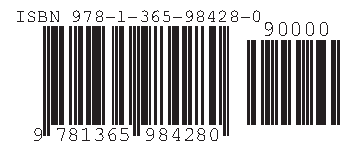
\includegraphics{isbn-barcode.pdf}

\endgroup}

\newpage

\pagestyle{empty}

~

\newpage

\addtocontents{toc}{\protect\thispagestyle{empty}}
\tableofcontents

\newpage

\pagestyle{empty}

~

\newpage

\pagestyle{plain}
\pagenumbering{arabic}

\chapter{Introduction}\label{introduction}

\begin{quote}
\textbf{In Brief}

This book shows readers how to build and deliver high-quality learning
experiences to people who want to learn how to program (and other things
as well). It is based on \href{http://software-carpentry.org}{Software
Carpentry}'s
\href{https://swcarpentry.github.io/instructor-training/}{instructor
training course}, and all material can be freely distributed and re-used
under the \href{/license/}{Creative Commons - Attribution} license.
Please see \url{http://github.com/gvwilson/teaching/} for the source,
\url{http://third-bit.com/teaching/} for the online version, and
\url{http://third-bit.com/teaching.epub} and
\url{http://third-bit.com/teaching.mobi} for e-book versions.
\end{quote}

Thousands of grassroots ``learn to code'' groups have sprung up in the
past few years. They exist so that people don't have to figure out how
to program on their own, but ironically, that's exactly what most of
their founders are doing when it comes to teaching.

As many have discovered, there's more to teaching than talking. Good
teachers break subjects up into digestible pieces, design lessons with
verifiable goals in mind, check their students' progress at short
intervals, and encourage collaboration and improvisation. Like good
programming practices, these don't have to be reinvented by every
teacher: they can and should be taught and learned. And while these
practices won't magically make someone a \emph{great} teacher, they do
make most people \emph{better} teachers.

This book is a brief introduction to modern evidence-based teaching
practices and how to use them to teach programming to free-range
learners. It covers:

\begin{itemize}
\item
  how people's thinking changes as they go from being novices to
  competent practitioners and then to being experts;
\item
  how to tell if your learners are keeping up with you, and what to do
  or say when they're not;
\item
  how to design and improve lessons efficiently and collaboratively;
\item
  how and why \href{live.html}{live coding} (i.e., writing programs step
  by step in front of learners) is a better way to teach programming
  than lectures or self-directed practice; and
\item
  how insights and techniques borrowed from the performing arts can make
  you a better teacher.
\end{itemize}

\section{History}\label{history}

I started teaching people how to program in the late 1980s. At first, I
went too fast, used too much jargon, and had little idea of how much my
learners actually understood. I got better over time, but still had no
idea how effective I was compared to other teachers.

In 2010, I rebooted a project called
\href{http://software-carpentry.org}{Software Carpentry}, whose aim is
to teach basic computing skills to researchers. In the years that
followed, I discovered resources like Mark Guzdial's blog
{[}\href{biblio.html\#guzdial-blog}{Guzdial2017}{]} and the book
\emph{How Learning Works}
{[}\href{biblio.html\#ambrose-hlw}{Ambrose2010}{]}. These led me to
{[}\href{biblio.html\#lemov-champion}{Lemov2014}{]},
{[}\href{biblio.html\#huston-dont-know}{Huston2009}{]},
{[}\href{biblio.html\#green-babt}{Green2014}{]}, and other sources that
showed me how to make my teaching better and why I should believe it
would work.

We started using these ideas in
\href{http://software-carpentry.org}{Software Carpentry} in 2012, and
the results were everything we'd hoped for. We also started offering a
short course to introduce people to these techniques and the ideas
behind them. This course was originally delivered online over multiple
weeks, but by 2014 we were teaching it in two intensive days (just like
our regular software skills workshops). Since then, I have run the
course more than forty times for people who want to teach programming to
children, recent immigrants, women re-entering the workforce, and a wide
variety of other groups. Those experiences are the basis of this book.

\section{Who You Are}\label{who-you-are}

\href{lessons.html\#learner-personas}{Learner Personas} will explain how
to define who a class is for. Here, we present personas of two typical
participants in a workshop based on this book.

\textbf{Samira} is an undergraduate student in mechanical engineering
who first encountered the subject in an after-school club for girls and
would now like to pass on her love for it. She has done one programming
class and one robotics class, and was a lab assistant for a couple of
weekend introductions to engineering for high school students at her
university. Feels insecure about standing up and teaching a subject that
she isn't an expert in (``I'm not a professor!'').

Samira would like to learn techniques for explaining ideas and handling
unexpected questions or situations. This workshop will introduce her to
some basic classroom practices and give her a chance to try them out in
front of a supportive audience.

\textbf{Moshe} is a professional programmer with two young children.
Their school doesn't offer a programming class, so he has volunteered to
put one together. He has been programming in Visual Basic and C\# for
almost twenty years, during which time he has frequently given
presentations to colleagues and management, but after reading a dozen
different ``programming for kids'' books, he feels more confused than
ever about what to do.

Moshe wants to learn how to build lessons that both he and other people
can use and maintain. This class will show him how to design and deliver
lessons tailored for his students, how to tell how well those lessons
are working, and how to keep those lessons up to date.

Moshe is partially deaf, and most of his students have hearing
disabilities as well.

\section{Teaching Practices}\label{teaching-practices}

We suggest that instructor training workshops use these three teaching
practices right from the start:

\begin{itemize}
\item
  Have a \href{practices.html\#code-of-conduct}{code of conduct}.
\item
  \href{practices.html\#take-notes-together}{Take notes together}.
\item
  \href{practices.html\#assess-motivation-and-prior-knowledge}{Pre-assess}
  learners' motivation and prior knowledge.
\end{itemize}

\section{Acknowledgments}\label{acknowledgments}

This book is the product of many contributors, including Erin Becker,
Neil Brown, Francis Castro, Warren Code, Karen Cranston, Katie
Cunningham, Neal Davis, Mark Degani, Brian Dillingham, Bob Freeman, Mark
Guzdial, Rayna Harris, Ian Hawke, Kate Hertweck, Toby Hodges, Christina
Koch, Colleen Lewis, Sue McClatchy, Lex Nederbragt, Jeramia Ory,
Elizabeth Patitsas, Aleksandra Pawlik, Emily Porta, Alex Pounds,
Danielle Quinn, Erin Robinson, Ariel Rokem, Pat Schloss, Malvika Sharan,
Tracy Teal, Richard Tomsett, Matt Turk, Fiona Tweedie, Allegra Via,
Anelda van der Walt, Stéfan van der Walt, Belinda Weaver, Hadley
Wickham, Jason Williams, and Andromeda Yelton. I am grateful to them,
and to everyone who has gone through classes based on this material over
the years.

This book is dedicated to my mother, Doris Wilson, who taught hundreds
of children to read and to believe in themselves.

\section{Challenges}\label{challenges}

\subsection{Favorite Class (10
minutes)}\label{favorite-class-10-minutes}

In the online notes, write down your name, the best class you ever took,
and what made it so great.

\chapter{Helping Novices Build Mental
Models}\label{helping-novices-build-mental-models}

\begin{quote}
\textbf{Objectives}

\begin{itemize}
\tightlist
\item
  Learners can explain the cognitive differences between novices and
  competent practitioners in terms of mental models, and explain the
  implications of these differences for teaching.
\item
  Learners can define and differentiate formative and summative
  assessment.
\item
  Learners can construct multiple-choice questions with plausible
  distractors that have diagnostic power.
\end{itemize}
\end{quote}

The first task in teaching is to figure out who your learners are and
how best to help them. Our approach is based on the
\href{https://en.wikipedia.org/wiki/Dreyfus_model_of_skill_acquisition}{Dreyfus
model of skill acquisition}, and more specifically on the work of
researchers like Patricia Benner, who studied how nurses progress from
being novices to being experts
{[}\href{biblio.html\#benner-expertise}{Benner2000}{]}. Benner
identified five stages of cognitive development that most people go
through in a fairly consistent way. (We say ``most'' and ``fairly''
because human beings are variable, and there will always be outliers.
However, that shouldn't prevent us from making strong statements about
what's true for the majority.)

For our purposes, we simplify the five stages to three:

\begin{enumerate}
\def\labelenumi{\arabic{enumi}.}
\item
  A \emph{\href{gloss.html\#novice}{novice}} is someone who doesn't know
  what they don't know, i.e., they don't yet know what the key ideas in
  the domain are or how they relate. They reason by analogy and
  guesswork, borrowing bits and pieces of their mental models of other
  domains which seem superficially similar.
\item
  A \emph{\href{gloss.html\#competent-practitioner}{competent
  practitioner}} is someone who has a mental model that's good enough
  for everyday purposes: they can do normal tasks with normal effort
  under normal circumstances. This model does not have to be completely
  accurate in order to be useful: for example, the average driver's
  mental model of how a car works probably doesn't include most of the
  complexities that a mechanical engineer would be concerned with.
\item
  An \emph{\href{gloss.html\#expert}{expert}} is someone who can easily
  handle situations that are out of the ordinary, diagnose the causes of
  problems, and so on. We will discuss expertise in more detail in
  \href{memory.html}{Memory}.
\end{enumerate}

One sign that someone is a novice is that the things they say aren't
even wrong, e.g., they think there's a difference between programs they
type in character by character and identical ones that they have copied
and pasted. As we will discuss \href{motivation.html}{later}, it is very
important not to shame novices for this.

One example of a mental model is the ball-and-spring model of molecules
that most of us encountered in high school chemistry. Atoms aren't
actually balls, and their bonds aren't actually springs, but the model
does a good job of helping people reason about chemical compounds and
their reactions. Another model of an atom has a small central ball (the
nucleus) surrounded by orbiting electrons. Again, this model is wrong,
but useful for many purposes.

Novices, competent practitioners, and experts need to be taught
differently. In particular, presenting novices with a pile of facts
early on is counter-productive, because they don't yet have a model to
fit those facts into. In fact, presenting too many facts too soon can
actually reinforce the incorrect mental model they've cobbled together.
As Derek Muller wrote about this
{[}\href{biblio.html\#muller-videos}{Muller2011}{]} in the context of
video instruction for science students:

\begin{quote}
Students have existing ideas about scientific phenomena before viewing a
video. If the video presents scientific concepts in a clear, well
illustrated way, students believe they are learning but they do not
engage with the media on a deep enough level to realize that what was is
presented differs from their prior knowledge.

There is hope, however. Presenting students' common misconceptions in a
video alongside the scientific concepts has been shown to increase
learning by increasing the amount of mental effort students expend while
watching it.
\end{quote}

The goal with novices is therefore \emph{to help them construct a
working mental model} so that they have somewhere to put facts. As an
example of what this means in practice, Software Carpentry's
\href{http://swcarpentry.github.io/shell-novice/}{lesson on the Unix
shell} introduces fifteen commands in three hours. Twelve minutes per
command may seem glacially slow, but the lesson's real purpose isn't to
teach those fifteen commands: it's to teach learners about paths,
history, tab completion, wildcards, pipes and filters, command-line
arguments, redirection, and all the other big ideas that the shell
depends on. Once they understand those concepts, people can quickly
learn a repertoire of commands. What's more, later lessons on how to
build functions in a programming language can refer back to pipes and
filters, which helps solidify both ideas.

\begin{quote}
\textbf{Different Kinds of Lessons}

The cognitive differences between novices and competent practitioners
underpin the differences between two kinds of teaching materials. A
tutorial's purpose is to help newcomers to a field build a mental model;
a manual's role, on the other hand, is to help competent practitioners
fill in the gaps in their knowledge. Tutorials frustrate competent
practitioners because they move too slowly and say things that are
obvious (though of course they are anything but to newcomers). Equally,
manuals frustrate novices because they use jargon and \emph{don't}
explain things. One of the reasons Unix and C became popular is that
Kernighan et al's trilogy
{[}\href{biblio.html\#kernighan-plauger-elements}{Kernighan1982}{]},
{[}\href{biblio.html\#kernighan-pike-upe}{Kernighan1984}{]},
{[}\href{biblio.html\#kernighan-ritchie-c}{Kernighan1988}{]} somehow
managed to be good tutorials \emph{and} good manuals at the same time.
Ray and Ray's book on Unix
{[}\href{biblio.html\#ray-ray-unix}{Ray2014}{]} and Fehily's
introduction to SQL {[}\href{biblio.html\#fehily-sql}{Fehily2008}{]} are
among the very few other books in computing that have accomplished this.
\end{quote}

One of the challenges in building a mental model is to clear away things
that \emph{don't} belong. As Mark Twain said, ``It ain't what you don't
know that gets you into trouble. It's what you know for sure that just
ain't so.''

Broadly speaking, learners' misconceptions fall into three categories:

\begin{enumerate}
\def\labelenumi{\arabic{enumi}.}
\item
  Simple \emph{factual errors}, such as believing that Vancouver is the
  capital of British Columbia (it's Victoria). These are simple to
  correct, but getting the facts right is not enough on its own.
\item
  \emph{Broken models}, such as believing that motion and acceleration
  must be in the same direction. We can address these by having them
  reason through examples to see contradictions.
\item
  \emph{Fundamental beliefs}, such as ``the world is only a few thousand
  years old'' or ``some kinds of people are just naturally better at
  programming than others''
  {[}\href{biblio.html\#patitsas-cs-grades}{Patitsas2016}{]}. These are
  often deeply connected to the learner's social identity, and so are
  resistant to evidence and cannot be reasoned away in class.
\end{enumerate}

\section{Formative Assessment}\label{formative-assessment}

Teaching is most effective when instructors have a way to identify and
clear up learners' misconceptions \emph{while they are teaching}. The
technical term for this is
\emph{\href{gloss.html\#formative-assessment}{formative assessment}},
which is assessment that takes place during the lesson in order to form
or shape it. Learners don't pass or fail formative assessments; instead,
its main purpose is to tell both the instructor and the learner how the
learner is doing, and what to focus on next. For example, a music
teacher might ask a student to play a scale very slowly in order to see
whether she is breathing correctly, and if she is not, what she should
change.

The counterpoint to formative assessment is
\emph{\href{gloss.html\#summative-assessment}{summative assessment}},
which is used at the end of the lesson to tell whether the desired
learning took place and whether the learner is ready to move on. One
example is a driving exam, which reassures the rest of society that
someone can safely be allowed on the road.

\begin{quote}
*When the cook tastes the soup, that's formative. when the guests taste
the soup, that's summative.\\
- Michael Scriven, as quoted by Debra Dirksen.
\end{quote}

\begin{quote}
\textbf{Connecting Formative and Summative Assessment}

One rule to use when designing lessons is that formative assessments
should prepare people for summative assessments: no one should ever
encounter a question on an exam for which the teaching did not prepare
them. This doesn't mean that novel problems should not appear, but that
if they do, learners should have had practice with and feedback on
tackling novel problems beforehand.
\end{quote}

In order to be useful during teaching, a formative assessment has to be
quick to administer and give an unambiguous result. The most widely used
kind of formative assessment is probably the multiple choice question
(MCQ). When designed well, these can do much more than just tell whether
someone knows something or not. For example, suppose we are teaching
children multi-digit addition. A well-designed MCQ would be:

\begin{quote}
Q: what is 37 + 15 ?

\begin{enumerate}
\def\labelenumi{\arabic{enumi}.}
\tightlist
\item
  52
\item
  42
\item
  412
\item
  43
\end{enumerate}
\end{quote}

The correct answer is 52, but each of the other answers provides
valuable insight:

\begin{itemize}
\item
  If the child answers 42, she is throwing away the carry completely.
\item
  If she answers 412, she knows that she can't just discard the carried
  1, but doesn't understand that it's actually a ten and needs to be
  added into the next column. In other words, she is treating each
  column of numbers as unconnected to its neighbors.
\item
  If she answers 43 then she knows she has to carry the 1, but is
  carrying it back into the same column it came from.
\end{itemize}

Each of these incorrect answers is a
\emph{\href{gloss.html\#plausible-distractor}{plausible distractor}}
with \emph{\href{gloss.html\#diagnostic-power}{diagnostic power}}.
``Plausible'' means that it looks like it could be right, while
``diagnostic power'' means that each of the distractors helps the
instructor figure out what to explain to that particular learner next.

A good MCQ tests for conceptual misunderstanding rather than simple
factual knowledge. If you are having a hard time coming up with
diagnostic distractors, then either you need to think more about your
learners' mental models, or your question simply isn't a good starting
point for an MCQ.

When you are trying to come up with distractors, think about questions
that learners asked or problems they had the last time you taught this
subject. If you haven't taught it before, think about your own
misconceptions or ask colleagues about their experiences. You can also
ask open-ended questions in one class to collect misconceptions about
material to be covered in a later class.

\begin{quote}
\textbf{Humor}

Instructors will often put supposedly-silly answers like ``a fish!'' on
MCQs, particularly ones intended for younger learners. However, they
don't provide any insight into learners' misconceptions, and most
learners don't actually find them funny.
\end{quote}

Instructors should use MCQs or some other kind of formative assessment
every 10-15 minutes in order to make sure that the class is actually
learning. That way, if a significant number of people have fallen
behind, only a short portion of the lesson will have to be repeated.
Additionally, most learners can only focus intensely for roughly this
long, so using formative assessments this frequently also helps them
re-focus.

Formative assessments can also be used preemptively: if you start a
class with an MCQ and everyone can answer it correctly, then you can
safely skip the part of the lecture in which you were going to explain
something that your learners already know. Doing this also helps show
learners that the instructor cares about how much they are learning, and
respects their time enough not to waste it.

But what should you do if most of the class votes for one of the wrong
answers? What if the votes are evenly spread between options? The answer
is, ``It depends.'' If the majority of the class votes for a single
wrong answer, you should go back and work on correcting that particular
misconception. If answers are pretty evenly split between options,
learners are probably guessing randomly and it's a good idea to go back
to a point where everyone was on the same page.

If most of the class votes for the right answer, but a few vote for
wrong ones, you have to decide whether you should spend time getting the
minority caught up, or whether it's more important to keep the majority
engaged. This is just one example of one of the most important rules of
teaching: no matter how hard you work, or what teaching practices you
use, you won't always be able to give everyone the help they need.

\begin{quote}
\textbf{Concept Inventories}

Given enough data, MCQs can be made surprisingly precise. The best-known
example is the
\href{https://en.wikipedia.org/wiki/Force_Concept_Inventory}{Force
Concept Inventory}, which gauges understanding of basic Newtonian
mechanics. By interviewing a large number of respondents, correlating
their misconceptions with patterns of right and wrong answers to
questions, and then improving the questions, its creators constructed a
diagnostic tool to pinpoint specific misconceptions. However, it's very
costly to do this, and students' ability to search for answers on the
internet is an ever-increasing threat to the validity of tools like
this.
\end{quote}

Designing an MCQ with plausible distractors is useful even if it is
never used in class because it forces the instructor to think about the
learners' mental models and how they might be broken--in short, to put
themselves into the learners' heads and see the topic from their point
of view.

\section{Teaching Practices}\label{teaching-practices-1}

If you haven't done so already, you should start using these three
teaching practices in your instructor training workshop:

\begin{itemize}
\item
  \href{practices.html\#sticky-notes-as-status-flags}{Use sticky notes
  as status flags} so that you can quickly see who needs help, who has
  questions, and who's ready to move on.
\item
  \href{practices.html\#sticky-notes-to-distribute-attention}{Use sticky
  notes to distribute attention} so that everyone gets a fair share of
  the instructor's time.
\item
  \href{practices.html\#minute-cards}{Use sticky notes as minute cards}
  to encourage learners to reflect on what they've just learned and to
  give instructors actionable feedback while they are still in a
  position to act on it.
\end{itemize}

\section{Challenges}\label{challenges-1}

\subsection{Your Mental Models (5
minutes)}\label{your-mental-models-5-minutes}

What is one mental model you use to frame and understand your work?
Write a few sentences describing it in the shared notes, and give
feedback on other learners' contributions.

\subsection{Symptoms of Being a Novice (5
minutes)}\label{symptoms-of-being-a-novice-5-minutes}

What are the symptoms of being a novice? I.e., what does someone do or
say that leads you to classify them as a novice in some domain?

\subsection{Modelling Novice Mental Models (20
minutes)}\label{modelling-novice-mental-models-20-minutes}

Create a multiple choice question related to a topic you intend to teach
and explain the diagnostic power of each its distractors (i.e., what
misconception each distractor is meant to identify).

When you are done, give your MCQ to a partner, and have a look at
theirs. Is the question ambiguous? Are the misconceptions plausible? Do
the distractors actually test for them? Are any likely misconceptions
\emph{not} tested for?

\subsection{Other Kinds of Formative Assessment (20
minutes)}\label{other-kinds-of-formative-assessment-20-minutes}

A good formative assessment requires people to think through a problem.
For example, consider this question from
{[}\href{biblio.html\#epstein-thinking-physics}{Epstein2002}{]}. Imagine
that you have placed a cake of ice in a bathtub and then filled the tub
to the rim with water. When the ice melts, does the water level go up
(so that the tub overflows), go down, or stay the same?

The correct answer is that the level stays the same: the ice displaces
its own weight in water, so it exactly fills the ``hole'' it has made
when it melts. Figuring this out why helps people build a model of the
relationship between weight, volume, and density.

Describe another kind of formative assessment you have seen or used and
explain how it helps both the instructor and the learner figure out
where they are and what they need to do next.

\subsection{A Different Progression (15
minutes)}\label{a-different-progression-15-minutes}

Another progression often used to describe the path from novice to
expert is the
\href{https://en.wikipedia.org/wiki/Four_stages_of_competence}{four
stages of competence}:

\begin{itemize}
\tightlist
\item
  Unconscious incompetence: the person doesn't know what they don't
  know.
\item
  Conscious incompetence: the person realizes that they don't know
  something.
\item
  Conscious competence: the person has learned how to do something, but
  can only do it while concentrating, and may still need to break things
  down into steps.
\item
  Unconscious competence: the skill has become second nature, and the
  person can do it reflexively.
\end{itemize}

Describe one or more subjects related to programming for which you are
at each of these levels.

\chapter{Teaching as a Performance
Art}\label{teaching-as-a-performance-art}

\begin{quote}
\textbf{Objectives}

\begin{itemize}
\tightlist
\item
  Learners can define \emph{jugyokenkyu} and lateral knowledge transfer
  and explain their relationship to each other.
\item
  Learners can describe and enact at least three techniques for giving
  and receiving feedback on teaching performance.
\item
  Learners can explain at least two ways in which using a rubric makes
  feedback more effective.
\end{itemize}
\end{quote}

Many people assume that teachers are born, not made. From politicians to
researchers and teachers themselves, reformers have designed systems to
find and promote those who can teach and eliminate those who can't. But
as Elizabeth Green explains
{[}\href{biblio.html\#green-babt}{Green2014}{]}, that assumption is
wrong, which is why educational reforms based on it have repeatedly
failed.

The book is written as a history of the people who have put that puzzle
together in the US. Its core begins with a discussion of what James
Stigler discovered during a visit to Japan in the early 1990s:

\begin{quote}
Some American teachers called their pattern ``I, We, You'': After
checking homework, teachers announced the day's topic, demonstrating a
new procedure (I)\ldots{} Then they led the class in trying out a sample
problem together (We)\ldots{} Finally, they let students work through
similar problems on their own, usually by silently making their way
through a worksheet (You)\ldots{}

The Japanese teachers, meanwhile, turned ``I, We, You'' inside out. You
might call their version ``You, Y'all, We.'' They began not with an
introduction, but a single problem that students spent ten or twenty
minutes working through alone (You)\ldots{} While the students worked,
the teacher wove through the students' desks, studying what they came up
with and taking notes to remember who had which idea. Sometimes the
teacher then deployed the students to discuss the problem in small
groups (Y'all). Next, the teacher brought them back to the whole group,
asking students to present their different ideas for how to solve the
problem on the chalkboard\ldots{} Finally, the teacher led a discussion,
guiding students to a shared conclusion (We).
\end{quote}

It's tempting but wrong to think that this particular teaching technique
is some kind of secret sauce. The actual key is a practice called
\emph{\href{gloss.html\#jugyokenkyu}{jugyokenkyu}}, which means ``lesson
study'':

\begin{quote}
\emph{Jugyokenkyu} is a bucket of practices that Japanese teachers use
to hone their craft, from observing each other at work to discussing the
lesson afterward to studying curriculum materials with colleagues. The
practice is so pervasive in Japanese schools that it
is\ldots{}effectively invisible.

In order to graduate, {[}Japanese{]} education majors not only had to
watch their assigned master teacher work, they had to effectively
replace him, installing themselves in his classroom first as observers
and then, by the third week, as a wobbly\ldots{}approximation of the
teacher himself. It worked like a kind of teaching relay. Each trainee
took a subject, planning five days' worth of lessons\ldots{} {[}and
then{]} each took a day. To pass the baton, you had to teach a day's
lesson in every single subject: the one you planned and the four you did
not\ldots{} and you had to do it right under your master teacher's nose.
Afterward, everyone--the teacher, the college students, and sometimes
even another outside observer--would sit around a formal table to talk
about what they saw.
\end{quote}

Putting work under a microscope in order to improve it is commonplace in
sports and music. A professional musician, for example, will dissect
half a dozen different recordings of ``Body and Soul'' or ``Smells Like
Teen Spirit'' before performing it. They would also expect to get
feedback from fellow musicians during practice and after performances.
Many other disciplines work this way too: the Japanese drew inspiration
from \href{https://en.wikipedia.org/wiki/W._Edwards_Deming}{Deming's
ideas on continuous improvement in manufacturing}, while the adoption of
code review over the last 15 years has done more to improve everyday
programming than any number of books or websites.

But this kind of feedback isn't part of teaching culture in the US, the
UK, Canada, or Australia. There, what happens in the classroom stays in
the classroom: teachers don't watch each other's lessons on a regular
basis, so they can't borrow each other's good ideas. The result is that
\emph{every teacher has to invent teaching on their own}. They may get
lesson plans and assignments from colleagues, the school board, a
textbook publisher, or the Internet, but each teacher has to figure out
on their own how to combine that with the theory they've learned in
education school to deliver an actual lesson in an actual classroom for
actual students.

Demonstration lessons, in which one teacher is in front of a room full
of students while other teachers observe, seem like a way to solve this.
However, Fincher and her colleagues studied how teaching practices are
actually transferred using both a detailed case study
{[}\href{biblio.html\#fincher-warrens-questions}{Fincher2007}{]} and
analysis of change stories
{[}\href{biblio.html\#fincher-stories-change}{Fincher2012}{]}. The
abstract of the latter paper sums up their findings:

\begin{quote}
Innovative tools and teaching practices often fail to be adopted by
educators in the field, despite evidence of their effectiveness. Naïve
models of educational change assume this lack of adoption arises from
failure to properly disseminate promising work, but evidence suggests
that dissemination via publication is simply not effective\ldots{} We
asked educators to describe changes they had made to their teaching
practice\ldots{} Of the 99 change stories analyzed, only three
demonstrate an active search for new practices or materials on the part
of teachers, and published materials were consulted in just
eight\ldots{} Most of the changes occurred locally, without input from
outside sources, or involved only personal interaction with other
educators.
\end{quote}

\noindent
Barker et al found something similar
{[}\href{biblio.html\#barker-practice-adoption}{Barker2015}{]}:

\begin{quote}
Adoption is not a ``rational action,'' however, but an iterative series
of decisions made in a social context, relying on normative traditions,
social cueing, and emotional or intuitive processes\ldots{} Faculty are
not likely to use educational research findings as the basis for
adoption decisions\ldots{} Positive student feedback is taken as strong
evidence by faculty that they should continue a practice.
\end{quote}

This phenomenon is sometimes called
\emph{\href{gloss.html\#lateral-knowledge-transfer}{lateral knowledge
transfer}}: someone sets out to teach X, but while watching them, their
audience actually learns Y as well (or instead). For example, an
instructor might set out to show people how to do a particular
statistical analysis in R, but what her learners might take away is some
new keyboard shortcuts in RStudio. Live coding makes this much more
likely because it allows learners to see the ``how'' as well as the
``what'', and \emph{jugyokenkyu} works because it creates more
opportunities for this to happen.

\section{Feedback}\label{feedback}

As the cartoon below suggests, sometimes it can be hard to receive
feedback, especially negative feedback. The process is easier and more
productive when the people involved share ground rules and expectations.
This is especially important when they have different backgrounds or
cultural expectations about what's appropriate to say and what isn't.

\begin{figure}
\centering
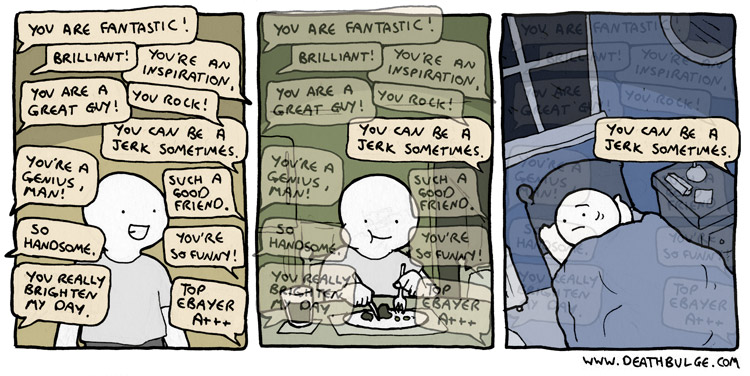
\includegraphics{fig/deathbulge-jerk.jpg}
\caption{Feedback Feelings (copyright (c) Deathbulge 2013)}
\end{figure}

You can get better feedback on your work from other people using
techniques like these:

\begin{enumerate}
\def\labelenumi{\arabic{enumi}.}
\item
  \emph{Initiate feedback.} It's better to ask for feedback than to
  receive it unwillingly.
\item
  \emph{Choose your own questions}, i.e., ask for specific feedback.
  It's a lot harder for someone to answer, ``What do you think?'' than
  to answer either, ``What is one thing I could have done as an
  instructor to make this lesson more effective?'' or ``If you could
  pick one thing from the lesson to go over again, what would it be?''

  Directing feedback like this is also more helpful to you. It's always
  better to try to fix one thing at once than to change everything and
  hope it's for the better. Directing feedback at something you have
  chosen to work on helps you stay focused, which in turn increases the
  odds that you'll see progress.
\item
  \emph{Use a feedback translator.} Have a fellow instructor (or other
  trusted person in the room) read over all the feedback and give an
  executive summary. It can be easier to hear ``It sounds like most
  people are following, so you could speed up'' than to read several
  notes all saying, ``this is too slow'' or ``this is boring''.
\item
  Most importantly, \emph{be kind to yourself}. Many of us are very
  critical of ourselves, so it's always helpful to jot down what we
  thought of ourselves \emph{before} getting feedback from others. That
  allows us to compare what we think of our performance with what others
  think, which in turn allows us to scale the former more accurately.
  For example, it's very common for people to think that they're saying
  ``um'' and ``err'' all the time, when their audience doesn't notice
  it. Getting that feedback once allows instructors to adjust their
  assessment of themselves the next time they feel that way.
\end{enumerate}

\newpage

You can give feedback to others more effectively as well:

\begin{enumerate}
\def\labelenumi{\arabic{enumi}.}
\item
  \emph{Balance positive and negative feedback.} One method is a
  ``compliment sandwich'' made up of one positive, one negative, and a
  second positive observation.
\item
  \emph{Organize your feedback using a rubric.} Most people are more
  comfortable giving and receiving feedback when they feel that they
  understand the social rules governing what they are allowed to say and
  how they are allowed to say it. A facilitator can then transcribe
  items into a shared document (or onto a whiteboard) during discussion.
\end{enumerate}

\begin{quote}
\textbf{Two by Two}

The rubric we find most useful for feedback on teaching is a 2x2 grid
whose vertical axis is labelled ``positive'' and ``negative'', and whose
horizontal axis is labelled ``content'' (what was said) and
``presentation'' (how it was said). Observers write each of their
comments in one of the grid's four squares as they are watching the
demonstration.
\end{quote}

Whatever methods are used, the most important thing to remember is
feedback on teaching is meant to be formative: its goal is to help
people figure out what they are doing well and what they still need to
work on.

\begin{quote}
\textbf{Studio Classes}

Architecture schools often include studio classes, in which students
solve small design problems and get feedback from their peers right then
and there. These classes are most effective when the instructor
critiques both the designs and the peer critiques, so that participants
are learning not only how to make buildings, but how to give and get
feedback {[}\href{biblio.html\#schon-practitioner}{Schön1984}{]}. Master
classes in music serve a similar purpose, and a few people have
experimented with using live coding at conferences or online in similar
ways.
\end{quote}

\begin{quote}
\textbf{Tells}

Everyone has nervous habits. For example, many of us become ``Mickey
Mouse'' versions of ourselves when we're nervous, i.e., we talk more
rapidly than usual, in a higher-pitched voice, and wave our arms around
more than we usually would.

Gamblers call nervous habits like this ``tells''. While these are often
not as noticeable as you would think, it's good to know whether you
pace, fiddle with your hair, look at your shoes, or rattle the change in
your pocket when you don't know the answer to a question.

You can't get rid of tells completely, and trying to do so can make you
obsess about them. A better strategy is to try to displace them, e.g.,
to train yourself to scrunch your toes inside your shoes instead of
cracking your knuckles.
\end{quote}

If you are interested in knowing more about giving and getting feedback,
you may want to read
{[}\href{biblio.html\#gormally-teaching-feedback}{Gormally2014}{]} and
discuss ways you could make peer-to-peer feedback a routine part of your
teaching. You may also enjoy
{[}\href{biblio.html\#gawande-personal-best}{Gawande2011}{]}, which
looks at the value of having a coach.

\section{How to Practice Teaching}\label{how-to-practice-teaching}

One of the key elements of instructor training is recording trainees and
having them, and their peers, critique those recordings. We were
introduced to this practice by UBC's Warren Code, who got it from the
Instructional Skills Workshop
{[}\href{biblio.html\#isw-resources}{ISW2017}{]}, and it has evolved to
the following:

\begin{enumerate}
\def\labelenumi{\arabic{enumi}.}
\item
  Split into groups of three.
\item
  Each person rotates through the roles of instructor, audience, and
  videographer. As the instructor, they have two minutes to explain one
  key idea from their research (or other work) as if they were talking
  to a class of interested high school students. The person pretending
  to be the audience is there to be attentive, while the videographer
  records the session using a cellphone or similar device.
\item
  After everyone in the group of three has finished teaching, watch the
  videos as a group. Everyone gives feedback on all three videos, i.e.,
  people give feedback on themselves as well as on others.
\item
  After everyone has given feedback on all of the videos, return to the
  main group and put all of the feedback into the notes. Again, try to
  divide positive from negative and content from presentation. Try also
  to identify each person's tells: what do they do that betrays
  nervousness, and how noticeable is it?
\end{enumerate}

It's important to record all three videos and then watch all three: if
the cycle is teach-review-teach-review, the last person to teach runs
out of time. Doing all the reviewing after all the teaching also helps
put a bit of distance between the teaching and the reviewing, which
makes the exercise slightly less excruciating.

In order for this exercise to work well:

\begin{itemize}
\item
  Let people know at the start of the class that they will be asked to
  teach something so that they have time to choose a topic. (In our
  experience, telling them this in advance of the class can be
  counter-productive, since some people will fret over how much they
  should prepare.)
\item
  Groups must be physically separated to reduce audio cross-talk between
  their recordings. In practice, this means 2-3 groups in a normal-sized
  classroom, with the rest using nearby breakout spaces, coffee lounges,
  offices, or (on one occasion) a janitor's storage closet.
\item
  People must give feedback on themselves, as well as giving feedback on
  each other, so that they can calibrate their impressions of their own
  teaching according to the impressions of other people. (We find that
  most people are harder on themselves than others are, and it's
  important for them to realize this.)
\item
  Try to make at least one mistake during the demonstration of live
  coding so that trainees can see you talk through diagnosis and
  recovery, and draw attention afterward to the fact that you did this.
\end{itemize}

The announcement of this exercise is often greeted with groans and
apprehension, since few people enjoy seeing or hearing themselves.
However, it is consistently rated as one of the most valuable parts of
the class, and also serves as an ice breaker: we want pairs of
instructors at actual workshops to give one another feedback, and that's
much easier to do once they've had some practice and have a rubric to
follow.

\begin{quote}
\textbf{Setting Up Your Teaching Environment}

If the room setup allows it, try to
\href{practices.html\#setting-up-your-own-environment}{set up your
environment} to mimic what you would use in an actual classroom: have a
glass of water handy, stand instead of sitting, and so on.
\end{quote}

\section{Challenges}\label{challenges-2}

\subsection{Give Feedback (20 minutes)}\label{give-feedback-20-minutes}

\begin{enumerate}
\def\labelenumi{\arabic{enumi}.}
\item
  Watch {[}\href{biblio.html\#wilson-bad-teaching-live}{Wilson2016}{]}
  as a group and give feedback on it. Organize feedback along two axes:
  positive vs.~negative and content vs.~presentation.
\item
  Have each person in the class add one point to a 2x2 grid on a
  whiteboard (or in the shared notes) without duplicating any points
  that are already up there.
\end{enumerate}

What did other people see that you missed? What did they think that you
strongly agree or disagree with?

\subsection{Practice Giving Feedback (45
minutes)}\label{practice-giving-feedback-45-minutes}

Use the process described above to practice teaching in groups of three.
When your group is done, the instructor will add one point of feedback
from each participant to a 2x2 grid on the whiteboard or in the shared
notes, without accepting duplicates. Participants should not say whether
the point they offer was made by them, about them, or neither: the goal
at this stage is primarily for people to become comfortable with giving
and receiving feedback, and to establish a consensus about what sorts of
things to look for.

\chapter{Expertise and Memory}\label{expertise-and-memory}

\begin{quote}
\textbf{Objectives}

\begin{itemize}
\tightlist
\item
  Learners can define expertise and explain its operation using a graph
  metaphor for cognition.
\item
  Learners can explain the difference between repetition and deliberate
  practice.
\item
  Learners can define and construct concept maps, and explain the
  benefits of externalizing cognition.
\item
  Learners can differentiate long-term and short-term memory, describe
  the capacity limits of the latter, and explain the the impact of these
  limits on teaching.
\end{itemize}
\end{quote}

The previous chapter looked at what distinguishes novices from competent
practitioners. Here, we will look at expertise: what it is, how people
acquire it, and how it can be harmful as well as helpful. We will then
see how concept maps can be used to figure out how to turn knowledge
into lessons.

To start, what do we mean when we say someone is an expert? The usual
response is that they can solve problems much faster than people who are
``merely competent'', or that they can recognize and deal with the cases
where the normal rules don't apply. They also somehow make this look
effortless: in most cases, they just know what the right answer is.

What makes someone an expert? The answer isn't just that they know more
facts: competent practitioners can memorize a lot of trivia without any
noticeable improvement to their performance. Instead, imagine for a
moment that we store knowledge as a graph in which facts are nodes and
relationships are arcs. (This is emphatically \emph{not} how our brains
work, but it's a useful metaphor.) The key difference between experts
and people who are ``merely competent'' is that experts have many more
connections, i.e., their mental models are much more densely connected.

\newpage

This metaphor helps explain many observed aspects of expert behavior:

\begin{itemize}
\item
  Experts can jump directly from a problem to its solution because there
  actually is a direct link between the two in their mind. Where a
  competent practitioner would have to reason ``A, B, C, D, E'', the
  expert can go from A to E in a single step. We call this
  \emph{intuition}, and it isn't always a good thing: when asked to
  explain their reasoning, experts often can't, because they didn't
  actually reason their way to the solution--they just recognized it.
\item
  Experts are frequently so familiar with their subject that they can no
  longer imagine what it's like to \emph{not} see the world that way. As
  a result, they are often less good at teaching the subject than people
  with less expertise who still remember what it's like to have to learn
  the things. This phenomenon is called
  \emph{\href{gloss.html\#expert-blind-spot}{expert blind spot}}, and
  while it can be overcome with training, it's part of why there is no
  correlation between how good someone is at doing research in an area
  and how good they are at teaching it
  {[}\href{biblio.html\#marsh-hattie-teaching}{Marsh2002}{]}.
\item
  Densely-connected knowledge graphs are also the basis for experts'
  \emph{\href{gloss.html\#fluid-representation}{fluid representations}},
  i.e., their ability to switch back and forth between different views
  of a problem {[}\href{biblio.html\#petre-expertise}{Petre2016}{]}. For
  example, when trying to solve a problem in mathematics, we might
  switch between tackling it geometrically and representing it as a set
  of equations to be solved.
\item
  Finally, this metaphor also explains why experts are better at
  diagnosis than competent practitioners: more linkages between facts
  makes it easier to reason backward from symptoms to causes. (And this
  in turn is why asking programmers to debug during job interviews gives
  a more accurate impression of their ability than asking them to
  program.)
\end{itemize}

\begin{quote}
\textbf{The J Word}

Experts often betray their blind spot by using the word ``just'' in
explanations, as in, ``Oh, it's easy, you just fire up a new virtual
machine and then you just install these four patches to Ubuntu and then
you just re-write your entire program in a pure functional language.''
As we discuss later in \href{motivation.html}{Motivation}, the J word
(also sometimes called the passive dismissive adjective) should be
banned from classrooms, primarily because using it gives learners the
very clear signal that the instructor thinks their problem is trivial
and that they therefore must be stupid.
\end{quote}

The graph model of knowledge explains why helping learners make
connections is as important as introducing them to facts. To use another
analogy, the more people you know in a group, the more likely you are to
remain part of that group. Similarly, the more connections a fact has to
other facts, the more likely the fact is to be remembered.

\section{Repetition vs.~Deliberate
Practice}\label{repetition-vs.deliberate-practice}

The idea that ten thousand hours of practice will make someone an expert
in some field is widely quoted, but reality is more complex. Doing
exactly the same thing over and over again is much more likely to
solidify bad habits than perfect performance. What actually works is
\emph{\href{gloss.html\#deliberate-practice}{deliberate practice}} (also
sometimes called \emph{\href{gloss.html\#reflective-practice}{reflective
practice}}), which is doing similar but subtly different things, paying
attention to what works and what doesn't, and then changing behavior in
response to that feedback to get cumulatively better.

A common progression is for people to go through three stages:

\begin{enumerate}
\def\labelenumi{\arabic{enumi}.}
\item
  They \emph{learn how to do something given feedback from others}. For
  example, they might write an essay about what they did on their summer
  holiday, and get feedback from a teacher telling them how to improve
  it.
\item
  They \emph{learn how to give feedback}. For example, they might write
  an essay about character development in \emph{The Catcher in the Rye},
  and get feedback on their critique from a teacher.
\item
  They \emph{apply what they've learned about feedback to themselves}.
  At some point, they start critiquing their own work in real time (or
  nearly so) using the critical skills they have now built up. Doing
  this is so much faster than waiting for feedback from others that
  proficiency suddenly starts to take off.
\end{enumerate}

A meta-study conducted in 2014
{[}\href{biblio.html\#macnamara-deliberate}{Macnamara2014}{]} found that
``\ldots{}deliberate practice explained 26\% of the variance in
performance for games, 21\% for music, 18\% for sports, 4\% for
education, and less than 1\% for professions.'' One explanation for this
variation is that deliberate practice works best when the rules for
evaluating success are very stable, but is less effective when there are
more factors at play (i.e., when it's harder to connect cause to
effect).

\section{Concept Maps}\label{concept-maps}

Our tool of choice to represent a knowledge graph (expert or otherwise)
is a \emph{\href{gloss.html\#concept-map}{concept map}}. A concept map
is simply a picture of someone's mental model of a domain: facts are
bubbles, and connections are labelled arcs. It is important that they
are labelled: saying ``X and Y are related'' is only helpful if we
explain what the relationship \emph{is}. And yes, one person's fact may
be another person's connection, but one of the benefits of concept
mapping is that it makes those differences explicit.

\newpage

\begin{quote}
\textbf{Externalizing Cognition}

Concept maps are just one way to represent our understanding of a
subject. For example, Andrew Abela's decision tree
{[}\href{biblio.html\#abela-chart}{Abela2009}{]} presents a mental model
of how to choose the right kind of chart for different kinds of
questions and data. Maps, flowcharts, and blueprints can also be useful
in some contexts. What each does is
\emph{\href{gloss.html\#externalized-cognition}{externalize cognition}},
i.e., make thought processes and mental models visible so that they can
be compared, contrasted, and combined.
\end{quote}

To show what concept maps look like, consider this simple `for loop in
Python:

\begin{verbatim}
for letter in "abc":
      print('*' + letter)
\end{verbatim}

whose output is:

\begin{verbatim}
*a
*b
*c
\end{verbatim}

The three key ``things'' in this loop are shown in the first part of the
figure below, but they are only half the story--and arguably, the less
important half. The second part shows the \emph{relationships} between
those things. We can go further and add two more relationships that are
usually (but not always) true as shown in the third part.

Concept maps can be used in many ways:

\begin{enumerate}
\def\labelenumi{\arabic{enumi}.}
\item
  Concept maps aid design of a lesson by helping authors figure out what
  they're trying to teach. Crucially, a concept map separates content
  from order: in our experience, people rarely wind up teaching things
  in the order in which they first drew them.
\item
  They also aid communication between lesson designers. Instructors with
  very different ideas of what they're trying to teach are likely to
  pull their learners in different directions. Drawing and sharing
  concept maps isn't guaranteed to prevent this, but it certainly helps.
\item
  Concept maps also aid communication with learners. While it's possible
  to give learners a pre-drawn map at the start of a lesson for them to
  annotate, it's better to draw it piece by piece while teaching to
  reinforce the ties between what's in the map and what the instructor
  said. (We will return to this idea when we discuss Mayer's work on
  multimedia learning in \href{load.html}{Cognitive Load}).
\item
  Concept maps are also a useful for assessment: having learners draw
  concept maps of what they think they just heard shows the instructor
  what was missed and what was mis-understood. However, reviewing
  learners' concept maps is too time-consuming for use in class, but
  very useful in weekly lectures \emph{once learners are familiar with
  the technique}. The qualification is necessary because any new way of
  doing things initially slows people down--if a student is trying to
  make sense of basic programming, asking them to figure out how to draw
  their thoughts at the same time is an unfair load. Finally, some
  instructors are skeptical of whether novices can effectively map their
  understanding, since introspection and explanation of understanding
  are generally more advanced skills than understanding itself.
\end{enumerate}

\begin{figure}
\centering
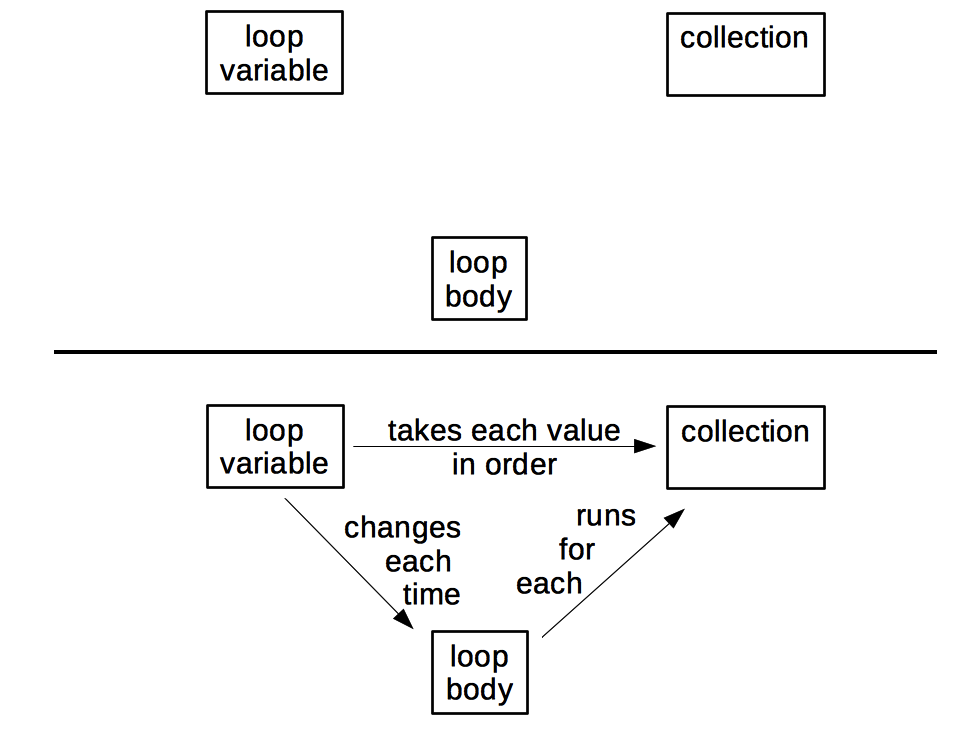
\includegraphics{fig/for-loop-concepts.png}
\caption{Concept Maps}
\end{figure}

\begin{quote}
\textbf{Meetings, Meetings, Meetings}

The next time you have a team meeting, give everyone a sheet of paper
and have them spend a few minutes drawing a concept map of the project
you're all working on--separately. On the count of three, have everyone
reveal their concept maps simultaneously. The discussion that follows
everyone's realization of how different their mental models of the
project's aims and organization are is always interesting\ldots{}
\end{quote}

\section{Seven Plus or Minus Two}\label{seven-plus-or-minus-two}

The graph model of knowledge is wrong but useful, but another simple
model has a sound physical basis. As a rough approximation, human memory
can be divided into two distinct layers. The first is called
\emph{\href{gloss.html\#long-term-memory}{long-term}} or
\emph{\href{gloss.html\#persistent-memory}{persistent memory}}. It is
where we store things like our password, our home address, and what the
clown did at our eighth birthday party that scared us so much. It is
essentially unbounded: barring injury or disease, we will die before it
fills up. However, it is also slow to access--too slow to help us handle
hungry lions and disgruntled family members.

Evolution has therefore given us a second system called
\emph{\href{gloss.html\#short-term-memory}{short-term}} or
\emph{\href{gloss.html\#working-memory}{working memory}}. It is much
faster, but also much smaller: in 1956, Miller estimated that the
average adult's working memory could hold 7±2 items for a few seconds
before things started to drop out. This is why phone numbers are
typically 7 or 8 digits long: back when phones had dials instead of
keypads, that was the longest string of numbers most adults could
remember accurately for as long as it took the dial to go around and
around. It's also why sports teams tend to have about half a dozen
members, or be broken down into smaller groups (such as the forwards and
backs in rugby).

\newpage

\begin{quote}
\textbf{Chunking}

Our minds can store larger numbers of facts in short-term memory by
creating \emph{\href{gloss.html\#chunking}{chunks}}. For example, most
of us will remember a word we read as a single item, rather than as a
sequence of letters. Similarly, the pattern made by five spots on cards
or dice is remembered as a whole rather than as five separate pieces of
information.

Chunks allow us to manage larger problems, but can also mislead us if we
mis-identify something, i.e., see it as something it isn't. We will
discuss this in more detail
\href{load.html\#pattern-recognition}{later}. Recent estimates have
suggested that the size of short-term memory might be as low as 4±1
{[}\href{biblio.html\#didau-teachers-psych}{Didau2016}{]} which means
that effective chunking (discussed below) is even more important than
first thought.
\end{quote}

7±2 is probably the most important number in programming. When someone
is trying to write the next line of a program, or understand what's
already there, she needs to keep a bunch of arbitrary facts straight in
her head: what does this variable represent, what value does it
currently hold, etc. If the number of facts grows too large, her mental
model of the program comes crashing down (something we have all
experienced).

7±2 is also the most important number in teaching. An instructor cannot
push information directly into a learner's long-term memory. Instead,
whatever she presents is first represented in the learner's short-term
memory, and is only transferred to long-term memory after it has been
held there and rehearsed. If we present too much information too
quickly, the new will displace the old before it has a chance to
consolidate in long-term memory.

This is one of the reasons to create a concept map for a lesson before
teaching it: an instructor needs to identify how many pieces of separate
information will need to be ``stored'' in memory as part of the lesson.
In practice, it's common to draw a concept map, realize that there's far
too much in it to teach in a single pass, and then carve out
tightly-connected sub-sections to divide the overall lesson into
teachable episodes.

\begin{quote}
\textbf{Building Concept Maps Together}

Concept maps can be used as a classroom discussion exercise. Put
learners in small groups (2-4 people each), give each group some sticky
notes on which a few key concepts are written, and have them build a
concept map on a whiteboard by placing those sticky notes, connecting
them with labelled arcs, and adding any other concepts they think they
need.
\end{quote}

\section{Challenges}\label{challenges-3}

\subsection{Concept Mapping (30
minutes)}\label{concept-mapping-30-minutes}

Create a hand drawn concept map for something you would teach in five
minutes. (If possible, do it for the same subject that created a
multiple choice question for earlier.) Trade with a partner, and
critique each other's maps. Do they present concepts or surface detail?
Which of the relationships in your partner's map do you consider
concepts and vice versa?

\chapter{Cognitive Load}\label{cognitive-load}

\begin{quote}
\textbf{Objectives}

\begin{itemize}
\tightlist
\item
  Learners can define cognitive load and explain how consideration of it
  can be used to shape instruction.
\item
  Learners can explain what faded examples are and construct faded
  examples for use in programming workshops.
\item
  Learners can explain what Parsons Problems are and construct Parsons
  Problems for use in programming workshops.
\item
  Learners can describe ways they differ from their own students and
  what effect those differences have on instruction.
\end{itemize}
\end{quote}

In 2006, Kirschner, Sweller, and Clark published a paper titled ``Why
Minimal Guidance During Instruction Does Not Work: An Analysis of the
Failure of Constructivist, Discovery, Problem-Based, Experiential, and
Inquiry-Based Teaching''
{[}\href{biblio.html\#kirschner-minimal}{Kirschner2006}{]}. Its abstract
says:

\begin{quote}
Although unguided or minimally guided instructional approaches are very
popular and intuitively appealing\ldots{}these approaches ignore both
the structures that constitute human cognitive architecture and evidence
from empirical studies over the past half-century that consistently
indicate that minimally guided instruction is less effective and less
efficient than instructional approaches that place a strong emphasis on
guidance of the student learning process. The advantage of guidance
begins to recede only when learners have sufficiently high prior
knowledge to provide ``internal'' guidance.
\end{quote}

The paper set off a minor academic firestorm, because beneath the jargon
the authors were claiming that
\emph{\href{gloss.html\#inquiry-based-learning}{inquiry-based learning}}
doesn't actually work very well. Inquiry-based learning is the practice
of allowing learners to ask their own questions, set their own goals,
and find their own path through a subject, just as they would when
solving problems in real life. It is intuitively appealing, but
Kirschner argued that it overloads learners, since it requires them to
simultaneously master both a domain's factual content and its
problem-solving strategies.

More specifically,
\emph{\href{gloss.html\#cognitive-load-theory}{cognitive load theory}}
posits that people have to deal with three things when they're learning:

\begin{enumerate}
\def\labelenumi{\arabic{enumi}.}
\item
  \emph{Intrinsic} load is what people have to keep in mind in order to
  carry out a learning task. In a programming class, this might be
  understanding what a variable is, or understanding how assignment in a
  programming language is different from creating a reference to a cell
  in a spreadsheet.
\item
  \emph{Germane} load is the (desirable) mental effort required to
  create linkages between new information and old, which is one of the
  things that distinguishes learning from memorization. An example might
  be learning how to loop through a collection in Python.
\item
  \emph{Extraneous} load is everything else that distracts or gets in
  the way, such as knowing that tabs look like multiple characters but
  only count as one when indenting Python code.
\end{enumerate}

According to this theory, searching for a solution strategy is an extra
burden on top of applying that strategy. We can therefore accelerate
learning by giving learners worked examples that show them a problem and
a detailed step-by-step solution, followed by a series of
\emph{\href{gloss.html\#faded-example}{faded examples}}. The first of
these presents a nearly-complete use of the same problem-solving
strategy just demonstrated, but with a small number of blanks for the
learner to fill in. The next problem is also of the same type, but has
more blanks, and so on until the learner is asked to solve the entire
problem. (The material that \emph{isn't} blank is often referred to as
\emph{\href{gloss.html\#scaffolding}{scaffolding}}, since it serves the
same purpose as the scaffolding set up temporarily at a building site.)

For example, someone teaching Python might start by explaining this:

\begin{verbatim}
# total_length(["red", "green", "blue"]) => 12
def total_length(words):
      total = 0
      for word in words:
          total += len(word)
      return total
\end{verbatim}

\noindent
then ask learners to fill in the blanks in:

\begin{verbatim}
# word_lengths(["red", "green", "blue"]) => [3, 5, 4]
def word_lengths(words):
      lengths = ____
      for word in words:
          lengths ____
      return lengths
\end{verbatim}

\newpage

\noindent
The next problem might be:

\begin{verbatim}
# join_all(["red", "green", "blue"]) => "redgreenblue"
def join_all(words):
      result = ____
      for ____ in ____:
          ____
      return result
\end{verbatim}

\noindent
and learners would finally be asked to tackle:

\begin{verbatim}
# acronymize(["red", "green", "blue"]) => "RGB"
def acronymize(words):
      ____
\end{verbatim}

Faded examples work because they introduce the problem-solving strategy
piece by piece. At each step, learners have one new problem to tackle.
As \href{practices.html\#never-a-blank-page}{discussed later}, this is
less intimidating than a blank screen or a blank sheet of paper. It also
encourages learners to think about the similarities and differences
between various approaches, which helps create the linkages in the
mental model that instructors want them to form.

The key to constructing a good faded example is to think about the
problem-solving strategy or solution pattern that it is meant to teach.
For example, the series of problems are all examples of the
\emph{accumulator pattern}, in which the results of processing items
from a collection are repeatedly added to a single variable in some way
to create the final result.

Cognitive load theory has been criticized as being
\href{https://edtechdev.wordpress.com/2009/11/16/cognitive-load-theory-failure/}{unfalsifiable}:
since there's no way to tell in advance of an experiment whether
something is germane or not, any result can be justified after the fact
by labelling things that hurt performance as ``extraneous'' and things
that don't ``germane''. However, there is no doubt that faded examples
are effective.

\begin{quote}
\textbf{Split Attention}

Research by Mayer and colleagues on the
\href{https://en.wikipedia.org/wiki/Split_attention_effect}{split-attention
effect} is closely related to cognitive load theory
{[}\href{biblio.html\#mayer-nine-ways}{Mayer2003}{]}. Linguistic and
visual input are processed by different parts of the human brain, and
linguistic and visual memories are stored separately as well. This means
that correlating linguistic, auditory, and visual streams of information
takes cognitive effort: when someone reads something while hearing it
spoken aloud, their brain can't help but check that it's getting the
same information on both channels.

Learning is therefore more effective when redundant information is
\emph{not} presented simultaneously in two different channels. For
example, people find it harder to learn from a video that has both
narration and on-screen captions than from one that has either the
narration or the captions but not both.

The key word in the previous paragraph is ``redundant''. It turns out
that it's more effective to draw a diagram piece by piece while teaching
rather than to present the whole thing at once. If parts of the diagram
appear at the same time as things are being said, the two will be
correlated in the learner's memory. Pointing at part of the diagram
later is then more likely to trigger recall of what was being said when
that part was being drawn.
\end{quote}

Another way to use cognitive load theory to construct exercises is
called a \emph{\href{gloss.html\#parsons-problem}{Parsons Problem}}. If
you are teaching someone to speak a new language, you could ask them a
question, and then give them the words they need to answer the question,
but in jumbled order. Their task is to put the words in the right order
to answer the question grammatically, which frees them from having to
think simultaneously about what to say \emph{and} how to say it.

Similarly, when teaching people to program, you can give them the lines
of code they need to solve a problem, and ask them to put them in the
right order. This allows them to concentrate on control flow and data
dependencies, i.e., on what has to happen before what, without being
distracted by variable naming or trying to remember what functions to
call. { Multiple studies have shown that Parsons Problems take less time
for learners to do, but produce equivalent educational outcomes
{[}\href{biblio.html\#ericson-parsons}{Ericons2017}{]}. }

\section{Pattern Recognition}\label{pattern-recognition}

\href{memory.html\#seven-plus-or-minus-two}{An earlier section}
described how people chunk related or correlated information together so
that they can fit more into short-term memory. One key finding in
cognition research is that experts have more and larger chunks than
non-experts, i.e., experts ``see'' larger patterns, and have more
patterns to match things against. This allows them to reason at a higher
level, and to search for information more quickly and more accurately.

It is therefore tempting to try to teach patterns directly--in fact,
supporting this is one of the reasons programmers have been so
enthusiastic about
\href{https://en.wikipedia.org/wiki/Software_design_pattern}{design
patterns}. In practice, though, pattern catalogs are too large to flick
through and too dry to memorize directly. Giving names to a small number
of patterns, though, does seem to help with teaching, primarily by
giving the learners a richer vocabulary to think and communicate with
{[}\href{biblio.html\#kuittinen-patterns}{Kuittinen2004}{]}.

\section{You Are Not Your Learners}\label{you-are-not-your-learners}

People learn best when they care about the topic and believe they can
master it. Neither fact is particularly surprising, but their practical
implications have a lot of impact on what we teach, and the order in
which we teach it.

First, as noted in \href{motivation.html}{Motivation}, most people don't
actually want to program: they want to build a website or check on
zoning regulations, and programming is just a tax they have to pay along
the way. They don't care how hash tables work, or even that hash tables
exist; they just want to know how to process data faster. We therefore
have to make sure that everything we teach is useful right away, and
conversely that we don't teach anything just because it's
``fundamental''.

Second, believing that something will be hard to learn is a
self-fulfilling prophecy. This is why it's important not to say that
something is easy: if someone who has been told that tries it, and it
doesn't work, they are more likely to become discouraged.

It's also why installing and configuring software is a much bigger
problem for us than experienced programmers like to acknowledge. It
isn't just the time we lose at the start of boot camps as we try to get
a Unix shell working on Windows, or set up a version control client on
some idiosyncratic Linux distribution.

It isn't even the unfairness of asking students to debug things that
depend on precisely the knowledge they have come to learn, but which
they don't yet have. The real problem is that every such failure
reinforces the belief that computing is hard, and that they'd have a
better chance of making next Thursday's deadline at work if they kept
doing things the way they always have. For these reasons, we have
adopted a ``teach most immediately useful first'' approach described in
\href{motivation.html}{Motivation}.

\section{Challenges}\label{challenges-4}

\subsection{Create a Faded Example (30
minutes)}\label{create-a-faded-example-30-minutes}

It's very common for programs to count how many things fall into
different categories: for example, how many times different colors
appear in an image, or how many times different words appear in a
paragraph of text.

\begin{enumerate}
\def\labelenumi{\arabic{enumi}.}
\item
  Create a short example (no more than 10 lines of code) that shows
  people how to do this, and then create a second example that solves a
  similar problem in a similar way, but has a couple of blanks for
  learners to fill in. How did you decide what to fade out? What would
  the next example in the series be?
\item
  Define the audience for your examples. For example, are these
  beginners who only know some basics programming concepts? Or are these
  learners with some experience in programming but not in Python?
\item
  Show your example to a partner, but do \emph{not} tell them what level
  it is intended for. Once they have filled in the blanks, ask them what
  level they think it is for.
\end{enumerate}

If there are people among the trainees who don't program at all, make
sure that they are in separate groups and ask to the groups to work with
that person as a learner to help identify different loads.

\subsection{Create a Parsons Problem (20
minutes)}\label{create-a-parsons-problem-20-minutes}

Write five or six lines of code that does something useful, jumble them,
and ask your partner to put them in order. If you are using an
indentation-based language like Python, do not indent any of the lines;
if you are using a curly-brace language like Java, do not include any of
the curly braces.

\chapter{Designing Lessons}\label{designing-lessons}

\begin{quote}
\textbf{Objectives}

\begin{itemize}
\tightlist
\item
  Learners can describe the steps in reverse instructional design and
  explain why it generally produces better lessons than the usual
  ``forward'' lesson development process.
\item
  Learners can define ``teaching to the test'' and explain why reverse
  instructional design is \emph{not} the same thing.
\item
  Learners can construct and critique five-part learner personas.
\item
  Learners can construct good learning objectives and critique learning
  objectives with reference to Bloom's Taxonomy and/or Fink's Taxonomy.
\end{itemize}
\end{quote}

Most people design lessons as follows:

\begin{enumerate}
\def\labelenumi{\arabic{enumi}.}
\item
  Someone tells you that you have to teach something you haven't thought
  about in ten years.
\item
  You start writing slides to explain what you know about the subject.
\item
  After two or three weeks, you make up an assignment based more or less
  on what you've taught so far.
\item
  You repeat step 3 several times.
\item
  You stay awake into the wee hours of the morning to create a final
  exam.
\end{enumerate}

There's a better way, but to explain it, we first need to explain how
\emph{\href{gloss.html\#test-driven-development}{test-driven
development}} (TDD) is used in software development. Programmers who are
using TDD don't write software and then (possibly) write tests. Instead,
they write the tests first, then write just enough new software to make
those tests pass, and then clean up a bit.

TDD works because writing tests forces programmers to specify exactly
what they're trying to accomplish and what ``done'' looks like. It's
easy to be vague when using a human language like English or Korean;
it's much harder to be vague in Python or R.

TDD also reduces the risk of endless polishing, and also the risk of
confirmation bias: someone who hasn't written a program is much more
likely to be objective when testing it than its original author, and
someone who hasn't written a program \emph{yet} is more likely to test
it objectively than someone who has just put in several hours of hard
work and really, really wants to be done.

A similar ``backward'' method works very well for lesson design. This
method is something called
\emph{\href{gloss.html\#reverse-instructional-design}{reverse
instructional design}} and was developed independent in
{[}\href{biblio.html\#wiggins-mctighe}{Wiggins2005}{]},
{[}\href{biblio.html\#biggs-tang-quality}{Biggs2011}{]}, and
{[}\href{biblio.html\#fink-significant}{Fink2013}{]} (a summary of which
is freely available online
{[}\href{biblio.html\#fink-short}{Fink2003}{]}.) In brief, lessons
should be designed as follows:

\begin{enumerate}
\def\labelenumi{\arabic{enumi}.}
\item
  Brainstorm to get a rough idea of what you want to cover, how you're
  going to do it, what problems or misconceptions you expect to
  encounter, what's \emph{not} going to be included, and so on.
\item
  Create or recycle learner personas (discussed in the next section) to
  figure out who you are trying to teach and what will appeal to them.
\item
  Draw concept maps to describe the mental model you want learners to
  construct.
\item
  Create assessments that will give the learners a chance to practice
  the things they're trying to learn and tell you and them whether
  they're making progress and where they need to focus their work.
\item
  Put the assessments in order based on their complexity and
  dependencies to construct a course outline.
\item
  Write just enough to get learners from one formative assessment to the
  next. An actual classroom lesson will typically then consist of three
  or four such episodes, each building toward a short check that
  learners are keeping up.
\end{enumerate}

This method helps to keep teaching focused on its objectives. It also
ensures that learners don't face anything on the final exam that the
course hasn't prepared them for.

\begin{quote}
\textbf{Building Lessons by Subtracting Complexity}

One way to build a programming lesson is to write the program you want
learners to finish with, then remove the most complex part that you want
them to write and make it the last exercise. You can then remove the
next most complex part you want them to write and make it the
penultimate exercise, and so on. Anything that's left--i.e., anything
you don't want them to write as an exercise--becomes the starter file(s)
that you give them. This typically includes things like importing
libraries or helper functions to access data.
\end{quote}

\begin{quote}
\textbf{How and Why to Fake It}

One of the most influential papers in the history of software
engineering was Parnas and Clements' ``A Rational Design Process: How
and Why to Fake It''. In it, the authors pointed out that in real life
we move back and forth between gathering requirements, interface design,
programming, and testing, but when we write up our work it's important
to describe it as if we did these steps one after another so that other
people can retrace our steps. The same is true of lesson design: while
we may change our mind about what we want to teach based on something
that occurs to us while we're writing an MCQ, we want the notes we leave
behind to present things in the order described above.
\end{quote}

\begin{quote}
\textbf{Teaching to the Test}

Reverse instructional design is \emph{not} the same thing as ``teaching
to the test''. When using RID, teachers set goals to aid in lesson
design, and may never actually give the final exam that they wrote. In
many school systems, on the other hand, an external authority defines
assessment criteria for all learners, regardless of their individual
situations, and the outcomes of those summative assessments directly
affect the teachers' pay and promotion. Green's \emph{Building a Better
Teacher} {[}\href{biblio.html\#green-babt}{Green2014}{]} argues that
this focus on measurement is appealing to those with the power to set
the tests, but is unlikely to improve outcomes unless it is coupled with
support for teachers to make improvements based on test outcomes. This
is often missing, because as Scott pointed out in
{[}\href{biblio.html\#scott-state}{Scott1999}{]}, large organizations
usually value uniformity over productivity.
\end{quote}

\section{Learner Personas}\label{learner-personas}

A key step in the process above is figuring out who your audience is.
One way to do this is to write two or three
\emph{\href{gloss.html\#learner-persona}{learner personas}}. This
technique is borrowed from user interface design, where short profiles
of typical users are created to help designers think about their
audience's needs, and to give them a shorthand for talking about
specific cases.

Learner personas have five parts: the person's general background, what
they already know, what \emph{they} think they want to do, how the
course will help them, and any special needs they might have. A learner
persona for a weekend workshop aimed at new college students might be:

\begin{enumerate}
\def\labelenumi{\arabic{enumi}.}
\item
  Jorge has just moved from Costa Rica to Canada to study agricultural
  engineering. He has joined the college soccer team, and is looking
  forward to learning how to play ice hockey.
\item
  Other than using Excel, Word, and the Internet, Jorge's most
  significant previous experience with computers is helping his sister
  build a WordPress site for the family business back home in Costa
  Rica.
\item
  Jorge needs to measure properties of soil from nearby farms using a
  handheld device that sends logs in a text format to his computer.
  Right now, Jorge has to open each file in Excel, crop the first and
  last points, and calculate an average.
\item
  This workshop will show Jorge how to write a little Python program to
  read the data, select the right values from each file, and calculate
  the required statistics.
\item
  Jorge can read English proficiently, but still struggles sometimes to
  keep up with spoken conversation (especially if it involves a lot of
  new jargon).
\end{enumerate}

A single learner persona is sometimes enough, but two or three that
cover the whole range of potential learners is better. One of the ways
they help is by serving as a shorthand for design issues: when speaking
with each other, lesson authors can say, ``Would Jorge understand why
we're doing this?'' or, ``What installation problems would Jorge face?''

\begin{quote}
\textbf{Our Learners Revisited}

The personas of Samira and Moshe in the \href{index.html}{introduction}
have the five points listed above, rearranged to flow more readably.
\end{quote}

\begin{quote}
\textbf{Deciding What to Teach}

There are two ways to decide what to teach: pick material and then find
an audience, or decide on an audience and then figure out what they want
to learn. Either way, Guzdial's
``\href{biblio.html\#guzdial-principles}{Five Principles for Programming
Languages for Learners}'' offers essential guidance:

\begin{enumerate}
\def\labelenumi{\arabic{enumi}.}
\tightlist
\item
  Connect to what learners know.
\item
  Keep \href{load.html}{cognitive load} low.
\item
  Be honest (i.e., use authentic tasks).
\item
  Be generative and productive.
\item
  Test your ideas rather than trusting your instincts.
\end{enumerate}
\end{quote}

\section{Learning Objectives}\label{learning-objectives}

Summative and formative assessments help instructors figure out what
they're going to teach, but in order to communicate that to learners and
other instructors, a course description should also have
\emph{\href{gloss.html\#learning-objective}{learning objectives}}
(sometimes also called a \emph{learning goal}). A learning objective is
a single sentence describing what a learner will be able to do once they
have sat through the lesson in order to demonstrate what they have
learned.

Learning objectives are meant to ensure that everyone has the same
understanding of what a lesson is supposed to accomplish. For example, a
statement like ``understand Git'' could mean any of the following, each
of this would be backed by a very different lesson:

\begin{itemize}
\item
  Learners can describe three scenarios in which version control systems
  like Git are better than file-sharing tools like Dropbox, and two in
  which they are worse.
\item
  Learners can commit a changed file to a Git repository using a desktop
  GUI tool.
\item
  Learners can explain what a detached HEAD is and recover from it using
  command-line operations.
\end{itemize}

\begin{quote}
\textbf{Objectives vs.~Outcomes}

A learning objective is what a lesson strives to achieve. A
\emph{\href{gloss.html\#learning-outcome}{learning outcome}} is what it
actually achieves, i.e., what learners actually take away. The role of
summative assessment is therefore to compare outcomes with objectives.
\end{quote}

More specifically, a good learning objective has a \emph{measurable or
verifiable verb} that states what the learner will do, and specifies the
\emph{criteria for acceptable performance}. Writing these kinds of
learning objectives may initially seem restrictive or limiting, but will
make both you, your fellow instructors, and your learners happier in the
long run. You will end up with clear guidelines for both your teaching
and assessment, and your learners will appreciate the clear
expectations.

One way to understand what makes for a good learning objective is to see
how a poor one can be improved:

\begin{itemize}
\item
  ``Learner will be given opportunities to learn good programming
  \emph{practices." Describes the lesson's content, not the attributes
  }of successful students.*
\item
  ``Learner will have a better appreciation for good programming
  \emph{practices." Doesn't start with an active verb or define the
  }level of learning, and the subject of learning has no context and
  \emph{is not specific.}
\item
  ``Learner will understand how to program in R.'' Starts with an
  \emph{active verb, but doesn't define the level of learning, and the
  }subject of learning is still too vague for assessment.*
\item
  ``Learner will write one-page read-filter-summarize-print data
  analysis scripts for tabular data using R and R Studio.'' \emph{Starts
  with an active verb, defines the level of learning, and provides
  context to ensure that outcomes can be assessed.}
\end{itemize}

\href{gloss.html\#blooms-taxonomy}{Bloom's taxonomy} can be used to
organize learning objectives. First published in 1956, it attempts to
define levels of understanding in a way that is hierarchical,
measurable, stable, and cross-cultural. The list below defines its
levels and shows some of the verbs typically used in learning objectives
written for each level.

\begin{itemize}
\item
  Knowledge: recalling learned information (name, define, recall).
\item
  Comprehension: explaining the meaning of information (restate, locate,
  explain, recognize).
\item
  Application: applying what one knows to novel, concrete situations
  (apply, demonstrate, use).
\item
  Analysis: breaking down a whole into its component parts and
  explaining how each part contributes to the whole (differentiate,
  criticize, compare).
\item
  Synthesis: assembling components to form a new and integrated whole
  (design, construct, organize).
\item
  Evaluation: using evidence to make judgments about the relative merits
  of ideas and materials (choose, rate, select).
\end{itemize}

Another way to think about learning objectives comes from
{[}\href{biblio.html\#fink-significant}{Fink2013}{]}, which defines
learning in terms of the change it is intended to produce in the
learner. \href{gloss.html\#finks-taxonomy}{Fink's Taxonomy} has six
categories:

\begin{itemize}
\tightlist
\item
  Foundational Knowledge: understanding and remembering information and
  ideas (remember, understand, identify).
\item
  Application: skills, critical thinking, managing projects (use, solve,
  calculate, create).
\item
  Integration: connecting ideas, learning experiences, and real life
  (connect, relate, compare).
\item
  Human Dimension: learning about oneself and others (come to see
  themselves as, understand others in terms of, decide to become).
\item
  Caring: developing new feelings, interests, and values (get excited
  about, be ready to, value).
\item
  Learning How to Learn: becoming a better student (identify source of
  information for, frame useful questions about).
\end{itemize}

A set of learning objectives based on this taxonomy for an introductory
course on HTML and CSS might be:

\begin{quote}
By the end of this course, students will:

\begin{itemize}
\item
  Understand the difference between markup and presentation, the nested
  nature of HTML, what CSS properties are, and how CSS selectors work.
\item
  Know how to write and style a web page using common tags and CSS
  properties.
\item
  Be able to compare and contrast authoring with HTML and CSS to
  authoring with desktop publishing tools.
\item
  Understand how the visually impaired interact and people in
  low-bandwidth environments interact with web pages and take their
  needs into account when designing new pages.
\item
  Understand the role that JavaScript plays in styling web pages and
  want to learn more about how to use it.
\item
  Be familiar with \href{https://www.w3schools.com/}{W3Schools} and
  other free tutorials for HTML and CSS, and know what search terms to
  use to find answers on \href{https://stackoverflow.com/}{Stack
  Overflow}.
\end{itemize}
\end{quote}

\section{Maintainability}\label{maintainability}

Good courses take a lot of effort to build, but building them is only
the first challenge. Once they have been written, someone needs to
maintain them, and doing that is a lot easier if the lessons have been
built in a maintainable way.

But what exactly does ``maintainable'' mean? The short answer is that a
course is maintainable if it's cheaper to update it than to replace it.
This equation depends on many factors, only some of which are under our
control:

\begin{enumerate}
\def\labelenumi{\arabic{enumi}.}
\item
  \emph{How well documented the course's design is.} If the person doing
  maintenance doesn't know (or doesn't remember) what the course is
  supposed to accomplish or why topics are introduced in a particular
  order, it will take her more time to update it. One of the reasons to
  use the template described earlier is to capture decisions about why
  each course is the way it is.
\item
  \emph{How the course's content is structured.} Version control is the
  secret sauce that allows software development to scale, but today's
  version control systems (still) can't handle widely-used file formats
  like Word and PowerPoint. Lessons should therefore either be written
  in plain-text formats like HTML, Markdown, or LaTeX, or stored online
  in systems like Google Docs that allow many people to edit the same
  files. (The next section discusses this in more detail.)
\item
  \emph{How easy it is for collaborators to collaborate technically.}
  Lesson authors usually share material by passing it from hand to hand
  (or equivalently, by emailing files to each other or putting them in a
  shared drive. Collaborative writing tools like
  \href{http://docs.google.com}{Google Docs} and wikis are a big
  improvement, as they allow many people to update the same document and
  comment on other people's updates. The version control systems used by
  programmers, such as \href{http://github.com}{GitHub}, are another big
  advance, since they let any number of people work independently and
  then merge their changes back together in a controlled, reviewable
  way. Unfortunately, version control systems have a long, steep
  learning curve, which makes shared online authoring systems like
  \href{http://docs.google.com}{Google Docs} and wikis the best
  technical choice for most groups.
\end{enumerate}

\begin{quote}
\textbf{The True Cost of Video}

Making a small change to this webpage only takes a few minutes, but in
our experience, making any kind of change to a video takes an hour or
more. In addition, most people are much less comfortable recording
themselves than contributing written material.
\end{quote}

The fourth factor, and the most important one in practice, is \emph{how
willing people are to collaborate}. The tools needed to build a
``Wikipedia for lessons'' or a ``GitHub for lessons'' have been around
for almost twenty years, but neither model has caught on. When asked why
not, teachers raise
\href{http://blog.mrmeyer.com/2016/why-secondary-teachers-dont-want-a-github-for-lesson-plans/}{many
objects}, none of which hold up to close inspection:

\begin{itemize}
\item
  \emph{The most important thing about a lesson isn't having it, but
  }writing\emph{ it, because that gives you a chance to figure out what
  you think about the topic.} This objection rhymes with my personal
  experience, but the same is true of software, and somehow we get
  up-and-coming programmers to use and improve libraries rather than
  building their own stuff from scratch.
\item
  \emph{It's just more trouble than it's worth, because it's always
  easier in the short term to write something from scratch than to learn
  your way around someone else's material.} And yet most teachers use
  textbooks, and most actors perform other people's plays, and\ldots{}
\item
  \emph{It doesn't pay off for most teachers because they only teach any
  particular lesson once a year (or once a quarter).} Infrequent
  teaching ought to push people \emph{toward} re-use, not away from it.
\item
  \emph{Working at scale results in a more neutral point of view (the
  average of the contributors' personal views), but in many fields,
  lessons are valuable precisely because they're one person's opinion.}
  This is true for literature, but for basic algebra? And if the
  difference is one of teaching method rather than content, then yeah,
  there should be half a dozen different shared lessons on polynomials,
  each approaching the topic in a different way.
\item
  \emph{There's no onboarding process to teach people the mechanics of
  distributed ad hoc large-scale collaboration.} This is undoubtedly a
  contributing factor, but (a) teachers get more training in how to
  develop lessons than most programmers get in how to take part in an
  open source project and (b) lack of a formal onboarding process hasn't
  slowed down Wikipedia.
\item
  \emph{Collaboration on lesson development gets squeezed out by more
  important things (where ``important'' means ``to the principal or
  chair'').} Again, this should push people \emph{toward} collaboration
  (possibly under official radar), since every minute they don't spend
  writing a lesson is a minute they can use to satisfy the principal or
  chair.
\item
  \emph{The Firewall of Doom at many schools prevents people from
  working on shared materials.} Probably true for some people, but this
  is not true for all and most teachers in industrialized countries have
  access to a computer at home these days.
\item
  \emph{The stakes are too high for teachers who are going to be
  evaluated on their teaching.} This may be true for some teachers, but
  isn't a universal.
\item
  \emph{No measurable outcome will show improvement, so there's no
  incentive to do it.} The same is true of open source software, but
  while only a small minority of programmers contribute, that's still
  enough people for it to thrive.
\item
  \emph{It's a generational thing: as digital natives, tomorrow's
  teachers will just naturally do it.} Millenials don't actually act
  that differently from their elders, and ``not yet'' arguments are as
  unfalsifiable as the claims by members of millenarian movements that
  the apocalypse is definitely coming--yup, any day now.
\item
  \emph{You can't run regression tests on a lesson, so there's no easy
  way to }tell if my changes have broken something that you wrote.* But
  Wikipedia\ldots{}
\end{itemize}

One interesting observation is that while teachers don't collaborate at
scale, they \emph{do} remix by finding other people's materials online
or in textbooks and reworking them. That suggests that the root problem
may be a flawed analogy: rather than lesson development being like
writing Wikipedia articles or open source software, perhaps it's more
like postmodern music.

If this is true, then lessons may be the wrong granularity for sharing,
and collaboration might be more likely to take hold if the thing being
collaborated on was smaller. This fits well with Caulfield's theory of
\href{https://hapgood.us/2016/05/13/choral-explanations/}{choral
explanations}. He argues that sites like
\href{https://stackoverflow.com/}{Stack Overflow} succeed because they
provide a chorus of answers for every question, each of which is most
suitable for a slightly different questioner. If Caulfield is right, the
future of learning--particularly online learning--may lie in guided
tours of community-curated Q\&A repositories rather than in things we
would recognize as ``lessons'' today.

\section{A Reminder}\label{a-reminder}

When designing a lesson, you must always remember that \emph{you are not
your learners}. You may be older (or younger, if you're teaching
seniors) or wealthier (and therefore able to afford to download videos
without foregoing a meal to pay for the bandwidth), but you are almost
certainly more knowledgeable about technology. Don't assume that you
know what they need or will understand: ask them, and actually pay
attention to their answer. After all, it's only fair that learning
should go both ways.

\section{Challenges}\label{challenges-5}

\subsection{Learner Personas (30
minutes)}\label{learner-personas-30-minutes}

Working in pairs or small groups, create a five-point persona that
describes one of your typical learners.

\subsection{Write Learning Objectives (20
minutes)}\label{write-learning-objectives-20-minutes}

Write one more learning objectives for something you currently teach or
plan to teach using Bloom's Taxonomy. Working with a partner, critique
and improve the objectives.

\subsection{Write More Learning Objectives (20
minutes)}\label{write-more-learning-objectives-20-minutes}

Write one more learning objectives for something you currently teach or
plan to teach using Fink's Taxonomy. Working with a partner, critique
and improve the objectives.

\chapter{Motivation and Demotivation}\label{motivation-and-demotivation}

\begin{quote}
\textbf{Objectives}

\begin{itemize}
\tightlist
\item
  Learners can name and describe the three principal ways in which they
  can demotivate their own learners.
\item
  Learners can define impostor syndrome and stereotype threat, and
  describe ways in which to combat each.
\item
  Learners can describe the difference between fixed and growth mindset
  and explain the importance of encouraging the latter.
\item
  Learners can describe and enact at least three things they can do to
  make their programming workshops more accessible.
\item
  Learners can describe and enact at least three things they can do to
  make their programming workshops more inclusive.
\end{itemize}
\end{quote}

Learners need encouragement to step out into unfamiliar terrain, so this
chapter discusses ways instructors can motivate them. More importantly,
it discusses ways that we can accidentally \emph{demotivate} them, and
how we can avoid doing that.

People learn best when they care about the topic and believe they can
master it. This presents us with a problem because most people don't
actually want to program: they want to make music or compare changes to
zoning laws with family incomes, and rightly regard programming as a tax
they have to pay in order to do so. In addition, their early experiences
with programming are often demoralizing, and believing that something
will be hard to learn is a self-fulfilling prophecy.

Imagine a grid whose axes are labelled ``mean time to master'' and
``usefulness once mastered''. Everything that's quick to master, and
immediately useful should be taught first; things in the opposite corner
that are hard to learn and have little near-term application don't
belong in this course.

\begin{quote}
\textbf{Actual Time}

Any useful estimate of how long something takes to master must take into
account how frequent failures are and how much time is lost to them. For
example, editing a text file seems like a simple task, but most
graphical editors save things to the user's desktop or home directory.
If people need to run shell commands on the files they've edited, a
substantial fraction won't be able to navigate to the right directory
without help. If this seems like a small problem to you, please revisit
the discussion of expert blind spot in \href{memory.html}{Memory}.
\end{quote}

Many of the foundational concepts of computer science, such as
computability, inhabit the ``useful but hard to learn'' corner of the
grid described above. This doesn't mean that they aren't worth learning,
but if our aim is to convince people that they \emph{can} learn this
stuff, and that doing so will help them do more science faster, they are
less compelling than things like automating repetitive tasks.

We therefore recommend a ``teach most immediately useful first''
approach. Have learners do something that \emph{they} think is useful in
their daily work within a few minutes of starting each lesson. This not
only motivates them, it also helps build their confidence in us, so that
if it takes longer to get to the payoff of a later topic, they'll stick
with us.

The best-studied use of this idea is the media computation approach
developed by Guzdial and Ericson at Georgia Tech
{[}\href{biblio.html\#guzdial-mediacomp-retrospective}{Guzdial2013}{]}.
Instead of printing ``hello world'' or summing the first ten integers,
their students' first program opens an image, resizes it to create a
thumbnail, and saves the result. This is an
\emph{\href{gloss.html\#authentic-task}{authentic task}}, i.e.,
something that learners believe they would actually do in real life. It
is also has a \emph{\href{gloss.html\#tangible-artifact}{tangible
artifact}}: if the image comes out the wrong size, learners have a
concrete starting point for debugging.

\begin{quote}
\textbf{Strategies for Motivating Learners}

{[}\href{biblio.html\#ambrose-hlw}{Ambrose2010}{]} contains a list of
evidence-based methods to motivate learners. None of them are
surprising--it's hard to imagine someone saying that we \emph{shouldn't}
identify and reward what we value--but it's useful to check lessons
against these points to make sure they're doing at least a few of these
things.

What's missing from this list is strategies to motivate the
\emph{instructor}. Learners respond to an instructor's enthusiasm, and
instructors need to care about a topic in order to keep teaching it,
particularly when they are volunteers.
\end{quote}

\section{Demotivation}\label{demotivation}

\begin{quote}
\emph{Women aren't leaving computing because they don't know what it's
like; they're leaving because they \textbf{do} know.}\\
-- variously attributed
\end{quote}

If you are teaching free-range learners, they are probably already
motivated--if they weren't, they wouldn't be in your classroom. The
challenge is therefore not to demotivate them. Unfortunately, we can do
this by accident much more easily than you might think.

The three most powerful demotivators are \emph{unpredictability},
\emph{indifference}, and \emph{unfairness}. Unpredictability demotivates
people because if there's no reliable connection between what they do
and what outcome they achieve, there's no reason for them to try to do
anything. If learners believe that the instructor or the educational
system doesn't care about them or the lesson, they won't care either.
And if people believe the class is unfair, they will also be
demotivated, even if it is unfair in their favor (because consciously or
unconsciously they will worry that they will some day find themselves in
the group on the losing end
{[}\href{biblio.html\#wilkinson-pickett-spirit-level}{Wilkinson2011}{]}).
In extreme situations, learners may develop
\href{gloss.html\#learned-helplessness}{learned helplessness}: when
repeatedly subjected to negative feedback that they have no way to
escape, they may learn not to even try to escape when they could.

Here are some quick ways to demotivate your learners:

\begin{itemize}
\item
  A ``holier-than-thou'' or contemptuous attitude from an instructor.
\item
  Tell learners they are rubbish because they use Excel and/or Word,
  don't modularize their code, etc.
\item
  Repeatedly make digs about Windows and praise Linux, e.g., say that
  the former is for amateurs.
\item
  Criticize GUI applications (and by implication their users) and
  describe command-line tools as the One True Way.
\item
  Dive into complex or detailed technical discussion with the one or two
  people in the audience who clearly don't actually need to be there.
\item
  Pretend to know more than you do. People will actually trust you more
  if you are frank about the limitations of your knowledge, and will be
  more likely to ask questions and seek help.
\item
  Use the J word (``just''). As discussed in \href{memory.html}{Memory},
  this signals to the learner that the instructor thinks their problem
  is trivial and by extension that they therefore must be stupid for not
  being able to figure it out.
\item
  Feign surprise. Saying things like ``I can't believe you don't know
  X'' or ``you've never heard of Y?'' signals to the learner that they
  do not have some required pre-knowledge of the material you are
  teaching, that they are in the wrong place, and it may prevent them
  from asking questions in the future.
\end{itemize}

\begin{quote}
\textbf{Code of Conduct Revisited}

As noted \href{index.html}{at the start}, we believe very strongly that
classes should have a \href{conduct.html}{Code of Conduct}. Its details
are important, but the most important thing about it is that it exists:
knowing that we have rules tells people a great deal about our values
and about what kind of learning experience they can expect.
\end{quote}

\begin{quote}
\textbf{Never Learn Alone}

One way to support learners who have been subject to systematic
exclusion or discrimination (overt or otherwise) is to have people sign
up for workshops in small teams rather than as individuals. If an entire
lab group comes, or if attendees are drawn from the same (or
closely-related) disciplines, everyone in the room will know in advance
that they will be with at least a few people they trust, which increases
the chances of them actually coming. It also helps after the workshop:
if people come with their friends or colleagues, they can work together
to implement what they've learned.
\end{quote}

\section{Impostor Syndrome}\label{impostor-syndrome}

\emph{\href{gloss.html\#impostor-syndrome}{Impostor syndrome}} is the
belief that one is not good enough for a job or position, that one's
achievements are lucky flukes, and an accompanying fear of being ``found
out''. Impostor syndrome seems to be particularly common among
\href{https://www.usenix.org/blog/impostor-syndrome-proof-yourself-and-your-community}{high
achievers who undertake publicly visible work}.

Academic work is frequently undertaken alone or in small groups but the
results are shared and criticized publicly. In addition, we rarely see
the struggles of others, only their finished work, which can feed the
belief that everyone else finds it easy. Women and minority groups who
already feel additional pressure to prove themselves in some settings
may be particularly affected.

Two ways of dealing with your own impostor syndrome are:

\begin{enumerate}
\def\labelenumi{\arabic{enumi}.}
\item
  Ask for feedback from someone you respect and trust. Ask them for
  their honest thoughts on your strengths and achievements, and commit
  to believing them.
\item
  Look for role models. Who do you know who presents as confident and
  capable? Think about how they conduct themselves. What lessons can you
  learn from them? What habits can you borrow? (Remember, they quite
  possibly also feel as if they are making it up as they go.)
\end{enumerate}

As an instructor, you can help people with their impostor syndrome by
sharing stories of mistakes that you have made or things you struggled
to learn. This reassures the class that it's OK to find topics hard.
Being open with the group makes it easier to build trust and make
students confident to ask questions. (Live coding is great for this:
typos let the class see you're not superhuman.)

You can also emphasize that you want questions: you are not succeeding
as a teacher if no one can follow your class, so you're asking students
for their help to help you learn and improve. Remember, it's much more
important to \emph{be} smart than to \emph{look} smart.

The Ada Initiative has some excellent resources for teaching about and
dealing with imposter syndrome
{[}\href{biblio.html\#ada-imposter}{Ada2017}{]}.

\section{Stereotype Threat}\label{stereotype-threat}

Reminding people of negative stereotypes, even in subtle ways, makes
them anxious about the risk of confirming those stereotypes, which in
turn reduces their performance. This is called
\emph{\href{gloss.html\#stereotype-threat}{stereotype threat}}, and the
clearest examples in computing are gender-related. Depending on whose
numbers you trust, only 12-18\% of programmers are women, and those
figures have actually been getting worse over the last 20 years. There
are many reasons for this (see
{[}\href{biblio.html\#margolis-fisher-clubhouse}{Margolis2003}{]} and
{[}\href{biblio.html\#margolis-shallow}{Margolis2010}{]}), and
{[}\href{biblio.html\#steele-vivaldi}{Steele2011}{]} summarizes what we
know about stereotype threat in general and presents some strategies for
mitigating it in the classroom.

However, while there's lots of evidence that unwelcoming climates
demotivate members of under-represented groups, it's not clear that
stereotype threat is the underlying mechanism. Part of the problem is
that
\href{http://www.europhd.net/html/_onda02/07/PDF/20th_lab_materials/jane/shapiro_neuberg_2007.pdf}{the
term has been used in many ways}; another is
\href{https://www.psychologytoday.com/blog/rabble-rouser/201512/is-stereotype-threat-overcooked-overstated-and-oversold}{questions
about the replicability of key studies}. What \emph{is} clear is that we
need to avoid thinking in terms of a deficit model (i.e., we need to
change the members of under-represented groups because they have some
deficit, such as lack of prior experience) and instead use a systems
approach (i.e., we need to change the system because it produces these
disparities).

A great example of how stereotypes work in general was presented in
Patitsas et al's ``Evidence That Computer Science Grades Are Not
Bimodal'' {[}\href{biblio.html\#patitsas-cs-grades}{Patitsas2016}{]}.
This thought-provoking paper showed that people see evidence for a
``geek gene'' where none exists. As the paper's abstract says:

\begin{quote}
Although it has never been rigorously demonstrated, there is a common
belief that CS grades are bimodal. We statistically analyzed 778
distributions of final course grades from a large research university,
and found only 5.8\% of the distributions passed tests of multimodality.
We then devised a psychology experiment to understand why CS educators
believe their grades to be bimodal. We showed 53 CS professors a series
of histograms displaying ambiguous distributions and asked them to
categorize the distributions. A random half of participants were primed
to think about the fact that CS grades are commonly thought to be
bimodal; these participants were more likely to label ambiguous
distributions as ``bimodal''. Participants were also more likely to
label distributions as bimodal if they believed that some students are
innately predisposed to do better at CS. These results suggest that
bimodal grades are instructional folklore in CS, caused by confirmation
bias and instructor beliefs about their students.
\end{quote}

It's easy to use language that suggests that some people are natural
programmers and others aren't, but Mark Guzdial has called this belief
\href{http://cacm.acm.org/blogs/blog-cacm/189498-top-10-myths-about-teaching-computer-science/fulltext}{the
biggest myth about teaching computer science}.

\section{Mindset}\label{mindset}

Learners can be demotivated in subtler ways as well. For example, Dweck
and others have studied the differences of
\href{gloss.html\#fixed-mindset}{fixed mindset} and
\href{gloss.html\#growth-mindset}{growth mindset}. If people believe
that competence in some area is intrinsic (i.e., that you either ``have
the gene'' for it or you don't), \emph{everyone} does worse, including
the supposedly advantaged. The reason is that if they don't get it at
first, they figure they just don't have that aptitude, which biases
future performance. On the other hand, if people believe that a skill is
learned and can be improved, they do better on average.

A person's mindset can be shaped by subtle cues. For example, if a child
is told, ``You did a good job, you must be very smart,'' they are likely
to develop a fixed mindset. If on the other hand they are told, ``You
did a good job, you must have worked very hard,'' they are likely to
develop a growth mindset, and subsequently achieve more. Studies have
also shown that the simple action of telling learners about the
different mindsets before a course can improve learning outcomes for the
whole group.

As with stereotype threat,
\href{http://www.learningspy.co.uk/psychology/growth-mindset-bollocks/}{there
are concerns} that research on grown mindset has been oversold, or will
be much more difficult to put into practice than its more enthusiastic
advocates have implied. While some people interpret this back and forth
of claim and counter-claim as evidence than education research isn't
reliable, what it really shows is that anything involving human subjects
is both subtle and difficult.

\section{Accessibility}\label{accessibility}

Not providing equal access to lessons and exercises is about as
demotivating as it gets. The older Software Carpentry lessons, for
example, the text beside the slides includes all of the narration--but
none of the Python source code. Someone using a
\href{https://en.wikipedia.org/wiki/Screen_reader}{screen reader} would
therefore be able to hear what was being said about the program, but
wouldn't know what the program actually was.

While it may not be possible to accommodate everyone's needs, it
\emph{is} possible to get a good working structure in place without any
specific knowledge of what specific disabilities people might have.
Having at least some accommodations prepared in advance also makes it
clear that hosts and instructors care enough to have thought about
problems in advance, and that any additional concerns are likely to be
addressed.

\begin{quote}
\textbf{It Helps Everyone}

\href{https://en.wikipedia.org/wiki/Curb_cut}{Curb cuts} (the small
sloped ramps joining a sidewalk to the street) were originally created
to make it easier for the physically disabled to move around, but proved
to be equally helpful to people with strollers and grocery carts.
Similarly, steps taken to make lessons more accessible to people with
various disabilities also help everyone else. Proper captioning of
images, for example, doesn't just give screen readers something to say:
it also makes the images more findable by exposing their content to
search engines.
\end{quote}

The first and most important step in making lessons accessible is to
\emph{involve people with disabilities in decision-making}: the slogan
\emph{\href{https://en.wikipedia.org/wiki/Nothing_About_Us_Without_Us}{nihil
de nobis, sine nobis}} (literally, ``nothing about us, without us'')
predates accessibility rights, but is always the right place to start. A
few other recommendations are:

\begin{itemize}
\item
  \emph{Find out what you need to do.} The W3C Accessibility
  Initiative's checklist for presentations
  {[}\href{biblio.html\#w3c-accessibility}{W3C2017}{]} is a good
  starting point focused primarily on assisting the visually impaired,
  while Liz Henry's blog post about accessibility at conferences
  {[}\href{biblio.html\#henry-accessibility}{Henry2014}{]} has a good
  checklist for people with mobility issues, and this interview with
  Chad Taylor is a good introduction to issues faced by the hearing
  impaired {[}\href{biblio.html\#taylor-interview}{Taylor2014}{]}.
\item
  \emph{Know how well you're doing.} For example, sites like
  \href{http://webaim.org/}{WebAIM} allow you to check how accessible
  your online materials are to visually impaired users.
\item
  \emph{Don't do everything at once.} We don't ask learners in our
  workshops to adopt all our best practices or tools in one go, but
  instead to work things in gradually at whatever rate they can manage.
  Similarly, try to build in accessibility habits when preparing for
  workshops by adding something new each time.
\item
  \emph{Do the easy things first.} There are plenty of ways to make
  workshops more accessible that are both easy and don't create extra
  cognitive load for anyone: font choices, general text size, checking
  in advance that your room is accessible via an elevator or ramp, etc.
\end{itemize}

\section{Inclusivity}\label{inclusivity}

\emph{\href{gloss.html\#inclusivity}{Inclusivity}} is a policy of
including people who might otherwise be excluded or marginalized. In
computing, it means making a positive effort to be more welcoming to
women, people of color, people with various sexual orientations, the
elderly, the physically challenged, the formerly incarcerated, the
economically disadvantaged, and everyone else who doesn't fit Silicon
Valley's white/Asian male demographic. Lee's paper ``What can I do today
to create a more inclusive community in CS?''
{[}\href{biblio.html\#lee-create-inclusive-community}{Lee2017}{]} is a
brief, practical guide to doing that with references to the research
literature. These help learners who belong to one or more marginalized
or excluded groups, but help motivate everyone else as well; while they
are phrased in terms of term-long courses, many can be applied in our
workshops:

\begin{itemize}
\item
  Ask learners to email you before the workshop to explain how they
  believe the training could help them achieve their goals.
\item
  Review notes to make sure they are free from gendered pronouns, that
  they include culturally diverse names, etc.
\item
  Emphasize that what matters is the rate at which they are learning,
  not the advantages or disadvantages they had when they started.
\item
  Encourage pair programming.
\item
  Actively mitigate behavior that some learners may find intimidating,
  e.g., use of jargon or ``questions'' that are actually asked to
  display knowledge.
\end{itemize}

\section{Challenges}\label{challenges-6}

\subsection{Authentic Tasks (15
minutes)}\label{authentic-tasks-15-minutes}

Think about something you did this week that uses one or more of the
skills you teach, (e.g., wrote a function, bulk downloaded data, did
some stats in R, forked a repo) and explain how you would use it (or a
simplified version of it) as an exercise or example in class.

Pair up with your neighbor and decide where this exercise fits on a 2x2
grid of ``short/long time to master'' and ``low/high usefulness''? In
the shared notes, write the task and where it fits on the grid. As a
group, discuss how these relate back to the ``teach most immediately
useful first'' approach.

\subsection{Implement One Strategy for Inclusivity (5
minutes)}\label{implement-one-strategy-for-inclusivity-5-minutes}

Pick one activity or change in practice from Lee's paper
{[}\href{biblio.html\#lee-create-inclusive-community}{Lee2017}{]} that
you would like to work on. Put a reminder in your calendar three months
in the future to self-check whether you have done something about it.

\subsection{Brainstorming Motivational Strategies (20
minutes)}\label{brainstorming-motivational-strategies-20-minutes}

\begin{enumerate}
\def\labelenumi{\arabic{enumi}.}
\item
  Think back to a programming course (or any other) that you took in the
  past, and identify one thing the instructor did that demotivated you,
  and describe what could have been done afterward to correct the
  situation.
\item
  Pair up with your neighbor and discuss your stories, then add your
  comments to the shared notes.
\item
  Review the comments in the shared notes as a group. Rather than read
  them all out loud, highlight and discuss a few of the things that
  could have been done differently. This will give everyone some
  confidence in how to handle these situations in the future.
\end{enumerate}

\subsection{Demotivational Experiences (15
minutes)}\label{demotivational-experiences-15-minutes}

Think back to a time when you demotivated a student (or when you were
demotivated as a student). Pair up with your neighbor and discuss what
you could have done differently in the situation, and then share the
story and what could have been done in the group notes.

\subsection{Walk the Route (15
minutes)}\label{walk-the-route-15-minutes}

Find the nearest public transportation drop-off point to your building
and walk from there to your office and then to the nearest washroom,
making notes about things you think would be difficult for someone with
mobility issues. Now borrow a wheelchair and repeat the journey. How
complete was your list of challenges? And did you notice that the first
sentence in this challenge assumed you could actually walk?

\subsection{Who Decides? (15 minutes)}\label{who-decides-15-minutes}

In {[}\href{biblio.html\#littky-big-picture}{Littky2004}{]}, Kenneth
Wesson wrote, ``If poor inner-city children consistently outscored
children from wealthy suburban homes on standardized tests, is anyone
naive enough to believe that we would still insist on using these tests
as indicators of success?'' Read
{[}\href{biblio.html\#cottrill-gifted}{Cottrill2016}{]}, and then
describe an example from your own experience of ``objective''
assessments that reinforced the status quo.

\subsection{Credibility}\label{credibility}

{[}\href{biblio.html\#fink-significant}{Fink2013}{]} describes three
things that make teachers credible in their learners' eyes:

\begin{itemize}
\item
  \textbf{Competence}, or knowledge of the subject, as shown by the
  ability to explain complex ideas or reference the work of others.
\item
  \textbf{Trustworthiness}, or having the student's best interests in
  mind. This can be shown by giving individualized feedback, offering a
  rational explanation for grading decisions, and treating all students
  the same.
\item
  \textbf{Dynamism}, or excitement about the subject. This was discussed
  in detail in the chapter on \href{performance.html}{teaching as a
  performance art}.
\end{itemize}

Describe one thing you do when teaching that fits into each category,
and then describe one thing you \emph{don't} do but should for each
category as well

\chapter{Live Coding}\label{live-coding}

\begin{quote}
\textbf{Objectives}

\begin{itemize}
\tightlist
\item
  Learners can describe live coding and explain its advantages as a
  teaching practice for programming workshops.
\item
  Learners can enact and critique live coding.
\end{itemize}
\end{quote}

\begin{quote}
\emph{Teaching is theater not cinema.}\\
-- Neal Davis
\end{quote}

Teaching is a performance art, just like drama, music, and athletics.
And as in those fields, we have a collection of small tips and tricks to
make teaching work better.

The first of our recommended teaching practices is so central that it
deserves a chapter of its own: \emph{\href{gloss.html\#live-coding}{live
coding}}. When they are live coding, instructors don't use slides.
Instead, they go through the lesson material, typing in the code or
instructions, with their learners following along. Its advantages are:

\begin{enumerate}
\def\labelenumi{\arabic{enumi}.}
\item
  Watching a program being written is more compelling than watching
  someone page through slides that present bits and pieces of the same
  code.
\item
  It enables instructors to be more responsive to ``what if?''
  questions. Where a slide deck is like a railway track, live coding
  allows instructors to go off road and follow their learners'
  interests.
\item
  It facilitates lateral knowledge transfer: people learn more than we
  realized we were teaching by watching \emph{how} instructors do
  things.
\item
  It slows the instructor down: if she has to type in the program as she
  goes along, she can only go twice as fast as her learners, rather than
  ten-fold faster as she could with slides.
\item
  Learners get to see instructors' mistakes \emph{and how to diagnose
  and correct them}. Novices are going to spend most of their time doing
  this, but it's left out of most textbooks.
\item
  Watching instructors make mistakes shows learners that it's all right
  to make mistakes of their own. Most people model the behavior of their
  teachers: if the instructor isn't embarrassed about making and talking
  about mistakes, learners will be more comfortable doing so too.
\end{enumerate}

Live coding does have some drawbacks, but with practice, these can be
avoided or worked around:

\begin{enumerate}
\def\labelenumi{\arabic{enumi}.}
\item
  Instructors can go too slowly, either because they are not good
  typists or by spending too much time looking at notes to try to
  remember what they meant to type.
\item
  Typing in boilerplate code that is needed by the lesson, but not
  directly relevant to it (such as library import statements) increases
  the \href{load.html}{extraneous cognitive load} on your learners.
  Willingham says ``Memory is the residue of thought''
  {[}\href{biblio.html\#willingham-dont-like-school}{Willingham2010}{]},
  so if you spend your time typing boilerplate, that may be what
  learners will take away.
\end{enumerate}

Live coding is an example of the ``I/We/You'' approach to teaching
discussed in \href{performance.html}{Performance}. It takes a bit of
practice for instructors to get used to thinking aloud while coding in
front of an audience, but most report that it is then no more difficult
to do than talking off a deck of slides.

\section{Be Seen and Heard}\label{be-seen-and-heard}

If you are physically able to stand up for a couple of hours, do it
while you are teaching. When you sit down, you are hiding yourself
behind others for those sitting in the back rows. Make sure to notify
the workshop organizers of your wish to stand up and ask them to arrange
a high table, standing desk, or lectern.

Regardless of whether you are standing or sitting, make sure to move
around as much as reasonable. You can for example go to the screen to
point something out, or draw something on the white/blackboard (see
below). Moving around makes the teaching more lively, less monotonous.
It draws the learners' attention away from their screens, to you, which
helps get the point you are making across.

Even though you may have a good voice and know how to use it well, it
may be a good idea to use a microphone, especially if the workshop room
is equipped with one. Your voice will be less tired, and you increase
the chance of people with hearing difficulties being able to follow the
workshop.

\section{Take It Slow}\label{take-it-slow}

For every command you type, every word of code you write, every menu
item or website button you click, say out loud what you are doing while
you do it, then point to the command and its output on the screen and go
through it a second time. This not only slows you down, it allows
learners who are following along to copy what you do, or to catch up,
even when they are looking at their screen while doing it. Whatever you
do, \emph{don't} copy and paste code: doing this practically guarantees
that you'll race ahead of your learners.

If the output of your command or code makes what you just typed
disappear from view, scroll back up so learners can see it again - this
is especially needed for the Unix shell lesson. Other options are to
execute the same command a second time, or to copy and paste the last
command(s) into the workshop's shared notes.

\section{Mirror Your Learner's
Environment}\label{mirror-your-learners-environment}

You may have set up your environment to your liking, with a very simple
or rather fancy Unix prompt, colour schemes for your development
environment, keyboard shortcuts etc. Your learners usually won't have
all of this. Try to create an environment that mirrors what your
learners have, and avoid using keyboard shortcuts. Some instructors
create a separate bare-bones user (login) account on their laptop, or a
separate teaching-only account on the service being taught (e.g.,
Github).

\section{Use the Screen Wisely}\label{use-the-screen-wisely}

You will need to enlarge your font considerably in order for people to
read it from the back of the room, which means you can put much less on
the screen than you're used to. (You will often be reduced to 60-70
columns and 20-30 rows, which basically means that you're using a 21st
Century supercomputer to emulate an early-1980s VT100 terminal.)

To cope with this, maximize your window, and then ask everyone to give
you a thumbs-up or thumbs-down on its readability. Use a black font on a
lightly-tinted background rather than a light font on a dark
background--the light tint will glare less than a pure white background.

When the bottom of the projector screen is at the same height, or below,
the heads of the learners, people in the back won't be able to see the
lower parts. Draw up the bottom of your window(s) to compensate.

Pay attention to the room lighting as well: it should not be fully dark,
and there should be no lights directly on or above the presenter's
screen. If needed, reposition the tables so all learners can see the
screen.

If you can get a second screen, use it: the extra screen real estate
will allow you to display your code on one side and its output or
behavior on the other. The second screen may require its own PC or
laptop, so you may need to ask a helper to control it.

\begin{quote}
\textbf{Multiple Personalities}

If you teach using a console window, such as a Unix shell, it's
important to tell people when you run an in-console text editor and when
you return to the console prompt. Most novices have never seen a window
take on multiple personalities in this way, and can quickly become
confused (particularly if the window is hosting an interactive
interpreter prompt for Python or some other language as well as running
shell commands and hosting an editor).
\end{quote}

\section{Double Devices}\label{double-devices}

Many instructors now use two devices when teaching: a laptop plugged
into the projector for learners to see, and a tablet beside it on which
they can view their notes and the shared notes that the learners are
taking. This seems to be more reliable than displaying one virtual
desktop while flipping back and forth to another. Of course, printouts
of the lesson material are still the most reliable backup
technology\ldots{}

\section{Use Illustrations}\label{use-illustrations}

Most lesson material comes with illustrations, and these may help
learners to understand the stages of the lesson and to organize the
material. What can work really well is when you as instructor generate
the illustrations on the white/blackboard as you progress through the
material. This allows you to build up diagrams, making them increasingly
complex in parallel with the material you are teaching. It helps
learners understand the material, makes for a more lively workshop
(you'll have to move between your laptop and the blackboard) and gathers
the learners' attention to you as well.

\section{Avoid Distractions}\label{avoid-distractions}

Turn off any notifications you may use on your laptop, such as those
from social media, email, etc. Seeing notifications flash by on the
screen distracts you as well as the learners, and may even result in
awkward situations when a message pops up you'd rather not have others
see.

\section{\texorpdfstring{Improvise \emph{After} You Know the
Material}{Improvise After You Know the Material}}\label{improvise-after-you-know-the-material}

The first time you teach a new lesson, you should stick fairly closely
to the topics it lays out and the order they're in. It may be tempting
to deviate from the material because you would like to show a neat
trick, or demonstrate some alternative way of doing something. Don't do
this, since there is a fair chance you'll run into something unexpected
that you then have to explain.

Once you are more familiar with the material, though, you can and should
start improvising based on the backgrounds of your learners, their
questions in class, and what you find most interesting about the lesson.
This is like a musician playing a new song: the first few times, you
stick to the sheet music, but after you're comfortable with it, you can
start to put your own stamp on it.

If you really want to use something outside of the material, try it out
thoroughly before the workshop: run through the lesson as you would
during the actual teaching and test the effect of your modification.

\section{Embrace Mistakes}\label{embrace-mistakes}

No matter how well prepared you are, you will be making mistakes. Typo's
are hard to avoid, you may overlook something from the lesson
instructions, etc. This is OK! It allows learners to see instructors'
mistakes and how to diagnose and correct them. Some mistakes are
actually an opportunity to point something out, or reflect back on
something covered earlier. Novices are going to spend most of their time
making the same and other mistakes, but how to deal with them is left
out of most textbooks.

\begin{quote}
\emph{The typos are the pedagogy.}\\
-- Emily Jane McTavish
\end{quote}

Note: if you've given a lesson several times, you're unlikely to make
anything other than basic typing mistakes (which usually aren't
informative). It's worth remembering ``real'' mistakes and making them
deliberately, but that often feels forced. A better approach is to get
learners to tell you what to do next in the hope that this will get you
into the weeds.

\section{Face the
Screen--Occasionally}\label{face-the-screenoccasionally}

It's OK to \emph{face the screen occasionally}, particularly when you
are walking through a section of code statement by statement or drawing
a diagram, but you shouldn't do this for more than a few seconds at a
time. Looking at the screen for a few seconds can help lower your
anxiety levels, since it gives you a brief break from being looked at.

A good rule of thumb is to treat the screen as one of your learners: if
it would be uncomfortable to stare at someone for as long as you are
spending looking at the screen, it's time to turn around and face your
audience.

\section{Have Fun}\label{have-fun}

Teaching is performance art and can be rather serious business. On the
one hand, don't let this scare you - it is much easier than performing
Hamlet. You have an excellent script at your disposal, after all! On the
other hand, it is OK to add an element of play, i.e.~use humor and
improvisation to liven up the workshop. How much you are able and
willing to do this is really a matter of personality and taste - as well
as experience. It becomes easier when you are more familiar with the
material, allowing you to relax more. Choose your words and actions
wisely, though. Remember that we want the learners to have a welcoming
experience and a positive learning environment - a misplaced joke can
ruin this in an instant. Start small, even just saying `that was fun'
after something worked well is a good start. Ask your co-instructors and
helpers for feedback when you are unsure of the effect your behavior has
on the workshop.

\section{Challenges}\label{challenges-7}

\subsection{The Bad and the Good (20
minutes)}\label{the-bad-and-the-good-20-minutes}

Watch the video of live coding done poorly
{[}\href{biblio.html\#live-coding-bad}{Nederbragt2016a}{]} and then the
video of live coding done well
{[}\href{biblio.html\#live-coding-good}{Nederbragt2016b}{]} as a group
and then summarize your feedback on both using the usual 2×2 grid. These
videos assume learners know what a shell variable is, know how to use
the \texttt{head} command, and are familiar with the contents of the
data files being filtered.

\subsection{See Then Do (30 minutes)}\label{see-then-do-30-minutes}

Teach 3-4 minutes of a lesson using live coding to a fellow trainee,
then swap and watch while that person live codes for you. Don't bother
trying to record the live coding sessions--we have found that it's
difficult to capture both the person and the screen with a handheld
device--but give feedback the same way you have previously (positive and
negative, content and presentation). Explain in advance to your fellow
trainee what you will be teaching and what the learners you teach it to
are expected to be familiar with.

\begin{itemize}
\item
  What felt different about live coding (versus standing up and
  lecturing)? What was harder/easier?
\item
  Did you make any mistakes? If so, how did you handle them?
\item
  Did you talk and type at the same time, or alternate?
\item
  How often did you point at the screen? How often did you highlight
  with the mouse?
\item
  What will you try to do differently next time?
\end{itemize}

\chapter{Teaching Practices}\label{teaching-practices-2}

\begin{quote}
\textbf{Objectives}

\begin{itemize}
\tightlist
\item
  Learners can name, describe, and enact four teaching practices that
  are appropriate to use in programming workshops for adults, and give a
  pedagogical justification for each.
\item
  Learners can explain why instructors should \emph{not} introduce new
  pedagogical practices in a short workshop.
\end{itemize}
\end{quote}

Just as domain expertise is often a matter of
\href{load.html\#pattern-recognition}{pattern recognition}, teaching
expertise often comes down to using good practices consistently. None of
the practices described below are essential (except having a code of
conduct), but each will improve lesson delivery.

\section{Have a Code of Conduct}\label{have-a-code-of-conduct}

An important part of making a class productive is to treat everyone with
respect. We therefore strongly recommend that every group offering
classes based on this material adopt a Code of Conduct like
\href{conduct.html}{this one}, and require people taking part in the
class to abide by it.

We believe equally strongly that your actual programming classes should
also have and enforce a Code of Conduct. Programming is a scary topic
for many novices, and workshops are meant to be a judgment free space to
learn and experiment. The behavior of the instructor and other
participants may make more of an impression on a novice learner than any
``technical'' topic you teach.

If you do this, hosts should point people at it during registration, and
instructors should remind attendees of it at the start of the workshop.
The Code of Conduct doesn't just tell everyone what the rules are: it
tells them that there \emph{are} rules, and that they can therefore
expect a safe and welcoming learning experience.

If you are an instructor, and believe that someone in a workshop has
violated the Code of Conduct, you may warn them, ask them to apologize,
and/or expel them, depending on the severity of the violation and
whether or not you believe it was intentional. Whatever you do:

\begin{itemize}
\item
  Do it in front of witnesses. Most people will tone down their language
  and hostility in front of an audience, and having someone else present
  ensures that later discussion doesn't degenerate into conflicting
  claims about who said what.
\item
  Contact the organizer or host of your class as soon as you can and
  describe what happened. Remember, a Code of Conduct is meaningless
  without a procedure for enforcing it.
\end{itemize}

A Code of Conduct cannot stop people from being offensive, any more than
laws against theft stop people from stealing. What it \emph{can} do is
make expectations and consequences clear. In our experience, people
rarely violate the Code of Conduct in person, though some are more
likely to online, where they feel less inhibited. And remember, a Code
of Conduct is \emph{not} an infringement on free speech. People have a
right to say what they think, but that doesn't mean they have a right to
speak wherever and whenever they want. If someone wishes to say
something disparaging about someone else, they can go and find a space
of their own in which to say it.

\section{Starting Out}\label{starting-out}

To begin your class, the instructors should give a brief introduction
that will convey their capacity to teach the material, accessibility and
approachability, desire for student success, and enthusiasm. Tailor your
introduction to the students' skill level so that you convey competence
(without seeming too advanced) and demonstrate that you can relate to
the students. Throughout the workshop, continually demonstrate that you
are interested in student progress and that you are enthusiastic about
the topics.

Students should also introduce themselves (preferably verbally). At the
very least, everyone should add their name to the Etherpad, but its also
good for everyone at a given site to know who all is in the group. Note:
this can be done while setting up before the start of the class.

\section{Overnight Homework}\label{overnight-homework}

In a two-day class, have learners read the operations checklists as
overnight homework and do their demotivational story just before lunch
on day 2: it means day 2 starts with \emph{their} questions (which wakes
them up), and the demotivational story is a good lead-in to lunchtime
discussion.

\section{Never a Blank Page}\label{never-a-blank-page}

Programming workshops (and other kinds of classes) can be built around a
set of independent exercises, develop a single extended example in
stages, or use a mixed strategy. The main advantages of independent
exercises are that people who fall behind can easily re-synchronize, and
that lesson developers can add, remove, and rearrange material at will.
A single extended example, on the other hand, will show learners how the
bits and pieces they're learning fit together: in educational parlance,
it provides more opportunity for them to integrate their knowledge.

Whichever approach you take, learners should never start with a blank
page (or screen), since they often find this intimidating or
bewildering. Modifying existing code instead of writing new code from
scratch doesn't just give them structure: it is also more realistic.
Keep in mind, however, that starter code may increase cognitive load,
since learners can be distracted by trying to understand it all before
they start their own work.

\section{Take Notes Together}\label{take-notes-together}

Many studies have shown that taking notes while learning improves
retention {[}\href{biblio.html\#aiken-note-taking}{Aiken1975}{]},
{[}\href{biblio.html\#bohay-note-taking}{Bohay2011}{]}. As discussed in
\href{memory.html}{Memory}, this happens because taking notes forces you
to organize and reflect on material as it's coming in, which in turn
increases the likelihood that you will transfer it to long-term memory
in a usable way.

Our experience, and some recent research findings, lead us to believe
that taking notes \emph{collaboratively} helps learning even more
{[}\href{biblio.html\#orndorff-note-taking}{Orndorff2015}{]}, even
though taking notes on a computer is generally less effective than
taking notes using pen and paper
{[}\href{biblio.html\#mueller-note-taking}{Mueller2014}{]}. Taking notes
collaboratively:

\begin{itemize}
\item
  It allows people to compare what they think they're hearing with what
  other people are hearing, which helps them fill in gaps and correct
  misconceptions right away.
\item
  It gives the more advanced learners in the class something useful to
  do. Rather than getting bored and checking Twitter during class, they
  often take the lead in recording what's being said, which keeps them
  engaged, and allows less advanced learners to focus more of their
  attention on new material. Keeping the more advanced learners busy
  also helps the whole class stay engaged because boredom is infectious:
  if a handful of people start updating their Facebook profiles, the
  people around them will start checking out too.
\item
  The notes the learners take are usually more helpful \emph{to them}
  than those the instructor would prepare in advance, since the learners
  are more likely to write down what they actually found new, rather
  than what the instructor predicted would be new.
\item
  Glancing at the notes as they're being taken helps the instructor
  discover that the class didn't hear something important, or
  misunderstood it.
\end{itemize}

We usually use \href{http://etherpad.org}{Etherpad} or
\href{https://docs.google.com}{Google Docs} for collaborative
note-taking. The former makes it easy to see who's written what, while
the latter scales better and allows people to add images to the notes.
Whichever is chosen, classes also use it to share snippets of code and
small datasets, and as a way for learners to show instructors their work
(by copying and pasting it in).

Shared note-taking is almost always mentioned positively in
post-workshop feedback. However, it's also common for participants to
report that they find it distracting, as it's one more thing they have
to keep an eye on. We believe the positives outweigh the negatives, but
think that some careful controlled studies would tell us whether we're
right, and how to use it better.

\section{Assess Motivation and Prior
Knowledge}\label{assess-motivation-and-prior-knowledge}

Most formal educational systems train people to treat all assessment as
summative, i.e., to think of every interaction with a teacher as an
evaluation, rather than as a chance to shape instruction. For example,
we use a short pre-assessment questionnaire to profile learners before
workshops to help instructors tune the pace and level of material. We
send people this questionnaire out after they have registered rather
than making it part of the sign-up process because when we did the
latter, many people concluded that since they couldn't answer all the
questions, they shouldn't enrol. We were therefore scaring off many of
the people we most wanted to help.

Instead of asking people how easily they could complete specific tasks,
we could just ask them to rate their knowledge of various subjects on a
scale from 1 to 5. However, self-assessments of this kind are usually
inaccurate because of the
\href{https://en.wikipedia.org/wiki/Dunning\%E2\%80\%93Kruger_effect}{Dunning-Kruger
effect}: the less people know about a subject, the less accurate their
estimate of their knowledge is.

That said, there \emph{are} things we can do:

\begin{itemize}
\item
  Before running a workshop, communicate its level clearly to everyone
  who's thinking of signing up by listing the topics that will be
  covered and showing a few examples of exercises that people will be
  asked to complete.
\item
  Provide multiple exercises for each teaching episode so that more
  advanced learners don't finish early and get bored.
\item
  Ask more advanced learners to help people next to them. They'll learn
  from answering their peers' questions (since it will force them to
  think about things in new ways).
\item
  The helpers and the instructor who aren't teaching the particular
  episode should keep an eye out for learners who are falling behind and
  intervene early so that they don't become frustrated and give up.
\end{itemize}

The most important thing is to accept that no class can possibly meet
everyone's individual needs. If the instructor slows down to accommodate
two people who are struggling, the other 38 are not being well served.
Equally, if she spends a few minutes talking about an advanced topic
because two learners are bored, the 38 who don't understand it will feel
left out. All we can do is tell our learners what we're doing and why,
and hope that they'll understand.

It's important to design lessons with a particular audience in mind.
It's equally important to find out who's in each specific audience,
since this will influence how you introduce yourself, motivate topics,
and pace the lessons. Before the start of a Software Carpentry
instructor training class, we ask people to fill in a short
questionnaire like the one below. It doesn't tell us everything we might
want to know, but it does give trainers a pretty clear idea of who
they're speaking to.

\begin{enumerate}
\def\labelenumi{\arabic{enumi}.}
\tightlist
\item
  Have you ever participated in a Software Carpentry workshop?

  \begin{itemize}
  \tightlist
  \item
    Yes, as a learner.
  \item
    Yes, as a helper.
  \item
    Yes, as an organizer.
  \item
    Yes, as an instructor.
  \item
    No, but I am familiar with what is taught at a workshop.
  \item
    No, and I am not familiar with what is taught.
  \end{itemize}
\item
  Which of these describes your teaching experience?

  \begin{itemize}
  \tightlist
  \item
    I have none.
  \item
    I have taught a workshop or other informal course.
  \item
    I have been a teaching assistant for a college-level course.
  \item
    I have been the instructor for a college-level course.
  \item
    I have taught at the K-12 level.
  \end{itemize}
\item
  Which of these describes your previous formal training in teaching?

  \begin{itemize}
  \tightlist
  \item
    None
  \item
    A few hours
  \item
    A workshop
  \item
    A certification or short course
  \item
    A full degree
  \end{itemize}
\item
  How frequently do you work with the tools that Software Carpentry
  teaches, such as R, Python, MATLAB, Perl, SQL, Git, and the Unix
  Shell?

  \begin{itemize}
  \tightlist
  \item
    Every day
  \item
    A few times a week
  \item
    A few times a month
  \item
    A few times a year
  \item
    Never or almost never
  \end{itemize}
\item
  How often would you expect to teach a Software Carpentry workshop
  after this training?

  \begin{itemize}
  \tightlist
  \item
    Not at all
  \item
    Once a year
  \item
    Several times a year
  \end{itemize}
\item
  Why do you want to take this training course?
\end{enumerate}

\section{Sticky Notes as Status
Flags}\label{sticky-notes-as-status-flags}

Give each learner two sticky notes of different colours, e.g., red and
green. These can be held up for voting, but their real use is as status
flags. If someone has completed an exercise and wants it checked, they
put the green sticky note on their laptop; if they run into a problem
and need help, the put up the red one. This is better than having people
raise their hands because:

\begin{itemize}
\item
  it's more discreet (which means they're more likely to actually do
  it),
\item
  they can keep working while their flag is raised, and
\item
  the instructor can quickly see from the front of the room what state
  the class is in.
\end{itemize}

Sometimes a red sticky involves a technical problem that takes a bit
more time to solve. To prevent this issue from slowing down the whole
class too much, you could use the occasion to take the small break you
had planned to take a bit later, giving the helper(s) time to fix the
problem.

\section{Sticky Notes to Distribute
Attention}\label{sticky-notes-to-distribute-attention}

Sticky notes can also be used to ensure that the instructor's attention
is fairly distributed. Have each learner write their name on a sticky
note and put it on their laptop. Each time the instructor calls on them
or answers one of their questions, their sticky note comes down. Once
all the sticky notes are down, everyone puts theirs up again.

This technique makes it easy for the instructor to see who they haven't
spoken with recently, which in turn helps them avoid the unconscious
trap of only interacting with the most extroverted of their learners. It
also shows learners that attention is being distributed fairly, so that
when they \emph{are} called on, they won't feel like they're being
picked on.

\section{Never Touch the Learner's
Keyboard}\label{never-touch-the-learners-keyboard}

It's often tempting to fix things for learners, but when you do, it can
easily seem like magic (even if you narrate every step). Instead, talk
your learners through whatever they need to do. It will take longer, but
it's more likely to stick.

\section{Minute Cards}\label{minute-cards}

We frequently use sticky notes as
\emph{\href{gloss.html\#minute-cards}{minute cards}}: before each break,
learners take a minute to write one positive thing on the green sticky
note (e.g., one thing they've learned that they think will be useful),
and one thing they found too fast, too slow, confusing, or irrelevant on
the red one. They can use the red sticky note for questions that haven't
yet been answered. While they are enjoying their coffee or lunch, the
instructors review and cluster these to find patterns. It only takes a
few minutes to see what learners are enjoying, what they still find
confusing, what problems they're having, and what questions are still
unanswered.

\section{One Up, One Down}\label{one-up-one-down}

We frequently ask for summary feedback at the end of each day. The
instructors ask the learners to alternately give one positive and one
negative point about the day, without repeating anything that has
already been said. This requirement forces people to say things they
otherwise might not: once all the ``safe'' feedback has been given,
participants will start saying what they really think.

Minute cards are anonymous; the alternating up-and-down feedback is not.
Each mode has its strengths and weaknesses, and by providing both, we
hope to get the best of both worlds.

\section{Pair Programming}\label{pair-programming}

\emph{Pair programming} is a software development practice in which two
programmers share one computer. One person (called the driver) does the
typing, while the other (called the navigator) offers comments and
suggestions. The two switch roles several times per hour.

Pair programming is a good practice in real life, and also a good way to
teach {[}\href{biblio.html\#hannay-pairing}{Hannay2009}{]},
{[}\href{biblio.html\#porter-what-works}{Porter2013}{]}. Partners can
not only help each other out during the practical, but can also clarify
each other's misconceptions when the solution is presented, and discuss
common research interests during breaks. To facilitate this, we strongly
prefer flat (dinner-style) seating to banked (theater-style) seating;
this also makes it easier for helpers to reach learners who need
assistance.

When pair programming is used it's important to put \emph{everyone} in
pairs, not just the learners who are struggling, so that no one feels
singled out. It's also useful to have people sit in new places (and
hence pair with different partners) after each coffee or meal break.
It's also important to have people switch roles within each pair three
or four times per hour, so that the stronger personality in each pair
doesn't dominate the session.

\begin{quote}
\textbf{Confidence is Not Knowledge}

The
\href{https://en.wikipedia.org/wiki/Dunning\%E2\%80\%93Kruger_effect}{Dunning-Kruger
Effect} can easily come into play in pair programming: whoever
\emph{thinks} they know the most can dominate the session regardless of
how much they \emph{actually} know.
\end{quote}

\begin{quote}
\textbf{Switching Partners}

Instructors have mixed opinions on whether people should be required to
change partners at regular intervals. On the one hand, it gives everyone
a chance to gain new insights and make new friends. On the other, it is
uncomfortable for introverts, and moving computers and power adapters to
new desks several times a day is disruptive.
\end{quote}

\section{Have Learners Make
Predictions}\label{have-learners-make-predictions}

Research has shown that people learn more from demonstrations if they
are asked to predict what's going to happen
{[}\href{biblio.html\#miller-predictions}{Miller2013}{]}. Doing this
fits naturally into live coding: after adding or changing a few lines of
a program, ask someone what is going to happen when it's run.

\section{Collaborative Debugging}\label{collaborative-debugging}

If you are live coding and your program doesn't work, explain the
symptoms to your learners. The underlying cause often then becomes
clear; if it doesn't, have them take turns suggesting things to try
next. Be careful not to let one or two people dominate the discussion.

\section{Peer Instruction}\label{peer-instruction}

No matter how good a teacher is, she can only say one thing at a time.
How then can she clear up many different misconceptions in a reasonable
time?

The best solution developed so far is a technique called
\emph{\href{gloss.html\#peer-instruction}{peer instruction}}. Originally
created by Eric Mazur at Harvard, it has been studied extensively in a
wide variety of contexts, including programming
{[}\href{biblio.html\#porter-what-works}{Porter2013}{]}. Peer
instruction combines formative assessment with student discussion and
looks something like this:

\begin{enumerate}
\def\labelenumi{\arabic{enumi}.}
\item
  Give a brief introduction to the topic.
\item
  Give students an MCQ that probes for misconceptions (rather than
  simple factual knowledge).
\item
  Have all the students vote on their answers to the MCQ.

  \begin{itemize}
  \tightlist
  \item
    If the students all have the right answer, move on.
  \item
    If they all have the same wrong answer, address that specific
    misconception.
  \item
    If they have a mix of right and wrong answers, give them several
    minutes to discuss those answers with one another in small groups
    (typically 2-4 students) and then reconvene and vote again.
  \end{itemize}
\end{enumerate}

As {[}\href{biblio.html\#video-peer-instruction}{Avanti2013}{]} shows,
group discussion significantly improves students' understanding because
it forces them to clarify their thinking, which can be enough to call
out gaps in reasoning. Re-polling the class then lets the instructor
know if they can move on, or if further explanation is necessary. A
final round of additional explanation and discussion after the correct
answer is presented gives students one more chance to solidify their
understanding.

Peer instruction is essentially a way to provide one-to-one mentorship
in a scalable way. Despite this, we usually do not use it in either
programming workshops or instructor training workshops because it takes
people time to adapt to a new way of learning--time that we typically
don't have in our compressed two-day format.

\begin{quote}
\textbf{Taking a Stand}

Note that it is important to have learners record their votes so that
they can't change their minds afterward and rationalize it by making
excuses to themselves like ``I just misread the question''. Much of the
value of peer instruction comes from the jarring experience of having
their answer be wrong and having to think through the reasons why.
\end{quote}

\section{Setting Up Your Learners}\label{setting-up-your-learners}

Adult learners tell us that it is important to them to leave programming
workshops with their own machine set up to do real work. We therefore
strongly recommend that instructors be prepared to teach on all three
major platforms (Linux, Mac OS, and Windows), even though it would be
simpler to require learners to use just one.

To aid in this, put detailed setup instructions for all three platforms
on the workshop's website, and email learners a couple of days before
the workshop starts to remind them to do the setup. Even with this, a
few people will always show up without the right software, either
because their other commitments didn't allow them to go through the
setup or because they ran into problems. To detect this, have everyone
run some simple command as soon as they arrive and show the instructors
the result, and then have helpers and other learners assist people who
have run into trouble.

\begin{quote}
\textbf{Common Denominators}

If you have participants using several different operating systems,
avoid using features which are OS-specific, and point out any that you
\emph{do} use. For example, some shell commands take different options
on Mac OS than on Linux, while the ``minimize window'' controls and
behavior on Windows are different from those on other platforms.
\end{quote}

\begin{quote}
\textbf{Virtual Machines}

We have experimented with virtual machines (VMs) on learners' computers
to reduce installation problems, but those introduce problems of their
own: older or smaller machines simply aren't fast enough, and learners
often struggle to switch back and forth between two different sets of
keyboard shortcuts for things like copying and pasting.

Some instructors use VPS over SSH or web browser pages instead. This
solve the installation issues, but makes us dependent on host
institutions' WiFi (which can be of highly variable quality), and has
the issues mentioned above with things like keyboard shortcuts.
\end{quote}

\section{Setting Up Tables}\label{setting-up-tables}

You may not have any control over the layout of the desks or tables in
the room in which your programming workshop takes place, but if you do,
we find it's best to have:

\newpage

\begin{itemize}
\item
  all tables on the same level (rather than banked seating),
\item
  four people per table (so that each table can have two pairs if you
  choose to use pair programming), and
\item
  in-floor power outlets (so that you don't have to run power cords
  across the floor that people can trip over).
\end{itemize}

Whatever layout you have, try to make sure the seats have good back
support, since people are going to be in them for an extended period,
and check that every seat has an unobstructed view of the screen.

\section{Setting Up Your Own
Environment}\label{setting-up-your-own-environment}

Setting up your environment is just as important as setting up your
learners', but more involved. As well as having all the software that
they need, and network access to the tool they're using to take notes,
you should also have a glass of water, or a cup of tea or coffee. This
helps keep your throat lubricated (as discussed in the next section),
but its real purpose is to give you an excuse to pause for a couple of
seconds and think when someone asks a hard question or you lose track of
what you were going to say next.

You will probably also want some whiteboard pens and a few of the other
things described in the \href{checklists.html\#travel-kit}{travel kit
checklist}.

\section{Cough Drops}\label{cough-drops}

If you talk all day to a room full of people, your throat gets raw
because you are irritating the epithelial cells in your larynx and
pharynx. This doesn't just make you hoarse--it also makes you more
vulnerable to infection (which is part of the reason people often come
down with colds after teaching).

The best way to protect yourself against this is to keep your throat
lined, and the best way to do that is to use cough drops early and
often. The right ones will also help delay the onset of coffee breath,
for which your learners will probably be grateful.

\section{Think-Pair-Share}\label{think-pair-share}

Think-pair-share is a lightweight technique that helps refine their
ideas and compare them with others'. Each person starts by thinking
individually about a question or problem and jotting down a few notes.
Participants are then paired to explain their ideas to each another, and
possibly to merge them or select the more interesting ones. Finally, a
few pairs present their ideas to the whole group.

Think-pair-share works because, to paraphrase Oscar Wilde's Lady
Windermere, people often can't know what they're thinking until they've
heard themselves say it. Pairing gives people new insight into their own
thinking, and forces them to think through and resolve any gaps or
contradictions \emph{before} exposing their ideas to a larger group. We
used think-pair-share in several of the challenges in
\href{motivation.html\#challenges}{our discussion of motivation}.

\section{Humor}\label{humor}

Humor should be used sparingly when teaching: most jokes are less funny
when written down, and become even less funny with each re-reading.
Being spontaneously funny while teaching usually works better, but can
easily go wrong: what's a joke to your circle of friends may turn out to
be a serious political issue to your audience. If you do make jokes when
teaching, don't make them at the expense of any group, or of anyone
except possibly yourself.

\section{Challenges}\label{challenges-8}

\subsection{Create a Questionnaire (20
minutes)}\label{create-a-questionnaire-20-minutes}

Using the questionnaire shown earlier as a template, create a short
questionnaire you could give learners before teaching a class of your
own. What do you most want to know about their background?

\chapter{Teaching Online}\label{teaching-online}

\begin{quote}
\textbf{Objectives}
\end{quote}

\begin{quote}
\begin{itemize}
\tightlist
\item
  Learner can explain why expectations for massive online courses were
  unrealistic, and ways in which ad hoc use online learning is changing
  education.
\item
  Learners can explain several key features of successful online
  courses, and judge whether a particular course meets those criteria.
\item
  Learners can implement several logically different kinds of exercises
  using multiple-choice questions and/or write-and-run coding.
\end{itemize}
\end{quote}

\begin{quote}
\emph{If you use robots to teach, you teach people to be robots.}\\
-- variously attributed
\end{quote}

Five years ago, you couldn't cross the street on a major university
campus without hearing some talking about how teaching online was going
to revolutionize education--or destroy it, or possibly both. Now that
the hype has worn off, it's clear that while almost all learning now has
an online component, MOOCs (massive open online courses) aren't as
effective as their more enthusiastic proponents claimed they would be
{[}\href{biblio.html\#ubell-moocs}{Ubell2017}{]}. As one specific
example,
{[}\href{biblio.html\#koedinger-doing-watching}{Koedinger2015}{]}
estimated ``\ldots{}the learning benefit from extra doing (1 SD
increase) to be more than six times that of extra watching or reading.''
``Doing'', in this case, refers to completing an interactive task with
feedback, while ``benefit'' refers to both completion rates and overall
performance.

One reason is that recorded content is ineffective for most novices
learners because it cannot intervene to clear up specific learners'
misconceptions. Some people happen to already have the right conceptual
categories for a subject, or happen to form them correctly early on;
these are the ones who stick with most massive online courses, but many
discussions of the effectiveness of such courses ignore this survivor
bias.

What most enthusiasts also didn't realize was that MOOCs and other forms
of online education were just the latest in a long series of proposals
to use machines to teach. As
{[}\href{biblio.html\#watters-monsters}{Watters2014}{]} has chronicled,
every innovation in communications from the printing press through radio
and television to desktop computers and now mobile devices, has spawned
a wave of aggressive optimists who believe that education is broken
(without actually knowing much about education) and that the latest
technology is the solution (without knowing much about what's been tried
before, why it failed, or what success would actually look like).

That said, technology \emph{has} changed teaching and learning. Before
blackboards were introduced into schools in the early 1800s, there was
no way for a teacher to share an improvised example, diagram, or
exercise with an entire class at once. Combining low cost, low
maintenance, reliability, ease of use, and flexibility, blackboards
enabled teachers to do things quickly and at scale that they had only
been able to do slowly and piecemeal before. Similarly, the hand-held
video camera revolutionized athletics training, just as the tape
recorder revolutionized music instruction a decade earlier.

Today's revolutionary technology is the Internet, whose key
characteristics are:

\begin{enumerate}
\def\labelenumi{\arabic{enumi}.}
\item
  Students can access far more information, far more quickly, than ever
  before: provided, of course, that a search engine considers it worth
  indexing, that their internet service provider and government don't
  block it, and that the truth isn't drowned in a sea of
  attention-sapping disinformation.
\item
  Students can access far more people than ever before as well:
  provided, of course, that they aren't driven offline by harassment or
  marginalized because they don't conform to the social norms of
  whichever group is talking loudest.
\item
  Courses can reach far more people than before: provided, of course,
  that those students actually have access to the required technology,
  can afford to use it, and aren't being used as a way to redistribute
  wealth from the have-nots to the haves
  {[}\href{biblio.html\#cottom-lower-ed}{Cottom2017}{]}.
\item
  Teachers can get far more detailed insight into how students work:
  provided, of course, that students are doing things that are amenable
  to large-scale automated analysis and aren't in a position to object
  to the use of surveillance into the classroom.
\end{enumerate}

The caveats in this list are a big part of why this book exists. Right
now, most of the discussion about using technology in teaching is shaped
by what tech can do rather than what students need, and by Silicon
Valley's craving for quick profits rather than by society's need for
competent, well-informed citizens. If people in tech know more about
teaching, they'll know more about what they should build to teach more
effectively. And if they do that, they'll be able to reach more people
from more diverse backgrounds, so that there will be more voices in the
room when key decisions about the future of education are being made.

\section{General Guidance}\label{general-guidance}

MOOCs \emph{are} useful for people who already a mental model and wish
to remind themselves of things they already know or fill in gaps in
their knowledge. Most of today's online classes use some mix of recorded
video presentations, automated exercise submission and grading, and
web-based discussion, which can either be synchronous using chat tools
and video calls or asynchronous using mailing lists and bulletin boards.
The two greatest strengths of this model are that learners can work when
it's convenient for them, and that they have access to a wider range of
courses, both because the Internet brings them all next door and because
online courses typically have lower direct and indirect costs than
in-person courses. The disadvantages are that they have to shoulder much
more of the burden of staying focused, and that the impersonality of
working online can demotivate people and encourage uncivil behavior.

\begin{quote}
\textbf{Hybrid Vigor}

The ``pure MOOC'' model described above is actually only a small subset
of what could be done:
{[}\href{biblio.html\#brookfield-discussion}{Brookfield2016}{]}
describes many other ways groups can discuss things, only a handful of
which have ever been implemented online.) A hybrid approach that has
proven quite successful is real-time remote instruction, in which the
learners are co-located at one (or a few) sites, with helpers present,
while the instructor(s) teaching via online video.
\end{quote}

As an instructor teaching online, you should take advantages of the pros
and do what you can to minimize or avoid the cons:

\begin{enumerate}
\def\labelenumi{\arabic{enumi}.}
\item
  Deadlines should be frequent, well-publicized, and enforced, so that
  learners will get into a work rhythm.
\item
  Keep other all-class synchronous activities like live lectures to a
  minimum so that people don't miss things because of scheduling
  conflicts.
\item
  Encourage or require students to do some of their work in small groups
  (2-6 people) that \emph{do} have synchronous activities such as a
  weekly online discussion. This will help students stay engaged and
  motivated without creating too many scheduling headaches.
\item
  Create, publicize, and enforce a
  \href{practices.html\#have-a-code-of-conduct}{code of conduct} so that
  everyone can actually (as opposed to theoretically) take part in
  online discussions.
\item
  Remember that people learn best in \href{memory.html}{small chunks},
  so use lots of small lesson episodes rather than a handful of
  lecture-length chunks. Also remember that, disabilities aside, they
  can read faster than you can talk, so use video to engage rather than
  instruct. The one exception to this is that video is actually the best
  way to teach people verbs (actions), so use short screencasts to show
  people how to use an editor, step through code in a debugger, and so
  on.
\item
  Remember that \href{novice.html}{the goal when teaching novices} is to
  identify and clear up misconceptions. If early data shows that
  learners are struggling with some parts of a lesson, create extra
  alternative explanations of those points and extra exercises for them
  to practice on.
\item
  Remember that you are not the first person to record educational
  videos: everything from
  \href{https://www.adelaide.edu.au/learning/teaching/communities-of-practice/elearning/Guide_to_Creating_Educational_Videos.pdf}{short
  guides} to \href{biblio.html\#spannaus-video}{entire books} are there
  to help you.
\end{enumerate}

\begin{quote}
\textbf{Two-Way Video}

Just as video lets an instructor show learners how she's doing things
(rather than just what she has done), learners can use it to show
instructors how they are working. If you are teaching programming using
desktop or laptop computers, have your learners record a 5-minute
screencast to show how they solved a problem. You can then watch that
video at 4X or faster to see how proficient they are with the tools
they're supposed to be using.
\end{quote}

\begin{quote}
\textbf{Freedom To and Freedom From}

Isaiah Berlin's 1958 essay
``\href{https://en.wikipedia.org/wiki/Two_Concepts_of_Liberty}{Two
Concepts of Liberty}'' made a distinction between positive liberty,
which is the ability to actually do something, and negative liberty,
which is the absence of rules saying that you can't do it. Unchecked,
online discussions usually offer negative liberty (nobody's stopping you
from saying what you think) but not positive liberty (many people can't
actually be heard). One way to address this is to introduce some kind of
\emph{throttling}, such as a rule that says each learner is only allowed
to contribute one message per discussion thread per day. Doing this
allows those who have something to say to say it, while clearing space
for others to say things as well.
\end{quote}

When it comes to teaching platforms, you can either use an all-in-one
learning management system (LMS) such as
\href{http://moodle.org}{Moodle} or assemble something ad hoc:
\href{http://slack.com}{Slack} or \href{https://zulipchat.com/}{Zulip}
for chat, \href{http://hangouts.google.com}{Google Hangouts} for video
conversations, and \href{https://wordpress.org/}{WordPress},
\href{http://docs.google.com}{Google Docs}, or any number of wikis for
collaborative authoring. If you are just starting out, then use whatever
requires the least installation and administration on your side, and the
least extra learning effort on your learners' side. (I once taught a
half-day class using group text messages because that was the only tool
everyone was already familiar with.)

The most important thing when choosing technology is to \emph{ask your
learners what they are already using}. Most people don't use
\href{https://en.wikipedia.org/wiki/Internet_Relay_Chat}{IRC}, and find
its arcane conventions and interface offputting. Similarly, while this
book lives in a \href{http://github.com}{GitHub} repository, requiring
non-experts to submit exercises as pull requests proved to be an
unmitigated disaster, even with its supposedly easy-to-use web editing
tools. As an instructor, you're asking people to learn a lot; the least
you can do in return is learn how to use their preferred tools.

\begin{quote}
\textbf{Points for Improvement}

One way to demonstrate to learners that they are learning \emph{with}
you, not just \emph{from} you, is to allow them to edit your course
notes. In live courses, we recommend that you enable them to do this
\href{practices.html\#take-notes-together}{as you lecture}; in online
courses, you can put your nodes into a wiki, a
\href{http://github.com}{GitHub} repository, or anything else so long as
it allows you to review and comment on their proposed changes, and the
learner to make revisions based on your feedback, before those changes
go live. Giving credit (or at least thanks) to people for fixing
mistakes, clarifying explanations, adding new examples, and writing new
exercises does increase the short-term load on the instructor, but
reduces the lesson's \href{lessons.html\#maintainability}{long-term
maintenance costs}.
\end{quote}

A major concern with any online community, learning or otherwise, is how
to actually make it a community. Hundreds of books and presentations
discuss this, but almost all are based on their authors' personal
experiences. {[}\href{biblio.html\#kraut-resnick-online}{Kraut2012}{]}
is a welcome exception: while it predates the accelerating decline of
Twitter and Facebook into weaponized abuse and misinformation, most of
what was true then is true now.
{[}\href{biblio.html\#fogel-poss}{Fogel2017}{]} is also full of useful
tips for the community of practice that students may hope to join.

One other concern people often have about teaching online is cheating.
Day-to-day dishonesty is no more common in online classes than in
face-to-face settings, but the temptation to have someone else write the
final exam, and the difficulty of checking whether this happened, is one
of the reasons educational institutions have been reluctant to offer
credit for pure online classes. Remote exam proctoring is possible,
usually by watching the student take the exam using a webcam. Before
investing in this, read
{[}\href{biblio.html\#lang-cheating}{Lang2013}{]}, which explores why
and how students cheat, and how courses often give them incentives to do
so.

\section{Different Types of
Exercises}\label{different-types-of-exercises}

Every mechanic has her favorite screwdrivers, and every good teacher has
different kinds of exercises to check that her students are actually
learning, let them practice their new skills, and keep them engaged.
Some types of exercise are well known, but others aren't as widely used
as they should be.

The two key requirements are that an exercise has to be quick for
learners to do, and it has to be possible to check the answer
automatically. These requirements rule out some useful kinds of
assessment, but many remain.

The first type of exercise that works well online is a \emph{multiple
choice question} that presents a question and asks the student to pick
the correct answer from a list. Doing this might (in fact, should)
require them to do more than just read and remember, and as a previous
post discussed, multiple-choice questions are most effective when their
wrong answers probe for specific misconceptions on the student's part.

\begin{quote}
Example: You are in \texttt{/home/marg}. Use \texttt{ls} with an
appropriate argument to get a listing of the files in the directory
\texttt{/home/marg/seasonal}. Which of the following files is \emph{not}
in that directory?

\begin{itemize}
\tightlist
\item
  \texttt{autumn.csv}
\item
  \texttt{fall.csv}
\item
  \texttt{spring.csv}
\item
  \texttt{winter.csv}
\end{itemize}
\end{quote}

The second type of exercise is \emph{write and run}, in which the
student has to write code that produces a specified output. When the
code is submitted, we check its structure and/or output and give
feedback. Write and run exercises can be as simple or as complex as the
instructor wants. For example, it's often enough with novices to simply
ask them to call a function or method: experienced instructors often
forget how hard it can be to figure out which parameters go where.

\begin{quote}
Example: the matrix M contains data read from a file. Using one function
or method call, create a matrix Z that has the same shape as M but
contains only zeroes.
\end{quote}

Write and run exercises help students practice the skills they most want
to learn, but writing good automated checks is hard: students can find
very creative ways to get the right answer, and it's demoralizing to
give them a false negative. One way to reduce how often this occurs is
to give them a small test suite they can run their code against before
they submit it (at which point it is run against a more comprehensive
set of tests). Doing this helps to catch cases in which students have
completely misunderstood the written spec of the exercise.

To help students realize just how hard it is to write good tests
instructors can get them to do it themselves. Instead of writing code
that satisfies some specification, they can be asked to write tests to
determine whether a piece of code conforms to a spec.

\begin{quote}
Example: the function \texttt{monotonic\_sum} calculates the sum of each
section of a list of numbers in which the values are monotonically
increasing. For example, given the input
\texttt{{[}1,\ 3,\ 3,\ 4,\ 5,\ 1{]}}, the output should be
\texttt{{[}4,\ 3,\ 9,\ 1{]}}. Write and run unit tests to determine
which of the following bugs the function contains:

\begin{itemize}
\tightlist
\item
  Considers every negative number the start of a new sub-sequence.
\item
  Does not include the first value of each sub-sequence in the sub-sum.
\item
  Does not include the last value of each sub-sequence in the sub-sum.
\item
  Only re-starts the sum when values decrease rather than fail to
  increase.
\end{itemize}
\end{quote}

\emph{Fill in the blanks} is a refinement of write and run in which the
student is given some starter code and asked to complete it. (In
practice, many write and run exercises are actually fill in the blanks
because the instructor will provide comments to remind the students of
what steps they should take.) Novices often find fill in the blanks less
intimidating than writing all the code from scratch, and since the
instructor has provided most of the answer's structure, submissions are
much easier to check.

\begin{quote}
Example: fill in the blanks so that the code below prints the string
`hat'.

\begin{verbatim}
text = 'all that it is'
slice = text[____:____]
print(slice)
\end{verbatim}
\end{quote}

As described \href{load.html}{earlier}, a \emph{Parsons Problem} is
another kind of exercise that avoids the ``blank screen of terror''
problem: the student is given the lines of code needed to solve a
problem, but has to put them in the right order. Research over the past
few years has shown that Parsons Problems are effective because they
allow students to concentrate on control flow separately from vocabulary
{[}\href{biblio.html\#ericson-parsons}{Ericons2017}{]}. The same
research shows that giving the student more lines than she needs, or
asking her to rearrange some lines and add a few more, makes this kind
of problem significantly harder
{[}\href{biblio.html\#harms-parsons}{Harms2017}{]}. Parsons Problems can
be emulated (albeit somewhat clumsily) by asking students to rearrange
code in an editor.

\begin{quote}
Example: rearrange and indent these lines to calculate the sums of the
positive and negative values in a list.

\begin{verbatim}
positive = 0
return negative, positive
if v > 0
else
positive += v
negative = 0
for v in values
negative += v
\end{verbatim}
\end{quote}

\emph{Tracing execution} is the inverse of a Parsons Problem: given a
few lines of code, the student has to trace the order in which those
lines are executed. This is an essential debugging skill, and is a good
way to solidify students' understanding of loops, conditionals, and the
evaluation order of function and method calls. Again, we don't yet
support this directly, but it can be emulated by having students type in
a list of line labels.

\begin{quote}
Example: in what order are the labelled lines in this block of code
executed?

\begin{verbatim}
A)     vals = [-1, 0, 1]
B)     inverse_sum = 0
       try:
           for v in vals:
C)             inverse_sum += 1/v
       except:
D)         pass
\end{verbatim}
\end{quote}

\emph{Tracing values} is similar to tracing execution, but instead of
spelling out the order in which code is executed, the student is asked
to list the values that one or more variables take on as the program
runs. Again, it can be implemented by having students type in their
answers, but this quickly becomes impractical. In practice, the best
approach is to give the student a table whose columns are labelled with
variable names and whose rows are labelled with line numbers.

\begin{quote}
Example: what lines of text pass through the pipes and the final
redirect when this file:

\begin{verbatim}
2017-11-01,Akeratu,9
2017-11-01,Monona,3
2017-11-02,Monona,1
2017-11-03,Monona,1
2017-11-03,Akeratu,7
\end{verbatim}

is run through this Unix shell command:

\begin{verbatim}
cut -d , -f 2 filename | sort | uniq > result.txt
\end{verbatim}
\end{quote}

Returning to debugging skills, another exercise that helps student
develop them is \emph{minimal fixes}. Given a few lines of code that
contain a bug, the student must either make or identify the smallest
change that will produce the correct output. Making the change can be
done as using write and run, while identifying it can be done as a
multiple choice question.

\begin{quote}
Example: this function is supposed to test whether a point
\texttt{(x,\ y)} lies strictly within a rectangle defined by
\texttt{(x\_min,\ y\_min,\ x\_max,\ y\_max)}. Change one line to make it
do so correctly.

\begin{verbatim}
def inside(point, rect):
    if (point.x <= rect.x_min): return false
    if (point.y <= rect.y_min): return false
    if (point.x >= rect.y_max): return false
    if (point.y >= rect.y_max): return false
    return true
\end{verbatim}
\end{quote}

\emph{Theme and variation} exercises are similar, but instead of making
a change to fix a bug, the student is asked to make a small alteration
that changes the output in some specific way. These alterations can
include:

\begin{itemize}
\tightlist
\item
  replacing one function call with another
\item
  changing one variable's initial value
\item
  swapping an inner and outer loop
\item
  changing the order of tests in a chain of conditionals
\item
  changing the nesting of function calls or the order in which methods
  are chained
\end{itemize}

Again, this gives students a chance to practice a useful real-world
skill: the fastest way to produce a working program is often to tweak
one that already does something useful.

\begin{quote}
Example: change the inner loop control in the function below so that it
sets the upper left triangle of the matrix to zero.

\begin{verbatim}
def zeroTriangle(matrix):
    for c in range(matrix.cols):
        for r in range(matrix.rows):
            matrix[r, c] = 0
\end{verbatim}
\end{quote}

Matching problems are another entire family of exercises.
\emph{One-to-one matching} gives the student two lists of equal length
and asks her to pair corresponding items, e.g., ``match each piece of
code with the output it produces''.

\begin{quote}
Example: match each function's name with the operation it implements.

SGEMV

triangular banded matrix-vector multiply

STBMV

solve triangular matrix with multiple right-hand sides

STRSM

matrix-vector multiply
\end{quote}

\emph{Many-to-many matching} is similar, but the lists aren't the same
length, so some items may be matched to several others. Both kinds
require students to use higher-order thinking skills, but many-to-many
are more difficult because students can't do easy matches first to
reduce their search space. (In technical terms, there is a higher
\href{load.html}{cognitive load}.)

Matching problems can be emulated by having students submit lists of
pairs as text (such as ``A3, B1, C2''), but that's clumsy and
error-prone. If available, the machinery built for Parsons Problems can
be used let students drag and drop blocks of text to form matches.

Drag-and-drop opens many other doors: for example, tracing execution is
easy to implement this way. So is \emph{labelling diagrams}: rather than
students typing in the labels, it is faster and more reliable for them
to drag labels around to attach to the correct elements. The picture can
be a complex data structure (``after this code is executed, which
variables point to which parts of this structure?''), the graph that a
program produces (``match each of these pieces of code with the part of
the graph it generated''), the code itself (``match each term to an
example of that program element''), or many other things.

\begin{quote}
Example: label the following diagram to show which structures the
variables \texttt{x}, \texttt{y}, and \texttt{z} refer to after these
three lines of code are executed.

\begin{verbatim}
x = 3
y = [x, x]
z = [x, y]
\end{verbatim}

\begin{figure}
\centering
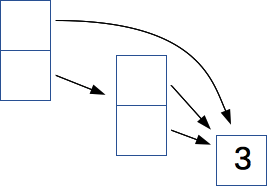
\includegraphics{fig/label.png}
\caption{Labelling}
\end{figure}
\end{quote}

\emph{Drawing diagrams} of things like data structures is also
straightforward to do on paper but very difficult to grade
automatically. One way to make solutions gradable may be to constrain
the drawing in the same way that Parsons Problems constrain code
construction, i.e., give students the pieces of the diagram and ask them
to arrange them correctly, but this is a long way off.

We mentioned earlier that matching problems require students to use
higher-order thinking skills. \emph{Summarization} also does this, and
gives them a chance to practice a skill that is very useful when
\emph{reporting} bugs rather than fixing them. For example, students can
be asked, ``Which sentence best describes how the output of f changes as
x varies from 0 to 10?'' and then given several options as a multiple
choice question. Similarly, ranking problems present the student with
several choices and ask them to order them from fastest to slowest, most
robust to most brittle, and so on. (Ranking is more manageable when
implemented with drag and drop than as a multiple choice question.)

One other kind of exercise that can be implemented as a multiple choice
question is \emph{fault mapping}: given a piece of buggy code and an
error message, the student has to identify the line on which the error
occurred. In simple cases this will be the line mentioned in the error
message, but in more subtle cases, the student will have to trace
execution forward and backward to figure out where things first went
wrong.

Other kinds of exercises are hard for any automated platform to provide.
\emph{Refactoring exercises} are the complement of theme and variation
exercises: given a working piece of code, the student has to modify it
in some way \emph{without} changing its output. For example, the student
could be asked to replace loops with vectorized expressions, to simplify
the condition in a while loop, etc. The challenge here is that there are
often so many ways to refactor a piece of code that grading requires
human intervention.

\begin{quote}
Example: write a single list comprehension that has the same effect as
this loop.

\begin{verbatim}
result = []
for v in values:
    if len(v) > threshold:
        result.append(v)
\end{verbatim}
\end{quote}

\emph{Code review} is hard to grade automatically in the general case,
but can be tackled if the student is given a rubric (i.e., a list of
faults to look for) and asked to match particular comments against
particular lines of code. For example, the student can be told that
there are two indentation errors and one bad variable name, and asked to
point them out; if she is more advanced, she could be given half a dozen
kinds of remarks she could make about the code without guidance as to
how many of each she should find. As with tracing values, this is
easiest for students to do when presented as a table, which we currently
don't support.

\begin{quote}
Example: using the rubric provided, mark each line of the code below.

\begin{verbatim}
01)  def addem(f):
02)      x1 = open(f).readlines()
03)      x2 = [x for x in x1 if x.strip()]
04)      changes = 0
05)      for v in x2:
06)          print('total', total)
07)          tot = tot + int(v)
08)      print('total')
\end{verbatim}

\begin{enumerate}
\def\labelenumi{\arabic{enumi}.}
\tightlist
\item
  poor variable name
\item
  unused variable
\item
  use of undefined variable
\item
  missing values
\item
  fossil code
\end{enumerate}
\end{quote}

All of this discussion has assumed that grading must be fully automatic
in order to scale to large classes, but that is not necessarily true.
{[}\href{biblio.html\#pare-joordens-peer}{Paré2008}{]} and
{[}\href{biblio.html\#kulkarni-peer-grading}{Kulkarni2013}{]} report
experiments in which learners grade each other's work, and the grades
they assign are then compared with grades given by graduate-level
teaching assistants or other experts. Both found that student-assigned
grades agreed with expert-assigned grades as often as the experts'
grades agreed with each other, and that a few simple steps (such as
filtering out obviously unconsidered responses or structuring rubrics)
decreased disagreement even further. Much more research needs to be
done, but given that critical reading is an effective way to learn, this
result may point to a future in which learners use technology to make
judgments, rather than being judged by technology.

\section{Challenges}\label{challenges-9}

\subsection{Give Feedback (20
minutes)}\label{give-feedback-20-minutes-1}

\begin{enumerate}
\def\labelenumi{\arabic{enumi}.}
\item
  Watch
  {[}\href{biblio.html\#wilson-bad-teaching-recorded}{Wilson2017}{]} as
  a group and give feedback on it. Organize feedback along two axes:
  positive vs.~negative and content vs.~presentation.
\item
  Have each person in the class add one point to a 2x2 grid on a
  whiteboard (or in the shared notes) without duplicating any points
  that are already up there.
\end{enumerate}

What did other people see that you missed? What did they think that you
strongly agree or disagree with?

\subsection{Adapting Multiple Choices Questions (30
minutes)}\label{adapting-multiple-choices-questions-30-minutes}

Pick one of the examples given in this chapter of using multiple choice
questions to implement some other kind of online programming exercise,
create an example, and swap with one of your fellow learners.

\subsection{Adapting Write and Run Exercises (30
minutes)}\label{adapting-write-and-run-exercises-30-minutes}

Pick one of the examples given in this chapter of using write and runs
exericses to implement some other kind of online programming exercise,
create an example, and swap with one of your fellow learners.

\chapter{Building Community}\label{building-community}

\begin{quote}
\textbf{Objectives}

\begin{itemize}
\tightlist
\item
  Learners can make an informed decision about whether to create
  something new, or join an existing effort.
\item
  Learners can judge whether a meeting is well organized and well run or
  not.
\item
  Learners can outline a three-step plan for recruiting, retaining, and
  retiring volunteers and other organization participants.
\item
  Learners can explain the difference between a service board and a
  governance board, and judge which kind an organization has.
\end{itemize}
\end{quote}

Many well-intentioned people want the world to be a better place, but
don't actually want anything important to change. A lot of grassroots
efforts to teach programming fall into this category: they want to teach
children and adults how to program so that they can get good jobs,
rather than empower them to change the system that has shut them (and
people like them) out of those jobs in the past.

If you are going to build a community, the first and most important
thing you have to decide is what \emph{you} want: to help people succeed
in the world we have, or to give them a way to make a better one. If you
choose the latter, you have to accept that one person can only do so
much. Just as we learn best together, we teach best when we are teaching
with other people, and the best way to achieve that is to build a
community.

\section{Learn, Then Do}\label{learn-then-do}

The first step in building a community is to decide if you really need
to, or whether you would be more effective joining an existing
organization. Thousands of groups are already teaching people tech
skills, from the \href{http://www.4-h-canada.ca/}{4-H Club} and
\href{https://www.frontiercollege.ca/}{literacy programs} to
get-into-coding non-profits like
\href{http://www.blackgirlscode.com/}{Black Girls Code}. Joining an
existing group will give you a head start on teaching, an immediate set
of colleagues, and a chance to learn more about how to run things. The
only thing it \emph{won't} give you is the ego gratification and control
that comes from being a founder.

Whether you join an existing group or set up one of your own, you owe it
to yourself and everyone who's going to work with you to find out what's
been done before. People have been writing about grassroots organizing
for decades; {[}\href{biblio.html\#alinsky-rules}{Alinsky1989}{]} is
probably the best-known work on the subject, while
{[}\href{biblio.html\#brown-bpco}{Brown2007}{]} and
{[}\href{biblio.html\#midwest-organizing}{Midwest2010}{]} are practical
manuals rooted in decades of practice. If you want to read more deeply,
{[}\href{biblio.html\#adams-seeds}{Adams1975}{]} is a history of the
Highlander Folk School, whose approach has been emulated by many
successful groups, while
{[}\href{biblio.html\#spalding-adults}{Spalding2014}{]} is a guide to
teaching adults written by someone with deep personal roots in
organizing.

\subsection{Meetings, Meetings,
Meetings}\label{meetings-meetings-meetings}

Knowing how to run a meeting efficiently is \emph{the} core skills of
community organizers. (Knowing how to take part in someone else's
meeting is just as important, but gets far less attention--as a
colleague once said, everyone offers leadership training, nobody offers
followership training.) The most important rules for making meetings
efficient are not secret, but are rarely followed:

\begin{enumerate}
\def\labelenumi{\arabic{enumi}.}
\item
  \emph{Decide if there actually needs to be a meeting.} If the only
  purpose is to share information, have everyone send a brief email
  instead.
\item
  \emph{Choose a chair.} A meeting without a chair is going to work just
  about as well as an orchestra without a conductor.
\item
  \emph{Write down the agenda, with timings.} List the items that are to
  be discussed and estimate the time allowed for each. Your first
  estimates with any new group will be wildly optimistic, so revise them
  upward for subsequent meetings.
\item
  \emph{No technology.} Insist that everyone put their phones, tablets,
  and laptops into politeness mode (i.e., closes them).
\item
  \emph{Record minutes.} Someone other than the chair should take
  point-form notes about the most important pieces of information that
  were shared, and about every decision that was made or every task that
  was assigned to someone.
\item
  \emph{Make sure the chair doesn't speak more than anyone else.} The
  chair is there to make sure that the meeting keeps moving, \emph{not}
  to do most of the talking.
\item
  \emph{Require politeness.} No one gets to interrupt anyone, no one
  gets to ramble, and if someone goes off topic, it's the chair's job to
  say, ``Let's discuss that elsewhere.''
\item
  \emph{End early.} If your meeting is scheduled for 10:00-11:00, you
  should aim to end at 10:55 to give people time to get where they need
  to go next.
\end{enumerate}

{[}\href{biblio.html\#brown-bpco}{Brown2007}{]} and
{[}\href{biblio.html\#brookfield-discussion}{Brookfield2016}{]} have
lots of good advice on running meetings, and if you want to ``learn,
then do'', an hour of training on chairing meetings is the most
effective place to start.

\begin{quote}
\textbf{Sticky Notes and Interruption Bingo}

Some people are so used to the sound of their own voice that they will
insist on talking half the time no matter how many other people are in
the room. One way to combat this is to give everyone three sticky notes
at the start of the meeting. Every time they speak, they have to take
down one sticky note. When they're out of notes, they aren't allowed to
speak until everyone has used at least one, at which point everyone gets
all of their sticky notes back. This ensures that nobody talks more than
three times as often as the quietest person in the meeting, and
completely changes the dynamics of most groups: people who have given up
trying to be heard because they always get trampled suddenly have space
to contribute, and the overly-frequent speakers quickly realize just how
unfair they have been.

Another useful technique is called interruption bingo. Draw a grid, and
label the rows and columns with the participants' names. Each time
someone interrupts someone else, add a tally mark to the appropriate
cell. Halfway through the meeting, take a moment to look at the results.
In most cases, you will see that one or two people are doing all of the
interrupting, often without being aware of it. After that, saying, ``All
right, I'm adding another tally to the bingo card,'' is often enough to
get them to throttle back.
\end{quote}

\section{Three Steps}\label{three-steps}

\begin{quote}
\begin{itemize}
\tightlist
\item
  Me in 2012: I'm not going to worry about retaining volunteers until I
  have a few.
\item
  My Dad: If you don't think about how you're going to keep them, you
  probably won't get any.
\end{itemize}
\end{quote}

Everyone who gets involved with your organization, including you, goes
through three phases: recruitment, retention, and retirement (from the
organization). You don't need to worry about this cycle when you're just
getting started, but it \emph{is} worth thinking about as soon as you
have more than a couple of non-founders involved.

The first step is recruiting volunteers. Your
\href{marketing.html}{marketing} should help you with this by making
your organization findable, and by making its mission and its value to
volunteers clear to people who might want to get involved. Share stories
that exemplify the kind of help you want as well as stories about the
people you're helping, and make it clear that there are many ways to get
involved. (We discuss this in more detail in the next section.)

Your best source of new recruits is your own classes: ``see one, do one,
teach one'' has worked well for volunteer organizations for as long as
there have \emph{been} volunteer organizations. Make sure that every
class or other encounter ends with two sentences explaining how people
can help, and that help is welcome. People who come to you this way will
know what you do, and will have recent experience of being on the
receiving end of what you offer that they can draw on, which helps your
organization avoid collective
\href{gloss.html\#expert-blind-spot}{expert blind spot}.

\begin{quote}
\textbf{Start Small}

As \href{https://en.wikipedia.org/wiki/Ben_Franklin_effect}{Ben
Franklin} observed, a person who has performed a favor for someone is
more likely to do another favor for that person than they would be if
they had received a favor from that person. Asking people to do
something small for you is therefore a good step toward getting them to
do something larger. One natural way to do this when teaching is to ask
people to submit fixes for your lesson materials for typos or unclear
wording, or to suggest new exercises or examples. If your materials are
written in a \href{lessons.html\#maintainability}{maintainable way},
this gives them a chance to practice some useful skills, and gives you
an opportunity to start a conversation that might lead to a new recruit.
\end{quote}

Recruiting doesn't end when someone first shows up: if you don't follow
through, people will come out once or twice, then decide that what
you're doing isn't for them and disappear. Two things you can do to get
newcomers over this initial hump are:

\begin{enumerate}
\def\labelenumi{\arabic{enumi}.}
\item
  Have them take part in group activities before they do anything on
  their own, both so that they get a sense of how your organization does
  things, and so that they build social ties that will keep them
  involved.
\item
  Give newcomers a mentor, and make sure the mentors actually do some
  proactive mentoring. The most important things a mentor can do are
  make introductions and explain the unwritten rules, so make it clear
  to mentors that these are their primary responsibilities, and they are
  to report back to you every few weeks to tell you what they've done.
\end{enumerate}

The second part of the volunteer lifecycle is retention, which is a
large enough topic to deserve its own section. The third and final part
is retirement. Sooner or later, everyone moves on (including you). When
this happens:

\begin{enumerate}
\def\labelenumi{\arabic{enumi}.}
\item
  Ask people to be explicit about their departure.
\item
  Make sure they don't feel embarrassed or ashamed about leaving.
\item
  Give them an opportunity to pass on their knowledge. For example, you
  can ask them to mentor someone for a few weeks as their last
  contribution, or to be interviewed by someone who's staying with the
  organization to collect any stories that are worth re-telling.
\item
  Make sure they hand over the keys. It's awkward to discover six months
  after someone has left that they're the only person who knows how to
  book a playing field for the annual softball game.
\item
  Follow up 2-3 months after they leave to see if they have any further
  thoughts about what worked and what didn't while they were with you,
  or any advice to offer that they either didn't think to give or were
  uncomfortable giving on their way out the door.
\item
  Thank them, both when they leave and the next time your group gets
  together.
\end{enumerate}

\section{Retention}\label{retention}

The community organizer Saul Alinksy said, ``If your people aren't
having a ball doing it, there is something very wrong.'' Community
members shouldn't expect to enjoy every moment of their work with your
organization, but if they don't enjoy any of it, they won't stay.

Enjoyment doesn't necessarily mean having an annual party: people may
enjoy cooking, coaching, or just working quietly beside others. There
are several things every organization should do to ensure that people
are getting something they value out of their work:

\begin{enumerate}
\def\labelenumi{\arabic{enumi}.}
\item
  \emph{Ask people what they want rather than guessing.} Just as
  \href{lesson.html\#a-reminder}{you are not your learners}, you are
  probably different from other members of your organization. Ask people
  what they want to do, what they're comfortable doing (which may not be
  the same thing), what constraints there are on their time, and so on.
\item
  \emph{Provide many ways to contribute.} The more ways there are for
  people to help, the more people will be able to help. Someone who
  doesn't like standing in front of an audience may be able to maintain
  your organization's website or handle its accounts; someone who
  doesn't know how to do anything else may be able to proof-read
  lessons, and so on. The more kinds of tasks you do yourself, the fewer
  opportunities there are for others to get involved.
\item
  \emph{Recognize contributions.} Everyone likes to be appreciated, so
  communities should acknowledge their members' contributions both
  publicly and privately.
\item
  \emph{Make space.} Micromanaging or trying to control everything
  centrally means people won't feel they have the autonomy to act, which
  will probably cause them to drift away. In particular, if you're too
  engaged or too quick on the reply button, people have less opportunity
  to grow as members and to create horizontal collaborations. The
  community can continue to be ``hub and spoke'', focused around one or
  two individuals, rather than a highly-connected network in which
  others feel comfortable participating.
\end{enumerate}

Another way to make participation rewarding is to provide training.
Organizations require committees, meetings, budgets, grant proposals,
and dispute resolution; most people are never taught how to do any of
this, any more than they are taught how to teach, but training people to
do these things helps your organization run more smoothly, and the
opportunity to gain transferable skills is a powerful reason for people
to get and stay involved. If you are going to do this, don't try to
provide the training yourself (unless it's what you specialize in). Many
civic and community groups have programs of this kind, and you can
probably make a deal with one of them.

Other groups may be useful in other ways as well, and you may be useful
to them--if not immediately, then tomorrow or next year. You should
therefore set aside an hour or two every month to find allies and
maintain your relationships with them. One way to do this is to ask them
for advice: how do they think you ought to raise awareness of what
you're doing? Where have they found space to run classes? What needs do
they think aren't being met, and would you be able to meet them (either
on your own, or in partnership with them)? Any group that has been
around for a few years will have useful advice; they will also be
flattered to be asked, and will know who you are the next time you call.

\begin{quote}
\textbf{Government Matters}

Have you ever spoken to someone from the public relations office at your
local college or school board, or in your city councilor's office? If
not, what are you waiting for?
\end{quote}

\begin{quote}
\textbf{Soup, Then Hymns}

Manifestos are fun to write, but most people join a volunteer community
to help and be helped rather than to argue over the wording of a grand
vision statement. (Most people who prefer the latter are \emph{only}
interested in arguing\ldots{}) To be effective you should therefore
focus on things that are immediately useful, e.g., on what people can
create that will be used by other community members right away. Once
your organization shows that it can actually achieve things--even small
things--people will be more confident that it's worth thinking about
bigger issues.
\end{quote}

One important special case of making things rewarding is to pay people.
Volunteers can do a lot, but eventually tasks like system administration
and accounting need full-time paid staff. This is often a difficult
transition for grassroots organizations, but is outside the scope of
this book.

\section{Governance}\label{governance}

As Jo Freeman pointed out in her influential essay
``\href{http://www.jofreeman.com/joreen/tyranny.htm}{The Tyranny of
Structurelessness}'', every organization has a power structure: the only
question is whether it's formal and accountable, or informal and
unaccountable. Make yours one of the first kind: write and publish the
rules governing everything from who's allowed to use the name and logo
to who gets to decide whether people are allowed to charge money to
teach with whatever materials your group has worked up.

Organizations can govern themselves in many different ways, and a full
discussion of the options is outside the scope of this book. The most
important thing to keep in mind is that countries and corporations are
only two of many governance models, and that a commons is often a better
model for volunteer teaching organizations. A commons is ``something
managed jointly by a community according to rules they themselves have
evolved and adopted''; as
{[}\href{biblio.html\#bollier-commoner}{Bollier2014}{]} emphasizes, all
three parts of that definition are essential: a commons isn't just a
shared pasture, but also includes the community that shares it and the
rules they use to do so.

Most resources, throughout most of human history, have been commons: it
is only in the last few hundred years that impersonal markets have
pushed them to the margins. In order to do so, free-market advocates
have had to convince us we're something we're not (dispassionate
calculators of individual advantage) and erase or devalue local
knowledge and custom. Both have had tragic consequences for us
individually and communally, and now for our whole planet.

Since society has difficulty recognizing commons organizations, and
since most of the people you will want to recruit don't have experience
with them, you will probably wind up having some sort of board, a
director, and other staff. Broadly speaking, your organization can have
either a \emph{service board}, whose members also take on other roles in
the organization, or a \emph{governance board} whose primary
responsibility is to hire, monitor, and if need be fire the director.
Board members can be elected by the community or appointed; in either
case, it's important to prioritize competence over passion (the latter
being more important for the rank and file), and to try to recruit for
particular skills such as accounting, marketing, and so on.

Don't worry about drafting a constitution when you first get started: it
will only result in endless wrangling about what we're going to do
rather than formalization of what you're already doing. When the time
does come to formalize your rules, though, make your organization a
democracy: sooner or later (usually sooner), every appointed board turns
into a mutual agreement society and loses sight of what the community
it's meant to serve actually needs. Giving the community power is messy,
but is the only way invented so far to ensure that an organization
continues to meet people's actual needs.

\section{Final Thoughts}\label{final-thoughts}

As {[}\href{biblio.html\#pigni-idealists}{Pigni2016}{]} discusses,
burnout is a chronic risk in any community activity. If you don't take
care of yourself, you won't be able to take care of your community.

Every organization eventually needs fresh ideas and fresh leadership.
When that time comes, train your successors and then move on. They will
undoubtedly do things you wouldn't have, but the same is true of every
generation. Few things in life are as satisfying as watching something
you helped build take on a life of its own. Celebrate that--you won't
have any trouble finding something else to keep you busy.

\section{Challenges}\label{challenges-10}

Several of these exercises are taken from
{[}\href{biblio.html\#brown-bpco}{Brown2007}{]}, which is an
exceptionally useful book on building community organizations.

\subsection{Who Are You? (15 minutes)}\label{who-are-you-15-minutes}

Which of the descriptions of people you don't want on your team do you
fit? What can you do about it?

\subsection{People You May Meet (30
minutes)}\label{people-you-may-meet-30-minutes}

As an organizer, part of your job is sometimes to help people find a way
to contribute despite themselves. In small groups, pick three of the
people below and discuss how you would help them become a better
contributor to your organization.

\begin{itemize}
\item
  \emph{Anna} knows more about every subject than everyone else put
  together--at least, she thinks she does. No matter what you say,
  she'll correct you; no matter what you know, she knows better.
\item
  \emph{Catherine} has so little confidence in her own ability that she
  won't make any decision, no matter how small, until she has checked
  with someone else.
\item
  \emph{Frank} believes that knowledge is power, and enjoys knowing
  things that other people don't. He can make things work, but when
  asked how he did it, he'll grin and say, ``Oh, I'm sure you can figure
  it out.''
\item
  \emph{Hediyeh} is quiet. She never speaks up in meetings, even when
  she knows that what other people are saying is wrong. She might
  contribute to the mailing list, but she's very sensitive to criticism,
  and will always back down rather than defending her point of view.
  Hediyeh isn't a troublemaker, but rather a lost opportunity.
\item
  \emph{Kenny} has discovered that most people would rather shoulder his
  share of the work than complain about him, and he takes advantage of
  it at every turn. The frustrating thing is that he's so damn
  \emph{plausible} when someone finally does confront him. ``There have
  been mistakes on all sides,'' he says, or, ``Well, I think you're
  nit-picking.''
\item
  \emph{Melissa} means well, but somehow something always comes up, and
  her tasks are never finished until the last possible moment. Of
  course, that means that everyone who is depending on her can't do
  their work until \emph{after} the last possible moment\ldots{}
\item
  \emph{Raj} is rude. ``It's just the way I talk,'' he says, ``If you
  can't hack it, maybe you should find another team.'' His favorite
  phrase is, ``That's stupid,'' and he uses obscenity as casually as
  minor characters in Tarantino films.
\end{itemize}

\subsection{Values (45 minutes)}\label{values-45-minutes}

Answer the following questions on your own, and then compare your
answers to those given by other members of your group.

\begin{enumerate}
\def\labelenumi{\arabic{enumi}.}
\tightlist
\item
  What are the values your organization expresses?
\item
  Are these the values you want the organization to express?
\item
  If not, what values would you like it to express?
\item
  What are the specific behaviors that demonstrate those values?
\item
  What are some key behaviors that would demonstrate the values you
  would like for your group?
\item
  What are the behaviors that would demonstrate the opposite of those
  values?
\item
  What are some key behaviors that would demonstrate the opposite of the
  values you want to have?
\end{enumerate}

\subsection{Meeting Procedures (30
minutes)}\label{meeting-procedures-30-minutes}

Answer the following questions on your own, and then compare your
answers to those given by other members of your group.

\begin{enumerate}
\def\labelenumi{\arabic{enumi}.}
\tightlist
\item
  How are your meetings run?
\item
  Is this how you want your meetings to be run?
\item
  Are the rules for running meetings explicit or just assumed?
\item
  Are these the rules you want?
\item
  Who is eligible to vote/make decisions?
\item
  Is this who you want to be vested with decision-making authority?
\item
  Do you use majority rule, make decisions by consensus, or use some
  other method?
\item
  Is this the way you want to make decisions?
\item
  How do people in a meeting know when a decision has been made?
\item
  How do people who weren't at a meeting know what decisions were made?
\item
  Is this working for your group?
\end{enumerate}

\subsection{Size (20 minutes)}\label{size-20-minutes}

Answer the following questions on your own, and then compare your
answers to those given by other members of your group.

\begin{enumerate}
\def\labelenumi{\arabic{enumi}.}
\tightlist
\item
  How big is your group?
\item
  Is this the size you want for your organization?
\item
  If not, what size would you like it to be?
\item
  Do you have any limits on the size of membership?
\item
  Would you benefit from setting such a limit?
\end{enumerate}

\subsection{Staffing (30 minutes)}\label{staffing-30-minutes}

Answer the following questions on your own, and then compare your
answers to those given by other members of your group.

\begin{enumerate}
\def\labelenumi{\arabic{enumi}.}
\tightlist
\item
  Do you have paid staff in your organization?
\item
  Or is it all-volunteer?
\item
  Should you have paid staff?
\item
  Do you want/need more or less staff?
\item
  What do you call the staff (e.g., organizer, director, coordinator,
  etc.)?
\item
  What do the staff members do?
\item
  Are these the primary roles and functions that you want the staff to
  be filling?
\item
  Who supervises your staff?
\item
  Is this the supervision process and responsibility chain that you want
  for your group?
\item
  What is your staff paid?
\item
  Is this the right salary to get the needed work done and to fit within
  your resource constraints?
\item
  What benefits does your group provide to its staff (health, dental,
  pension, short and long-term disability, vacation, comp time, etc.)?
\item
  Are these the benefits that you want to give?
\end{enumerate}

\subsection{Collaborations (30
minutes)}\label{collaborations-30-minutes}

Answer the following questions on your own, and then compare your
answers to those given by other members of your group.

\begin{enumerate}
\def\labelenumi{\arabic{enumi}.}
\tightlist
\item
  Do you have any agreements or relationships with other groups?
\item
  Do you want to have relationships with any other groups?
\item
  How would having (or not having) collaborations help you to achieve
  your goals?
\item
  What are your key collaborative relationships?
\item
  Are these the right collaborators for achieving your goals?
\item
  With what groups or entities would you like your organization to have
  agreements or relationships?
\end{enumerate}

\subsection{Money (30 minutes)}\label{money-30-minutes}

Answer the following questions on your own, and then compare your
answers to those given by other members of your group.

\begin{enumerate}
\def\labelenumi{\arabic{enumi}.}
\tightlist
\item
  Who pays for what?
\item
  Is this who you want to be paying?
\item
  Where do you get your money?
\item
  Is this how you want to get your money?
\item
  If not, do you have any plans to get it another way?
\item
  If so, what are they?
\item
  Who is following up to make sure that happens?
\item
  How much money do you have?
\item
  How much do you need?
\item
  What do you spend most of your money on?
\item
  Is this how you want to spend your money?
\end{enumerate}

\subsection{Becoming a Member (45
minutes)}\label{becoming-a-member-45-minutes}

Answer the following questions on your own, and then compare your
answers to those given by other members of your group.

\begin{enumerate}
\def\labelenumi{\arabic{enumi}.}
\tightlist
\item
  How does someone join?
\item
  Does this process work for your organization?
\item
  What are the membership criteria?
\item
  Are these the membership criteria you want?
\item
  Are people required to agree to any rules of behavior upon joining?
\item
  Are these the rules for behavior you want?
\item
  Are there membership dues?
\end{enumerate}

\chapter{Marketing}\label{marketing}

\begin{quote}
\textbf{Objectives}

\begin{itemize}
\tightlist
\item
  Learners can explain what marketing actually is.
\item
  Learners can clearly explain the value of what they are offering to
  different potential stakeholders.
\item
  Learners can explain what a brand is and determine whether they or
  their organization have one.
\end{itemize}
\end{quote}

It's hard to get people with technical backgrounds to think about
marketing, not least because it's perceived as being about spin and
misdirection. In reality, \emph{\href{gloss.html\#marketing}{marketing}}
is the craft of seeing things from other people's perspective,
understanding their wants and needs, and finding ways to meet them. This
should sound familiar: many of the techniques introduced earlier in this
book are intended to do exactly this for lessons. This chapter will look
at how to apply similar ideas to the larger problem of getting people to
support the work you're trying to do.

\section{What Are You Offering to
Whom?}\label{what-are-you-offering-to-whom}

The first step is to figure out what you are offering to whom, i.e.,
what actually brings in the funding and other support you need to keep
operating. As {[}\href{biblio.html\#kuchner-marketing}{Kuchner2011}{]}
points out, the answer is often counter-intuitive. For example, most
scientists think their product is papers, but their actual product is
their grant proposals, because those are what brings in money. Their
papers are the advertising that persuades people to buy (fund) those
proposals, just as albums are now the advertising that persuades people
to buy musicians' concert tickets and t-shirts.

You may or may not be a scientist, so suppose instead that your group is
offering weekend programming workshops to people who are re-entering the
workforce after taking several years out to look after young children.
If your learners are paying enough for your workshops to cover your
costs, then the learners are your customers and the workshops are the
product. If, on the other hand, the workshops are free, or the learners
are only paying a token amount (to cut the no-show rate), then your
actual product may be some mix of:

\begin{itemize}
\tightlist
\item
  your grant proposals,
\item
  the alumni of your workshops that the companies sponsoring you would
  like to hire,
\item
  the half page summary of your work in the mayor's annual report to
  city council that shows how she's supporting the local tech sector, or
\item
  the personal satisfaction that teaching gives your volunteer
  instructors.
\end{itemize}

As with our \href{design.html}{recommended lesson design process}, you
should try to identify specific people who might be interested in what
you're doing and figure out which of \emph{their} needs \emph{your}
program will meet. \href{lessons.html\#learner-personas}{Personas} are
one way to do this. Another is to write a set of
\emph{\href{gloss.html\#elevator-pitch}{elevator pitches}}, each aimed
at a different stakeholder. A widely-used template for these pitches
looks like this:

For

target audience

who

dissatisfaction with what's currently available

our

category

provide

key benefit.

Unlike

alternatives

our program

key distinguishing feature

Continuing with our weekend workshop example, we might use this for
potential attendees:

\begin{quote}
For \emph{people re-entering the workforce after taking time out to
raise children} who \emph{still have regular childcare
responsibilities}, our \emph{introductory programming workshops} provide
\emph{weekend classes with on-site childcare}. Unlike \emph{online
classes}, our program \emph{gives participants a chance to meet people
who are at the same stage of life}.
\end{quote}

but use this to characterize the companies that we would like to donate
staff time for teaching:

\begin{quote}
For \emph{a company that wants to recruit entry-level software
developers} that \emph{is struggling to find mature, diverse candidates}
our \emph{introductory programming workshops} provide \emph{a pool of
potential recruits in their thirties that includes large numbers of
people from underrepresented groups}. Unlike \emph{college recruiting
fairs}, our program \emph{connects companies directly with a diverse
audience}.
\end{quote}

If you don't know why different potential stakeholders might be
interested in what you're doing, ask them. If you do know, ask them
anyway: answers can change over time, and it's a good way to discover
things that you might have missed. Once you have written these pitches,
you should use them to drive what you put on your organization's web
site and in other publicity material, since it will help people figure
out as quickly as possible whether you and they have something to talk
about. However, you probably \emph{shouldn't} copy them verbatim, since
many people in tech have seen this template so often that their eyes
will glaze over if they encounter it again.

As you are writing these pitches, remember that people are not just
economic animals. A sense of accomplishment, control over their own
lives, and being part of a community motivates them just as much as
money. People may volunteer to teach with you because it's what their
friends are doing; similarly, a company may say that they're sponsoring
classes for economically disadvantaged high school students because they
want a larger pool of potential employees further down the road, but in
reality, the CEO might actually be doing it simply because it's the
right thing to do.

\section{Branding and Positioning}\label{branding-and-positioning}

A \emph{\href{gloss.html\#brand}{brand}} is someone's first reaction to
a mention of a product; if their reaction is ``what's that?'', you don't
have a brand yet. Branding is important because people aren't going to
help with something they don't know about or don't care about.

Most discussion of branding today focuses on ways to build awareness
online. Mailing lists, blogs, and Twitter all give you ways to reach
people, but as the volume of (mis)information steadily increases, the
attention paid to any particular interruption decreases. As this
happens, \emph{\href{gloss.html\#positioning}{positioning}} becomes more
important. Positioning (sometimes also called ``differentiation'') is
what sets your offering apart from others: it's the ``unlike'' section
of your elevator pitches. When you are reaching out to people who are
already generally familiar with your field, this is what you should
emphasize, since it's what will catch their attention.

There are other things you can do to help build your brand as well. One
is to use props: a robot car that one of your students made from scraps
she found around the house, the website another student made for his
parents' retirement home, or anything else that makes what you're doing
seem real. Another is to make a short video--no more than a few minutes
long--showcasing the backgrounds and accomplishments of your students.
The aim of both is to tell a story: while people always ask for data,
stories are what they believe.

\begin{quote}
\textbf{Foundational Myths}

One of the most compelling stories a person or organization can tell is
about why and how they got started. Are you teaching what you wish
someone had taught you but didn't? Was there one particular person you
wanted to help, and that opened the floodgates? Are you picking up where
someone else left off, and if so, why?
\end{quote}

Free samples are also compelling. Put some lesson materials online so
that people can see what you teach; post a few (short) videos from
actual workshops, or go to where your hoped-for learners or sponsors are
and run a lunchtime drop-in session.

Whatever else you do, make your organization findable by doing what you
can to make you and your organization rank highly in Google searches.
There's a lot of folklore about how to do this under the label ``SEO''
(for ``search engine optimization''); given Google's near-monopoly
powers and lack of transparency, most of it boils down to trying to stay
one step ahead of algorithms designed to prevent people from gaming
rankings. Search for yourself and for your organization on a regular
basis and see what comes up, then read
\href{https://moz.com/learn/seo/on-page-factors}{these guidelines from
Moz} and do what you can to improve your site. Keep
\href{https://xkcd.com/773/}{this cartoon} in mind: people don't
(initially) want to know about your org chart or get a virtual tour of
your site; they want your address, parking information, and above all,
some idea of what you teach, when you teach it, how to get in touch, and
how it's going to change their life.

Offline findability is equally important for new organizations. Many of
the people you hope to reach might not be online, or might not be online
as often as you; notice boards in schools, local libraries, drop-in
centers, and grocery stores are still an effective way to reach them.

\begin{quote}
\textbf{Build Alliances}

As discussed in the \href{community.html}{previous chapter}, building
alliances with other groups that are doing things related to what you're
doing pays off in many ways. One of those is referrals: if someone
approaches you for help, but would be better served by some other
organization, take a moment to make an introduction. If you've done this
several times, add something to your website to help the next person
find what they need. The organizations you are helping will soon start
to help you in return.
\end{quote}

\section{The Art of the Cold Call}\label{the-art-of-the-cold-call}

Building a web site and hoping that people find it is one thing; calling
people up or knocking on their door without any sort of prior
introduction is another. As with standing up and teaching, though, it's
a craft that can be learned like any other, and there are a few simple
rules you can follow:

\begin{enumerate}
\def\labelenumi{\arabic{enumi}.}
\item
  Start by establishing a point of connection: ``I was speaking to X''
  or ``You attended bootcamp Y''. This must be specific: spammers and
  headhunters have trained us all to ignore anything that starts, ``I
  recently read your website''.
\item
  Explain how you are going to help make their lives better (e.g.,
  ``Your students will be able to do their math homework much faster if
  you let us help them'').
\item
  Be specific about what you are offering (e.g., ``Our usual two-day
  curriculum includes\ldots{}'') so that they can figure out right away
  whether this is worth pursuing, but keep it to one or two sentences.
\item
  Mention your backers, your size, how long you've been around, or your
  instructors's backgrounds to make yourself credible.
\item
  Create a slight sense of urgency (``we're booking workshops right
  now'').
\item
  Tell them what your terms are: do you charge money, do they need to
  cover instructors' travel costs, can they reserve seats for their own
  staff, etc.
\item
  Above all, \emph{keep it short}. The message below takes 30 seconds or
  less to scan; by the end, either they're interested enough to reply or
  they're not.
\end{enumerate}

This template works pretty well, but ``pretty well'' is relative. Most
organizations expect a 2-3\% response rate to cold calls; for Software
Carpentry, we found that about half of emails were answered, about half
of those answers were, ``Sure, let's talk more,'' and about half of
those led to workshops, which means that 10-15\% of targeted emails to
people we had some sort of connection with turned into workshops.

\begin{quote}
\textbf{Mail Out of the Blue}

Hi {[}name{]},

I hope you don't mind mail out of the blue, but I wanted to follow up on
our conversation at the tech showcase last week to see if you would be
interested having us run a Software Carpentry workshop for your graduate
students. We're scheduling workshops for the coming year right now, and
it might be a way to help them accelerate their research.

Software Carpentry's aim is to teach graduate students and other
researchers the basic computing skills they need to get more done in
less time and with less pain. Our usual two-day curriculum includes:

\begin{itemize}
\item
  the Unix shell (but we're really teaching them how to automate
  repetitive tasks);
\item
  Git and GitHub (but we're really teaching them how to use version
  control to track and share their work);
\item
  Python or R (but we're really teaching them how to grow a program in a
  structured, modular, testable, reusable way); and
\item
  databases (but we're really teaching them the difference between
  structured and unstructured data).
\end{itemize}

Our instructors are volunteers, so the only cost to host sites is their
travel and accommodation plus a \$1500 contribution toward central costs
like instructor training and curriculum development. We aim for 40
people per workshop, and look for 2-3 local helpers to assist during
practicals.

We've run hundreds of workshops like this in 34 countries since 2010,
and several assessments have confirmed that what we're doing actually
helps. If this sounds interesting, please give me a shout.

Thanks for your time, Dr.~Greg Wilson
\end{quote}

\section{Go Over, Go Through, Go Around, or Change
Direction}\label{go-over-go-through-go-around-or-change-direction}

Everyone is afraid of the unknown and of embarrassing themselves. As a
result, most people would rather fail than change. Marketing is
therefore not just about communicating clearly: it is also about
figuring out why people are resisting your offer of help and then
finding a way past that resistance.

For example, Lauren Herckis looked at
\href{https://www.insidehighered.com/news/2017/07/06/anthropologist-studies-why-professors-dont-adopt-innovative-teaching-methods}{why
university faculty don't adopt better teaching methods}. She found that
the main reason is a fear of looking stupid in front of their students,
and that secondary reasons were concern that the inevitable bumps in
switching how they taught would affect course evaluations, and a desire
to continue emulating the lecturers who had inspired them. It's
pointless to argue about whether these issues are ``real'' in some
objective sense: faculty believe they are, so any marketing aimed at
faculty needs to address them.

Medical researchers realized several decades ago that there's no point
coming up with a better way to do things if practitioners won't adopt
it. The growing field of
\emph{\href{gloss.html\#implementation-science}{implementation science}}
explores evidence-based ways to improve transference, and
{[}\href{biblio.html\#borrego-henderson-change}{Borrego2014}{]}
categories some related ideas for effecting change in higher education.
The bulk of that paper expands upon this table (which is included as an
image because rotating text in a simple cross-browser fashion is
apparently still beyond present-day technology):

\begin{figure}
\centering
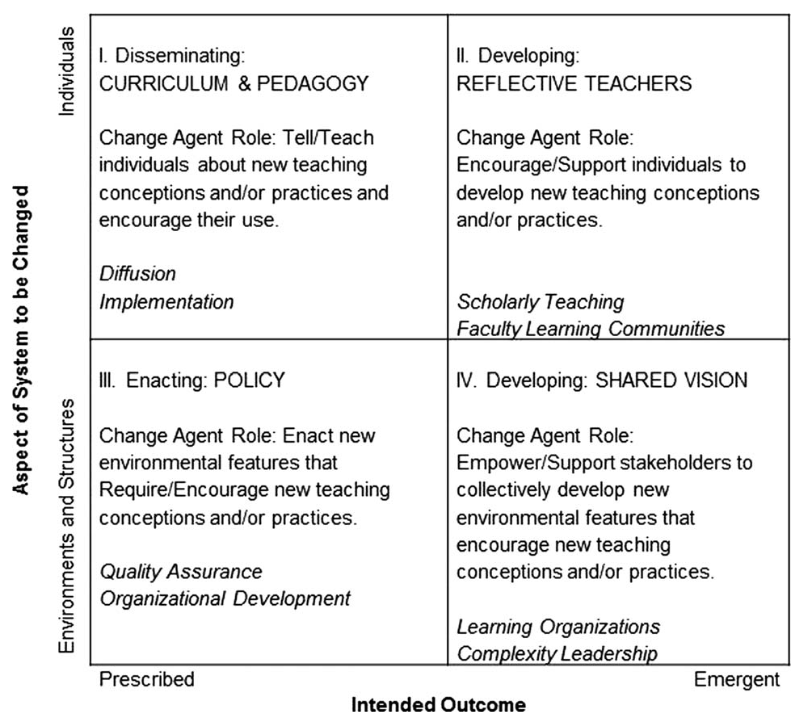
\includegraphics{fig/borrega-henderson-table.png}
\caption{Change in Higher Education}
\end{figure}

Each of the major categories is defined by whether the change is
individual or to the system as a whole, and whether it is prescribed
(top-down) or emergent (bottom-up). The person trying to make the
changes--and make them stick--has a different role in each situation,
and should pursue different strategies accordingly.

\section{A Final Thought}\label{a-final-thought}

As {[}\href{biblio.html\#kuchner-marketing}{Kuchner2011}{]} says, if you
can't be first in a category, create a new category that you can be
first in; if you can't do that, think about doing something else
entirely. This isn't as defeatist as it sounds: if someone else is
already doing what you're doing better than you, there are probably lots
of other equally useful things you could be doing instead.

\section{Challenges}\label{challenges-11}

\subsection{Write an Elevator Pitch for a City Councilor (15
minutes)}\label{write-an-elevator-pitch-for-a-city-councilor-15-minutes}

This chapter described an organization that offers weekend programming
workshops for people re-entering the workforce after taking a break to
raise children. Write an elevator pitch for that organization aimed at a
city councilor whose support the organization needs.

\subsection{Write Elevator Pitches for Your Organization (30
minutes)}\label{write-elevator-pitches-for-your-organization-30-minutes}

Identify two groups of people your organization needs support from, and
write an elevator pitch aimed at each one.

\subsection{Identify Causes of Passive Resistance (30
minutes)}\label{identify-causes-of-passive-resistance-30-minutes}

People who don't want change will sometimes say so out loud, but will
also often use various forms of passive resistance, such as just not
getting around to it over and over again, or raising one possible
problem after another to make the change seem riskier and more expensive
than it's actually likely to be. Working in small groups, list three or
four reasons why people might not want your teaching initiative to go
ahead, and explain what you can do with the time and resources you have
to counteract each.

\chapter{License}\label{license}

This work is licensed under the Creative Commons Attribution 3.0
Unported license (CC-BY-3.0). You are free:

\begin{itemize}
\tightlist
\item
  to Share--to copy, distribute and transmit the work
\item
  to Remix--to adapt the work
\end{itemize}

\noindent
under the following conditions:

\begin{itemize}
\tightlist
\item
  Attribution--you must attribute the work in the manner specified by
  the author or licensor (but not in any way that suggests that they
  endorse you or your use of the work).
\end{itemize}

\noindent
with the understanding that:

\begin{itemize}
\item
  Waiver--Any of the above conditions can be waived if you get
  permission from the copyright holder.
\item
  Public Domain--Where the work or any of its elements is in the public
  domain under applicable law, that status is in no way affected by the
  license.
\item
  Other Rights--In no way are any of the following rights affected by
  the license:

  \begin{itemize}
  \tightlist
  \item
    Your fair dealing or fair use rights, or other applicable copyright
    exceptions and limitations;
  \item
    The author's moral rights;
  \item
    Rights other persons may have either in the work itself or in how
    the work is used, such as publicity or privacy rights.
  \end{itemize}
\item
  Notice--For any reuse or distribution, you must make clear to others
  the license terms of this work. The best way to do this is with a link
  to \url{http://creativecommons.org/licenses/by/3.0/}.
\end{itemize}

\chapter{Code of Conduct}\label{code-of-conduct}

\begin{quote}
To ensure a welcoming environment for all, we require everyone
participating in our classes to conform to the Code of Conduct given
below. This code applies to all spaces managed by our group including,
but not limited to, workshops, mailing lists, and online forums
(including source code repositories). We strongly recommend that anyone
running workshops or classes of any kind choose and publish a similar
code so that everyone will know what is expected of them and what to do
when those expectations are not met.
\end{quote}

We are dedicated to providing a welcoming and supportive environment for
all people, regardless of background or identity. However, we recognize
that some groups in our community are subject to historical and ongoing
discrimination, and may be vulnerable or disadvantaged. Membership in
such a specific group can be on the basis of characteristics such as
such as gender, sexual orientation, disability, physical appearance,
body size, race, nationality, sex, color, ethnic or social origin,
pregnancy, citizenship, familial status, veteran status, genetic
information, religion or belief, political or any other opinion,
membership of a national minority, property, birth, age, or choice of
text editor. We do not tolerate harassment of participants on the basis
of these categories, or for any other reason.

Harassment is any form of behavior intended to exclude, intimidate, or
cause discomfort. Because we are a diverse community, we may have
different ways of communicating and of understanding the intent behind
actions. Therefore we have chosen to prohibit certain forms of behavior
in our community, regardless of intent. Prohibited harassing behavior
includes but is not limited to:

\begin{itemize}
\item
  written or verbal comments which have the effect of excluding people
  on the basis of membership of a specific group listed above;
\item
  causing someone to fear for their safety, such as through stalking,
  following, or intimidation;
\item
  the display of sexual or violent images;
\item
  unwelcome sexual attention;
\item
  non-consensual or unwelcome physical contact;
\item
  sustained disruption of talks, events or communications;
\item
  incitement to violence, suicide, or self-harm;
\item
  continuing to initiate interaction (including photography or
  recording) with someone after being asked to stop; and
\item
  publication of private communication without consent.
\end{itemize}

Behavior not explicitly mentioned above may still constitute harassment.
The list above should not be taken as exhaustive but rather as a guide
to make it easier to enrich all of us and the communities in which we
participate. All interactions should be professional regardless of
location: harassment is prohibited whether it occurs on or offline, and
the same standards apply to both.

Enforcement of the Code of Conduct will be respectful and not include
any harassing behaviors.

Thank you for helping make this a welcoming, friendly community for all.

\emph{This code of conduct is a modified version of that used by PyCon,
which in turn is forked from a template written by the Ada Initiative
and hosted on the Geek Feminism Wiki.}

\chapter{Citation}\label{citation}

Please cite this work as:

\vspace*{\baselineskip}

\noindent
Greg Wilson (ed.): \emph{How to Teach Programming (And Other Things)}.
Second edition, Lulu.com, 2017, 978-1-365-98428-0,
\url{http://third-bit.com/teaching}.

\chapter{How to Contribute}\label{how-to-contribute}

We welcome contributions of all kinds, from errata to suggestions for
improvements to new material. The source for this book is stored in a
GitHub repository at \url{http://github.com/gvwilson/thirdbit.git}, so
if you know how to use Git, and would like to add or fix something,
please send us a pull request.

If you don't know how to use Git, you can file an issue in that
repository or email the editor at \texttt{gvwilson@third-bit.com}.
Please note that by doing so, you are agreeing that we may incorporate
your changes in either original or edited form and release them under
the same \href{/license/}{license} as the rest of this material. Please
also note that we require everyone involved in this project to abide by
our \href{conduct.html}{Code of Conduct}.

Finally, we are always grateful to hear how you have used this material
and how we could make it better: please email us if you have a story you
would like to share.

\chapter{Extra Material}\label{extra-material}

This section includes material that doesn't naturally fit anywhere else.

\section{How to Use This Material}\label{how-to-use-this-material}

This material has been taught as a multi-week online class, as a two-day
in-person class, and as a two-day class in which the learners are in
co-located groups and the instructor participates remotely.

\begin{quote}
\textbf{Terminology}

When we talk about workshops, we will try to be clear about whether
we're discussing ones whose subject is programming, which are aimed at
general learners, and those whose subject is how to teach, which are
using this material.
\end{quote}

\subsection{In-Person}\label{in-person}

In our experience, this is the most effective way to deliver an
instructor training workshop.

\begin{itemize}
\item
  Participants are physically together for one or two days. When they
  need to work in small groups (e.g., for practice teaching), some or
  all of them go to nearby breakout spaces. Participants bring their own
  tablets or laptops to view and edit online material during the class,
  and use pen and paper and/or whiteboards for some exercises.
\item
  Participants use Etherpad or Google Doc for in-person training, both
  for \href{practices.html\#take-notes-together}{shared note-taking} and
  for posting exercise solutions and feedback on recorded lessons.
  Questions and discussion are done aloud.
\item
  Several times during the training, participants are put in groups of
  three to teach for 2-3 minutes. The mechanics are described
  \href{performance.html\#how-to-practice-teaching}{later}, and while
  participants are initially intimidated at first, they routinely rank
  it as the most useful part of the class.
\end{itemize}

\subsection{Two-Day Online With
Groups}\label{two-day-online-with-groups}

In this format, learners are in groups of 4-12, but those groups are
geographically distributed.

\begin{itemize}
\item
  Each class uses an Etherpad or Google Doc for
  \href{practices.html\#take-notes-together}{shared note-taking}, and
  more importantly for asking and answering questions: having several
  dozen people try to talk on a call works poorly, so in most sessions,
  the instructor does the talking and learners respond through the
  note-taking tool's chat.
\item
  Each group of learners is together in a room using one camera and
  microphone, rather than each being on the call separately. We have
  found that having good audio matters more than having good video, and
  that the better the audio, the more learners can communicate with the
  instructor and other rooms by voice rather than by using the Etherpad
  chat.
\item
  We do the video lecture exercise as in the two-day in-person training.
\end{itemize}

\subsection{Multi-Week Online}\label{multi-week-online}

This was the first format we used, and we no longer recommend it.

\begin{itemize}
\item
  We met every week or every second week for an hour via web
  conferencing. Each meeting was held twice (or even three times) to
  accommodate learners' time zones and because video conferencing
  systems can't handle 60+ people at once.
\item
  We used web conferencing and shared note-taking as described above for
  online group classes.
\item
  Learners posted homework online between classes, and commented on each
  other's work. (In practice, comments were relatively rare: people
  seemed to prefer to discuss material in the web chats.)
\item
  We used a WordPress blog for the first ten rounds of training, then a
  GitHub-backed blog, and finally Piazza. WordPress worked best: setting
  up accounts was tedious, but everything after that ran smoothly. Using
  a GitHub blog worked so poorly that we didn't try it again: a third of
  the participants found it extremely frustrating, and post-publication
  commentary was awkward. Piazza was better than GitHub, but still not
  as easy for participants to pick up as WordPress. In particular, it
  was hard to find things once there were more than a dozen homework
  categories.
\end{itemize}

\section{Key Terms}\label{key-terms}

\emph{\href{gloss.html\#educational-psychology}{Educational psychology}}
is the study of how people learn. It touches on everything from the
neuropsychology of perception and the mechanisms of memory to the
sociology of school systems and the philosophical question of what we
actually mean by ``learning'' (which turns out to be pretty complicated
once you start looking beyond the standardized Western classroom).
Within the broad scope of educational psychology, two specific
perspectives have primarily influenced our teaching practices (and by
extension, this instructor training).

The first perspective is
\emph{\href{gloss.html\#cognitivism}{cognitivism}}, which treats
learning as a problem in neuropsychology. Cognitivists focus their
attention on things like pattern recognition, memory formation, and
recall. It is good at answering low-level questions, but generally
ignores larger issues like, ``What do we mean by `learning'?'' and,
``Who gets to decide?''

The second perspective is
\emph{\href{gloss.html\#situated-learning}{situated learning}}, which we
discussed in \href{community.html}{Building Community}. For example,
Software Carpentry aims to serve researchers who are exploring data
management and programming on their own (legitimate peripheral practice)
and make them aware of other people doing that work (simply by attending
the workshop) and the best practices and ideas of that community of
practice, thereby giving them a way to become members of that community.
Situated learning thus describes why we teach, and recognizes that
teaching and learning are always rooted in a social context. We then
depend on the cognitivist perspective to drive \emph{how} we teach the
specific content associated with the community of practice.

\begin{quote}
\textbf{Other Perspectives}

There are many other perspectives outside cognitivist theory---see the
Learning Theories site
{[}\href{biblio.html\#learning-theories}{Learning2017}{]} for summaries.
Besides cognitivism, those encountered most frequently include
\emph{\href{gloss.html\#behaviorism}{behaviorism}} (which treats
education as stimulus/response conditioning),
\emph{\href{gloss.html\#constructivism}{constructivism}} (which
considers learning an active process during which learners construct
knowledge for themselves), and
\emph{\href{gloss.html\#connectivism}{connectivism}} (which emphasizes
the social aspects of learning, particularly those made possible by the
Internet). And yes, it would help if their names were less
similar\ldots{}
\end{quote}

Educational psychology does not tell us how to teach on its own because
it under-constrains the problem: in real life, several different
teaching methods might be consistent with what we currently know about
how learning works. We therefore have to try those methods in the class,
with actual learners, in order to find out how well they balance the
different forces in play.

Doing this is called
\emph{\href{gloss.html\#instructional-design}{instructional design}}. If
educational psychology is the science, instructional design is the
engineering. For example, there are good reasons to believe that
children will learn how to read best by starting with the sounds of
letters and working up to words. However, there are equally good reasons
to believe that children will learn best if they are taught to recognize
entire simple words like ``open'' and ``stop'', so that they can start
using their knowledge sooner.

The first approach is called ``phonics'', and the second, ``whole
language''. The whole language approach may seem upside down, but more
than a billion people have learned to read and write Chinese and similar
ideogrammatic languages in exactly this way. The only way to tell which
approach works best for most children, most of the time, is to try them
both out. These studies have to be done carefully, because so many other
variables can have an impact on rules. For example, the teacher's
enthusiasm for the teaching method may matter more than the method
itself, since children will model their teacher's excitement for a
subject.

Unsurprisingly, effective teaching depends on what the teacher knows,
which can be divided into:

\begin{itemize}
\item
  \emph{\href{gloss.html\#content-knowledge}{content knowledge}}, such
  as the ``what'' of programming;
\item
  \emph{\href{gloss.html\#general-pedagogical-knowledge}{general
  pedagogical knowledge}}, i.e., an understanding of the psychology of
  learning; and
\item
  the \emph{\href{gloss.html\#pedagogical-content-knowledge}{pedagogical
  content knowledge}} (PCK) that connects the two. PCK is things like
  what examples to use when teaching how parameters are passed to a
  function, or what misconceptions about wildcard expansion are most
  common. For example, an instructor could write variable names and
  values on paper plates and then stack and unstack them to show how the
  call stack works.
\end{itemize}

A great example of PCK is
{[}\href{biblio.html\#gelman-stats}{Gelman2002}{]}, which is full of PCK
for teaching introductory statistics. The CS Teaching Tips site
{[}\href{biblio.html\#cs-teaching-tips}{Tips2017}{]} is gathering
similar ideas for computing.

\section{Situated Learning}\label{situated-learning}

A framework in which to think about grassroots education is
\emph{\href{gloss.html\#situated-learning}{situated learning}}, which
focuses on how
\emph{\href{gloss.html\#legitimate-peripheral-participation}{legitimate
peripheral participation}} leads to people becoming members of a
\emph{\href{gloss.html\#community-of-practice}{community of practice}}.
Unpacking those terms, a community of practice is a group of people
bound together by interest in some activity, such as knitting or
particle physics. Legitimate peripheral participation means doing
simple, low-risk tasks that community nevertheless recognizes as valid
contributions: making your first scarf, stuffing envelopes during an
election campaign, or proof-reading documentation for open source
software.

Situated learning focuses on the transition from being a newcomer to
being accepted as a peer by those who are already community members.
This typically means starting with simplified tasks and tools, then
doing similar tasks with more complex tools, and finally tackling the
challenges of advanced practitioners. For example, children learning
music may start by playing nursery rhymes on a recorder or ukulele, then
play other simple songs on a trumpet or saxophone in a band, and finally
start exploring their own musical tastes. Healthy communities understand
and support these progressions, and recognize that each step is meant to
give people a ramp rather than a cliff.

Whatever the domain, situated learning emphasizes that learning is a
social activity. In order to be effective and sustainable, teaching
therefore needs to be rooted in a community; if one doesn't exist, you
need to build one.

\section{Myths}\label{myths}

One
\href{https://en.wikipedia.org/wiki/Learning_styles\#Learning_modalities}{well-known
scheme} characterizes learners as visual, auditory, or kinesthetic
according to whether they like to see things, hear things, or do things.
This scheme is easy to understand, but as de Bruyckere and colleagues
point out in \emph{Urban Myths About Learning and Education}
{[}\href{biblio.html\#debruyckere-urban-myths}{DeBruyckere2015}{]}, it
is almost certainly false. Unfortunately, that hasn't stopped a large
number of companies from marketing products based on it to parents and
school boards.

This is not the only myth to plague education. The learning pyramid that
shows we remember 10\% of what we read, 20\% of what we hear, and so on?
Myth. The idea that ``brain games'' can improve our intelligence, or at
least slow its decline in old age? Also a myth, as are the claims that
the Internet is making us dumber or that young people read less than
they used to.

Computing education has its own myths. Mark Guzdial's ``Top 10 Myths
About Teaching Computer Science''
{[}\href{biblio.html\#guzdial-top10}{Guzdial2015a}{]} are:

\begin{enumerate}
\def\labelenumi{\arabic{enumi}.}
\item
  The lack of women in Computer Science is just like all the other STEM
  fields.
\item
  To get more women in CS, we need more female CS faculty.
\item
  A good CS teacher is a good lecturer.
\item
  Clickers and the like are an add-on for a good teacher.
\item
  Student evaluations are the best way to evaluate teaching.
\item
  Good teachers personalize education for students' learning styles.
\item
  High schools just can't teach CS well, so they shouldn't do it at all.
\item
  The real problem is to get more CS curriculum into the hands of
  teachers.
\item
  All I need to do to be a good CS teacher is model good software
  development practice, because my job is to produce excellent software
  engineers.
\item
  Some people are just born to program.
\end{enumerate}

The last of these is the most pervasive and most damaging. As discussed
in \href{motivation.html}{Motivation}, Elizabeth Patitsas and others
have shown that grades in computing classes are \emph{not} bimodal
{[}\href{biblio.html\#patitsas-cs-grades}{Patitsas2016}{]}, i.e., there
isn't one group that gets it and another that doesn't. Many of the
participants in our workshops have advanced degrees in intellectually
demanding subjects, but have convinced themselves that they just don't
have what it takes to be programmers. If all we do is dispel that
belief, we will have done them a service.

\section{Feedback on Bad Teaching Demo
Videos}\label{feedback-on-bad-teaching-demo-videos}

The two lists below summarize key feedback on the videos of
\href{biblio.html\#wilson-bad-teaching-live}{bad live teaching} and
\href{biblio.html\#wilson-bad-teaching-recorded}{bad recorded teaching}
used in the chapters on \href{performance.html}{performance} and
\href{online.html}{online teaching}.

\subsection{Part 1: Bad Teaching in
Person}\label{part-1-bad-teaching-in-person}

\begin{itemize}
\tightlist
\item
  Starts by being rude to audience (``Could you sit down? Yeah, now
  please.'')
\item
  Text on the screen is far too small.
\item
  Speaker frequently interrupts himself.
\item
  Uses nonsensical names like ``foo'' instead of authentic tasks.
\item
  First example returns the type of its argument: again, not a common
  task.
\item
  ``This is really simple stuff - even Excel users can understand it.''
  Don't denigrate people's existing knowledge.
\item
  ``This is instantiating a new function object.'' Too much unnecessary
  jargon.
\item
  ``Yes, and it's lexical binding.''
\item
  ``Which of course is polymorphic.''
\item
  ``And as you'd expect from something which is doing lazy binding on
  types.''
\item
  ``It works like you'd expect.'' No it doesn't--it took some of the
  brightest minds of the 20th Century several decades to come up with
  our current model of computing. To suggest otherwise is to imply that
  people who don't already understand it are stupid.
\item
  ``Trust me.'' Never a good thing to hear a teacher say\ldots{}
\item
  01:29 check phone. The audience will never care more about the
  material than the presenter, and it's pretty clear at this point that
  the presenter doesn't care a lot.
\item
  01:40 defining higher-level functions.
\item
  Any audience that needed basic function definition explained won't be
  ready for this.
\item
  Any audience that's ready for this didn't need basic functions
  defined.
\item
  Conclusion: the presenter has no idea who his audience actually is.
\item
  02:01 Corrected the mistake without explaining it.
\item
  Failed to turn the mistake into a teachable moment.
\item
  Will leave audience confused: what was wrong and why?
\end{itemize}

\subsection{Part 2: Bad Teaching in Recorded
Video}\label{part-2-bad-teaching-in-recorded-video}

\begin{itemize}
\tightlist
\item
  Clipped at the start: normally start talking about a second in to give
  people a chance to collect themselves.
\item
  Flubbed the first sentence: don't do a hundred takes, but don't just
  do one either.
\item
  Screen is very cluttered: several irrelevant background windows open.
\item
  Terminal is very cluttered: what does all that text have to do with
  the lesson?
\item
  Font is much too small.
\item
  Flipped between windows at 00:15 for no apparent reason.
\item
  Speaking far too quickly.
\item
  Starts by talking about some other platform that isn't on the screen,
  rather than what is.
\item
  Don't draw attention at 00:30 to the Python version unless it's
  important.
\item
  Background noise at 00:40.
\item
  Explanation of what functions are seems to trying to motivate the
  lesson, but:
\item
  uses jargon like ``parameterize'',
\item
  nothing is happening on the screen while the presenter is talking, and
\item
  reference to previous courses the learner might have done are
  obviously improvised.
\item
  Audio is garbed starting at 01:16.
\item
  Closing the background windows at 1:33 just draws attention to them at
  this point.
\item
  Typing in code starting at 01:52 introduces a lot of background noise
  (keyboard clicking).
\item
  ``And it takes some sort of parameter'' introduces important jargon
  (parameter), but then the presenter talks about the colon instead.
\item
  Presenter goes from ``body'' to ``scoping'' starting at 2:07 without
  any clear explanation.
\item
  Then dives down a rabbit hole briefly discussing scoping rules: this
  will be unintelligible to anyone new to functions.
\item
  02:28 ``to get back to a top-level prompt'' - what's a ``top-level
  prompt''?
\item
  At least the presenter is using a meaningful name for the
  function\ldots{}
\item
  02:43 ``this is all pretty simple stuff'' - no! It's only simple once
  you know it.
\item
  02:50 ``even if all you know is something like R'': don't denigrate
  people's existing knowledge, or other communities.
\item
  Pasting in a block of code around 03:05
\item
  The code isn't explained\ldots{}
\item
  \ldots{}and nobody is going to be able to keep up with the speed.
\item
  03:11 more background noise
\item
  03:12 Since there is a built-in function called `sum', use some other
  name for the example function to avoid confusion.
\item
  03:18 ``Because we've got to write something'': the audience will
  never care more about the material than the presenter, and it's pretty
  clear at this point that the presenter doesn't care a lot.
\item
  03:22 ``Let me just rewrite this because we haven't introduced
  variable arguments.''
\item
  What bug is the presenter fixing?
\item
  What are ``variable arguments''? (Remember, this is the viewer's first
  introduction to functions.)
\item
  The replacement code is identical to the original code except for one
  '*' character: beginners aren't going to notice that or know why it's
  important.
\item
  03:34 more keyboard clicking.
\item
  03:40 background voices.
\item
  03:53 ``This is so simple, even Excel users could follow along.''
  Again, never be derogatory in a lesson.
\item
  04:02 ``This is actually polymorphic on types.'' Presenter clearly has
  no audience level in mind.
\item
  Anyone who is new to functions isn't going to understand what
  ``polymorphic on types'' means.
\item
  04:09 Summing `a', `b', and `c' fails.
\item
  Don't include failing examples in videos unless the failure is
  purposeful.
\item
  If a failure is included, explain what the fault was and how it was
  fixed (more than ``I can't initialize\ldots{}'' and then
  self-interruption).
\item
  04:18 Abandoning example and going back to `double' is going to
  confuse viewers.
\item
  04:40 Explanation of why doubling `x' produces `xx' is garbled and has
  nothing to do with functions.
\item
  04:48 ``As you'd probably expect, you can nest the function calls'':
  there are many things that are more important to explain before nested
  function calls.
\item
  04:58 ``Yeah, I guess that's right.'' Does not inspire confidence in
  the presenter.
\item
  05:13 Audio is garbled again.
\item
  05:34 List comprehensions are another distraction.
\item
  Last few seconds should have been edited out.
\end{itemize}

\section{Feedback on Live Coding Demo
Videos}\label{feedback-on-live-coding-demo-videos}

The two lists below summarize key feedback on the two videos used in the
discussion of \href{live.html}{live coding}.

\subsection{Part 1: How Not to Do It}\label{part-1-how-not-to-do-it}

\begin{itemize}
\item
  Instructor ignores a red sticky clearly visible on a learner's laptop.
\item
  Instructor is sitting, mostly looking at the laptop screen.
\item
  Instructor is typing commands without saying them out loud.
\item
  Instructor uses fancy shell prompt in the console window.
\item
  Instructor uses small font in not full-screen console window with
  black background.
\item
  The console window bottom is partially blocked by the learner's heads
  for those sitting in the back.
\item
  Instructor receives a a pop-up notification in the middle of the
  session.
\item
  Instructor makes a mistake (a typo) but simply fixes it without
  pointing it out, and redoes the command.
\end{itemize}

\subsection{Part 2: How to Do It Right}\label{part-2-how-to-do-it-right}

\begin{itemize}
\item
  Instructor checks if the learner with the red sticky on her laptop
  still needs attention.
\item
  Instructor is standing while instructing, making eye-contact with
  participants.
\item
  Instructor is saying the commands out loud while typing them.
\item
  Instructor moves to the screen to point out details of commands or
  results.
\item
  Instructor simply uses \texttt{\$} as shell prompt in the console
  window.
\item
  Instructor uses big font in wide-screen console window with white
  background.
\item
  The console window bottom is above the learner's heads for those
  sitting in the back.
\item
  Instructor makes mistake (a typo) and uses the occasion to illustrate
  how to interpret error-messages.
\end{itemize}

\section{Effecting Change}\label{effecting-change}

This guide is aimed primarily at people working in grassroots
organizations, but in order to reach and help as many people as
possible, we must find ways to work with the schools we have.
{[}\href{biblio.html\#henderson-facilitating}{Henderson2011}{]}
discusses ways to get educational institutions to change what and how
they teach; in our experience, the most important things are:

\begin{enumerate}
\def\labelenumi{\arabic{enumi}.}
\item
  \emph{Ask, don't tell.} Teachers know their students and their needs
  much better than you do, so start by asking what they think the most
  pressing needs are.
\item
  \emph{Find allies.} Many colleges and universities have teaching and
  learning centers whose staff are keen to improve teaching practices,
  and who also know how to navigate the local bureaucracy. Similarly,
  there are often tech meetup groups or other local organizations whose
  members are likely helpers.
\item
  \emph{Start small.}
  {[}\href{biblio.html\#lang-small-teaching}{Lang2016}{]} describes
  evidence-based teaching practices that can be put in place with
  minimal effort and at low cost. These may not have the most impact,
  but scoring a few early wins helps build support for larger and
  riskier efforts.
\end{enumerate}

{[}\href{biblio.html\#brown-bpco}{Brown2007}{]} is an excellent guide to
building organizations in and for communities. You may not need to
answer all of the questions it asks right away, but they are all worth
thinking about.

\section{Evaluating Impact}\label{evaluating-impact}

A key part of effecting change is to convince people that what you're
doing is having a positive impact. That turns out to be surprisingly
hard for free-range programming workshops:

\begin{enumerate}
\def\labelenumi{\arabic{enumi}.}
\item
  \emph{Ask learners if the workshop was useful.} Study after study has
  shown that there is no correlation between how highly learners rate a
  course and how much they actually learn
  {[}\href{biblio.html\#uttl-evaluations}{Uttl2016}{]}, and most people
  working in education are now aware of that.
\item
  \emph{Give them an exam at the end of the workshop.} Doing that
  dramatically changes the feel of the workshop, and how much they know
  at the end of the day is a poor predictor of how much they will
  remember two or three months later.
\item
  \emph{Give them an exam two or three months later.} That's hard enough
  to do in a traditional battery-farmed learning environment; doing it
  with free-range learners is even harder. In addition:

  \begin{itemize}
  \item
    The people who didn't get anything out of the workshop are probably
    less likely to take part in follow-up, so feedback gathered this way
    will be subject to self-selection bias.
  \item
    The fact that learners \emph{remember} something doesn't necessarily
    mean it was useful (although they are more likely to remember things
    that are useful than things that aren't).
  \end{itemize}
\item
  \emph{See if they keep using what they learned.} This is a good way to
  evaluate employment-oriented skills, but equally useful for things
  people have learned for fun. The problem is how to do it: you probably
  shouldn't put spyware on their computers, and follow-up surveys suffer
  from the same low return rate and self-selection bias as exams.
\item
  \emph{See if they recommend the workshop to friends.} This method
  often strikes the best balance between informative and doable: if
  people are recommending your workshop to other people, that's a pretty
  good sign.
\end{enumerate}

There are many other options; the most important thing is to figure out
early on how you're going to know whether you're teaching the right
things the right way, and how you're going to convince potential backers
that you're doing so.

\section{Three Kinds of Thinking}\label{three-kinds-of-thinking}

{[}\href{biblio.html\#fink-significant}{Fink2013}{]} suggests designing
exercises to prompt three kinds of thinking, and provides these examples
(among others):

\begin{verbatim}
<th>Field</th>
<th>Critical Thinking</th>
<th>Creative Thinking</th>
<th>Practical Thinking</th>
\end{verbatim}

\begin{verbatim}
<td>Biology</td>
<td>Evaluate the validity of the bacterial theory of ulcers.</td>
<td>Design a experiment to test the bacterial theory of ulcers.</td>
<td>How would the bacterial theory of ulcers change conventional treatment regimes?</td>
\end{verbatim}

\begin{verbatim}
<td>Art</td>
<td>Compare and contrast how Rembrandt and Van Gogh used light in these two paintings.</td>
<td>Draw a beam of light.</td>
<td>How could we reproduce the lighting in this painting in an actual room?</td>
\end{verbatim}

To ensure that key concepts are truly understood, instructors should
give learners exercises of all three types for each concept.

\chapter{Bibliography}\label{bibliography}

\section{What to Read Next}\label{what-to-read-next}

\begin{itemize}
\item
  \protect\hypertarget{ambrose-hlw}{}{{[}Ambrose2010{]}} Susan A.
  Ambrose, Michael W. Bridges, Michele DiPietro, Marsha C. Lovett, and
  Marie K. Norman:
  \emph{\href{https://www.amazon.com/How-Learning-Works-Research-Based-Principles/dp/0470484101/}{How
  Learning Works: Seven Research-Based Principles for Smart Teaching}}
  Jossey-Bass, 2010, 978-0470484104. \emph{An excellent overview of what
  we know about education and why we believe it's true, covering
  everything from cognitive psychology to social factors.}
\item
  \protect\hypertarget{brookfield-discussion}{}{{[}Brookfield2016{]}}
  Stephen D. Brookfield and Stephen Preskill:
  \emph{\href{https://www.amazon.com/Discussion-Book-Great-People-Talking/dp/1119049717/}{The
  Discussion Book: 50 Great Ways to Get People Talking}} Jossey-Bass,
  2016, 978-1119049715. \emph{Describes fifty different ways to get
  groups talking productively.}
\item
  \protect\hypertarget{brown-bpco}{}{{[}Brown2007{]}} Michael Jacoby
  Brown:
  \emph{\href{https://www.amazon.com/Building-Powerful-Community-Organizations-Personal/dp/0977151808/}{Building
  Powerful Community Organizations}} Long Haul Press, 2007,
  978-0977151806. \emph{An excellent practical introduction to creating
  effective organizations in and for communities written by someone with
  decades of experience doing exactly that.}
\item
  \protect\hypertarget{didau-teachers-psych}{}{{[}Didau2016{]}} David
  Didau and Nick Rose:
  \emph{\href{https://www.amazon.com/Every-Teacher-Needs-About-Psychology/dp/1909717851/}{What
  Every Teacher Needs to Know About Psychology}} John Catt Educational,
  2016, 978-1909717855. \emph{An informative, opinionated survey of what
  modern psychology has to say about teaching.}
\item
  \protect\hypertarget{green-babt}{}{{[}Green2014{]}} E. Green:
  \emph{\href{https://www.amazon.com/Building-Better-Teacher-Teaching-Everyone/dp/0393351084/}{Building
  a Better Teacher: How Teaching Works (and How to Teach It to
  Everyone)}} W. W. Norton, 2014, 978-0393244151. \emph{A well-written
  look at why educational reforms in the past 50 years have mostly
  missed the mark, and what we should be doing instead.}
\item
  \protect\hypertarget{guzdial-lcd}{}{{[}Guzdial2015b{]}} Mark Guzdial:
  \_\href{https://www.amazon.com/Learner-Centered-Design-Computing-Education-Human-Centered/dp/1627053514/}{Learner-Centered
  Design of Computing Education: Research on Computing for Everyone}
  Morgan \& Claypool, 2015, 978-1627053518. \emph{An evidence-based
  argument that we must design computing education for everyone, not
  just people who think they are going to become professional
  programmers.}
\item
  \protect\hypertarget{huston-dont-know}{}{{[}Huston2009{]}} Therese
  Huston:
  \emph{\href{https://www.amazon.com/Teaching-What-You-Dont-Know/dp/0674035801/}{Teaching
  What You Don't Know}} Harvard University Press, 2009, 978-0674035805.
  \emph{A pointed, funny, and very useful book that explores exactly
  what the title suggests.}
\item
  \protect\hypertarget{lang-small-teaching}{}{{[}Lang2016{]}} James M.
  Lang:
  \emph{\href{https://www.amazon.com/Small-Teaching-Everyday-Lessons-Learning/dp/1118944496/}{Small
  Teaching: Everyday Lessons from the Science of Learning}} Jossey-Bass,
  2016, 978-1118944493. \emph{Presents a selection of accessible
  evidence-based practices that teachers can adopt when they little time
  and few resources.}
\item
  \protect\hypertarget{lemov-champion}{}{{[}Lemov2014{]}} Doug Lemov:
  \emph{\href{https://www.amazon.com/Teach-Like-Champion-2-0-Techniques/dp/1118901851/}{Teach
  Like a Champion 2.0: 62 Techniques that Put Students on the Path to
  College}} (2nd edition). Jossey-Bass, 2014, 978-1118901854.
  \emph{Presents 62 classroom techniques drawn from intensive study of
  thousands of hours of video of good teachers in action.}
\item
  \protect\hypertarget{margolis-fisher-clubhouse}{}{{[}Margolis2003{]}}
  J. Margolis and A. Fisher:
  \emph{\href{https://www.amazon.com/Unlocking-Clubhouse-Women-Computing-Press/dp/0262632691/}{Unlocking
  the Clubhouse: Women in Computing}} MIT Press, 2003, 978-0262632690.
  \emph{A groundbreaking report on the gender imbalance in computing,
  and the steps Carnegie-Mellon took to address the problem.}
\end{itemize}

\section{Other References}\label{other-references}

\begin{itemize}
\item
  \protect\hypertarget{abela-chart}{}{{[}Abela2009{]}} Andrew Abela:
  ``Chart Suggestions--A Thought Starter''.
  \url{http://extremepresentation.typepad.com/files/choosing-a-good-chart-09.pdf},
  viewed April 2017.
\item
  \protect\hypertarget{ada-imposter}{}{{[}Ada2017{]}} Ada Initiative:
  ``Imposter Syndrome training''.
  \url{https://adainitiative.org/continue-our-work/impostor-syndrome-training/},
  viewed May 2017.
\item
  \protect\hypertarget{adams-seeds}{}{{[}Adams1975{]}} {Frank Adams:
  \emph{\href{https://www.amazon.com/Unearthing-Seeds-Fire-Idea-Highlander/dp/0895870193/}{Unearthing
  Seeds of Fire: The Idea of Highlander}}. John F. Blair, 1975,
  978-0895870193. \emph{A history of the Highlander Folk School and its
  founder, Myles Horton, who inspired many other social change
  organizations.}}
\item
  \protect\hypertarget{aiken-note-taking}{}{{[}Aiken1975{]}} Edwin G.
  Aiken, Gary S. Thomas, and William A. Shennum: ``Memory for a Lecture:
  Effects of Notes, Lecture Rate, and Informational Density.''
  \emph{Journal of Educational Psychology}, 67(3), June 1975,
  10.1037/h0076613. \emph{A landmark study showing that taking notes
  improves retention when learning.}
\item
  \protect\hypertarget{alinsky-rules}{}{{[}Alinsky1989{]}} {Saul
  Alinsky:
  \emph{\href{https://www.amazon.com/Rules-Radicals-Practical-Primer-Realistic/dp/0679721134/}{Rules
  for Radicals: A Practical Primer for Realistic Radicals}} Vintage,
  1989, 978-0679721130. \emph{A widely-read guide to community
  organization written by one of the 20th Century's great organizers.}}
\item
  \protect\hypertarget{video-peer-instruction}{}{{[}Avanti2013{]}}:
  Avanti Learning Centre: ``ConcepTests at Avanti's Learning Centre in
  Kanpur.'' \url{https://www.youtube.com/watch?v=2LbuoxAy56o}, viewed
  April 2017.
\item
  \protect\hypertarget{aveling-checklists}{}{{[}Aveling2013{]}}
  Emma-Louise Aveling, Peter McCulloch, and Mary Dixon-Woods: ``A
  Qualitative Study Comparing Experiences of the Surgical Safety
  Checklist in Hospitals in High-Income and Low-Income Countries.''
  \emph{BMJ Open}, 3(8), 2013, 10.1136/bmjopen-2013-003039.
  \emph{Reports on surgical checklist implementations and effects in the
  UK and Africa.}
\item
  \protect\hypertarget{barker-practice-adoption}{}{{[}Barker2015{]}}
  Lecia Barker, Christopher Lynnly Hovey, and Jane Gruning: ``What
  Influences CS Faculty to Adopt Teaching Practices?'', \emph{Proc. 46th
  ACM Technical Symposium on Computer Science Education}, 2015,
  10.1145/2676723.2677282. \emph{Describes findings from a two-part
  study of how computer science educators adopt new teaching practices.}
\item
  \protect\hypertarget{benner-expertise}{}{{[}Benner2000{]}} Patricia
  Benner:
  \emph{\href{https://www.amazon.com/Novice-Expert-Excellence-Clinical-Commemorative/dp/0130325228/}{From
  Novice to Expert: Excellence and Power in Clinical Nursing Practice}}
  Pearson, 2000, 978-0130325228. \emph{A classic study of clinical
  judgment and how expertise develops.}
\item
  \protect\hypertarget{biggs-tang-quality}{}{{[}Biggs2011{]}} {John
  Biggs and Catherine Tang:
  \emph{\href{https://www.amazon.com/Teaching-Learning-University-Research-Education/dp/0335242758/}{Teaching
  for Quality Learning at University}} Open University Press, 2011,
  978-0335242757. \emph{A step-by-step guide to lesson development,
  delivery, and evaluation for people working in higher education.}}
\item
  \protect\hypertarget{bohay-note-taking}{}{{[}Bohay2011{]}} Mark Bohay,
  Daniel P. Blakely, Andrea K. Tamplin, and Gabriel A. Radvansky: ``Note
  Taking, Review, Memory, and Comprehension.'' \emph{American Journal of
  Psychology}, 124(1), 2011, 10.5406/amerjpsyc.124.1.0063.
  \emph{Presents a study showing that note-taking improves retention
  most at deeper levels of understanding.}
\item
  \protect\hypertarget{bollier-commoner}{}{{[}Bollier2014{]}} {David
  Bollier:
  \emph{\href{https://www.amazon.com/Think-Like-Commoner-Introduction-Commons/dp/0865717680/}{Think
  Like a Commoner: A Short Introduction to the Life of the Commons}} New
  Society Publishers, 2014, 978-0865717688. \emph{A short introduction
  to one of the most widely used kinds of governance in human societies
  throughout history.}}
\item
  \protect\hypertarget{borrego-henderson-change}{}{{[}Borrego2014{]}}
  Maura Borrego and Charles Henderson: ``Increasing the Use of
  Evidence-Based Teaching in STEM Higher Education: A Comparison of
  Eight Change Strategies.'' \emph{Journal of Engineering Education},
  103(2), April 2014, 10.1002/jee.20040. \emph{Categories different
  approaches to effecting change in higher education.}
\item
  \protect\hypertarget{brown-empirical}{}{{[}Brown2014{]}} Neil C. C.
  Brown and Amjad Altadmri: ``Investigating Novice Programming Mistakes:
  Educator Beliefs vs.~Student Data.'' \emph{Proc Tenth Annual
  Conference on International Computing Education Research}, 2014,
  10.1145/2632320.2632343. \emph{Uses data from over 100,000 students to
  show that educators know less than they think about what mistakes
  novice programmers actually make.}
\item
  \protect\hypertarget{cottom-lower-ed}{}{{[}Cottom{]}} {Tressie
  McMillan Cottom:
  \emph{\href{https://www.amazon.com/Lower-Ed-Troubling-Profit-Colleges/dp/1620970600/}{Lower
  Ed: The Troubling Rise of For-Profit Colleges in the New Economy}} The
  New Press, 2017, 978-1620970607. \emph{Lays bare the dynamics of this
  growing ``educational'' industry to show how it leads to greater
  inequality rather than less.}}
\item
  \protect\hypertarget{cottrill-gifted}{}{{[}Cottrill2016{]}} Cameron
  Cottrill: ``Why Talented Black and Hispanic Students Can Go
  Undiscovered.''
  \url{https://mobile.nytimes.com/2016/04/10/upshot/why-talented-black-and-hispanic-students-can-go-undiscovered.html},
  viewed April 2017.
\item
  \protect\hypertarget{deathbulge-feedback-feeling}{}{{[}Deathbulge
  Feedback Feelings{]}} Deathbulge: ``Feedback Feelings''.
  \url{http://www.deathbulge.com/comics/155}, viewed May 2017. \emph{How
  many of us react to feedback.}
\item
  \protect\hypertarget{debruyckere-urban-myths}{}{{[}DeBruyckere2015{]}}
  Pedro De Bruyckere, Paul A. Kirschner, and Casper D. Hulshof:
  \emph{\href{https://www.amazon.com/Urban-Myths-about-Learning-Education/dp/0128015373/}{Urban
  Myths about Learning and Education}} Academic Press, 2015,
  978-0128015377. \emph{Describes and debunks some widely-held myths
  about how people learn.}
\item
  \protect\hypertarget{epstein-thinking-physics}{}{{[}Epstein2002{]}}
  L.C. Epstein:
  \emph{\href{https://www.amazon.com/Thinking-Physics-Understandable-Practical-Reality/dp/0935218084/}{Thinking
  Physics is Gedanken Physics}} Insight Press, 2002: 978-0935218084.
  \emph{An entertaining problem-based introduction to thinking like a
  physicist.}
\item
  \protect\hypertarget{ericson-parsons}{}{{[}Ericson2017{]}} {Barbara J.
  Ericson, Lauren E. Margulieux, and Jochen Rick: ``Solving Parsons
  Problems Versus Fixing and Writing Code.'' Proc. Koli Calling 2017,
  November 2017, 10.1145/3141880.3141895. \emph{Another in a series of
  studies showing that Parsons Problems are an effective way to teach
  programming.}}
\item
  \protect\hypertarget{fehily-sql}{}{{[}Fehily2008{]}} Chris Fehily:
  \emph{\href{https://www.amazon.com/SQL-Visual-QuickStart-Guide-3rd/dp/0321553578/}{SQL:
  Visual QuickStart Guide}} (3rd edition). Peachpit Press, 2008
  978-0321553577. \emph{An introduction to SQL that is both a good
  tutorial and a good reference guide.}
\item
  \protect\hypertarget{fincher-stories-change}{}{{[}Fincher2012{]}}
  Sally Fincher, Brad Richards, Janet Finlay, Helen Sharp, and Isobel
  Falconer: ``Stories of Change: How Educators Change Their Practice.''
  \emph{Proc. Frontiers in Education Conference}, 2012,
  10.1109/FIE.2012.6462317. \emph{A detailed look at how educators
  actually adopt new teaching practices.}
\item
  \protect\hypertarget{fincher-warrens-questions}{}{{[}Fincher2007{]}}
  Sally Fincher and Josh Tenenberg: ``Warren's Question.'' \emph{Proc.
  Third International Workshop on Computing Education Research}, 2007,
  10.1145/1288580.1288588. \emph{A detailed look at a particular
  instance of transferring a teaching practice.}
\item
  \protect\hypertarget{fink-short}{}{{[}Fink2003{]}} L. Dee Fink: ``A
  Self-Directed Guide to Designing Courses for Significant Learning.''
  \url{https://www.deefinkandassociates.com/GuidetoCourseDesignAug05.pdf},
  viewed April 2017.
\item
  \protect\hypertarget{fink-significant}{}{{[}Fink2013{]}} L. Dee Fink:
  \emph{\href{https://www.amazon.com/Creating-Significant-Learning-Experiences-Integrated/dp/1118124251/}{Creating
  Significant Learning Experiences: An Integrated Approach to Designing
  College Courses}} (2nd edition). Jossey-Bass, 2013, 978-1118124253.
  \emph{A step-by-step guide to a systematic lesson design process.}
\item
  \protect\hypertarget{fogel-poss}{}{{[}Fogel2017{]}} {Karl Fogel:
  \emph{\href{http://producingoss.com/}{Producing Open Source
  Software}}, viewed September 2017. \emph{The second edition of the
  definitive description of how to set up and run an open software
  development project.}}
\item
  \protect\hypertarget{gawande-personal-best}{}{{[}Gawande2011{]}} Atul
  Gawande: ``Personal Best.'' \emph{The New Yorker}, October 3, 2011.
  \emph{Describes how having a coach can improve practice in a wide
  variety of fields.}
\item
  \protect\hypertarget{gelman-stats}{}{{[}Gelman2002{]}} Andrew Gelman
  and Deborah Nolan:
  \emph{\href{https://www.amazon.com/Teaching-Statistics-Tricks-Andrew-Gelman/dp/0198572247/}{Teaching
  Statistics: A Bag of Tricks}} Oxford University Press, 2002,
  978-0198572244. \emph{A collection of useful motivating examples for
  teaching statistics.}
\item
  \protect\hypertarget{gormally-teaching-feedback}{}{{[}Gormally2014{]}}
  Cara Gormally, Mara Evans, and Peggy Brickman: ``Feedback about
  Teaching in Higher Ed: Neglected Opportunities to Promote Change.''
  \emph{CBE Life Sciences Education}, 13(2), 2014,
  10.1187/cbe.13-12-0235. \emph{Summarizes the best practices for
  providing instructional feedback, and recommends specific strategies
  for providing feedback.}
\item
  \protect\hypertarget{guzdial-blog}{}{{[}Guzdial2017{]}} Mark Guzdial:
  ``Computing Education Blog''.
  \url{https://computinged.wordpress.com/}, viewed April 2017. \emph{An
  informative, frequently-updated blog about computing education.}
\item
  \protect\hypertarget{guzdial-mediacomp-retrospective}{}{{[}Guzdial2013{]}}
  Mark Guzdial: ``Exploring Hypotheses About Media Computation.''
  \emph{Proc. Ninth Annual International ACM Conference on International
  Computing Education Research}, 2013, 10.1145/2493394.2493397. \emph{A
  look back on 10 years of media computation research.}
\item
  \protect\hypertarget{guzdial-principles}{}{{[}Guzdial2016{]}}: ``Five
  Principles for Programming Languages for Learners''.
  \emph{Communications of the ACM}, 2016,
  \url{https://cacm.acm.org/blogs/blog-cacm/203554-five-principles-for-programming-languages-for-learners/fulltext}.
  \emph{Five rules for choosing a programming environment for novices.}
\item
  \protect\hypertarget{guzdial-top10}{}{{[}Guzdial2015a{]}} Mark
  Guzdial: ``Top 10 Myths About Teaching Computer Science''.
  \emph{Communications of the ACM}, 2015,
  \url{https://cacm.acm.org/blogs/blog-cacm/189498-top-10-myths-about-teaching-computer-science/fulltext}.
  \emph{Ten things many people believe that aren't true.}
\item
  \protect\hypertarget{hannay-pairing}{}{{[}Hannay2009{]}} Jo E. Hannay,
  Tore Dybå, Erik Arisholm, and Dag I.K. Sjøberg: ``The Effectiveness of
  Pair Programming: A Meta-Analysis.'' \emph{Information and Software
  Technology}, 51(7), 2009, 10.1016/j.infsof.2009.02.001. \emph{A
  summary of research on the effectiveness of pair programming.}
\item
  \protect\hypertarget{harms-parsons}{}{{[}Harms2016{]}} {Kyle James
  Harms, Jason Chen, and Caitlin L. Kelleher: ``Distractors in Parsons
  Problems Decrease Learning Efficiency for Young Novice Programmers.''
  \emph{Proc. ICER 2016}, September 2016, 10.1145/2960310.2960314.
  \emph{Shows that adding distractors to Parsons Problems does not
  improve learning while increasing the time spent solving them.}}
\item
  \protect\hypertarget{henderson-facilitating}{}{{[}Henderson2011{]}}
  Charles Henderson, Andrea Beach, and Noah Finkelstein: ``Facilitating
  Change in Undergraduate STEM Instructional Practices: An Analytic
  Review of the Literature.'' \emph{Journal of Research in Science
  Teaching}, 48(8), 2011, 10.1002/tea.20439. \emph{Describes eight
  approaches to effecting change in STEM education that form a useful
  framework for thinking about how free-range workshops can go
  mainstream.}
\item
  \protect\hypertarget{henry-accessibility}{}{{[}Henry2014{]}} Liz
  Henry: ``Unlocking the Invisible Elevator: Accessibility at Tech
  Conferences.''
  \url{https://modelviewculture.com/pieces/unlocking-the-invisible-elevator-accessibility-at-tech-conferences},
  viewed April 2017.
\item
  \protect\hypertarget{isw-resources}{}{{[}ISW2017{]}} Instructional
  Skills Workshop Network: ``ISW and FDSW Handbooks'',
  \url{https://iswnetwork.ca/resources/pd-resources/isw-and-fdw-handbooks/},
  accessed May 2017.
\item
  \protect\hypertarget{kernighan-plauger-elements}{}{{[}Kernighan1982{]}}
  Brian W. Kernighan and P.J. Plauger:
  \emph{\href{https://www.amazon.com/Elements-Programming-Style-2nd/dp/0070342075/}{The
  Elements of Programming Style}} (2nd edition). McGraw-Hill, 1982,
  978-0070342071. \emph{An early and influential description of the Unix
  programming philosophy.}
\item
  \protect\hypertarget{kernighan-pike-upe}{}{{[}Kernighan1984{]}} Brian
  W. Kernighan and Rob Pike:
  \emph{\href{https://www.amazon.com/Unix-Programming-Environment-Prentice-Hall-Software/dp/013937681X/}{The
  UNIX Programming Environment}} Prentice Hall, 1984, 978-0139376818.
  \emph{An influential early description of Unix.}
\item
  \protect\hypertarget{kernighan-ritchie-c}{}{{[}Kernighan1988{]}} Brian
  W. Kernighan and Dennis M. Ritchie:
  \emph{\href{https://www.amazon.com/Programming-Language-Brian-W-Kernighan/dp/0131103628/}{The
  C Programming Language}} (2nd edition). Prentice Hall, 1988,
  978-0131103709. \emph{The book that made C a popular programming
  language.}
\item
  \protect\hypertarget{kirschner-minimal}{}{{[}Kirschner2006{]}} Paul
  Kirschner, John Sweller, and Richard Clark: ``Why Minimal Guidance
  During Instruction Does Not Work: An Analysis of the Failure of
  Constructivist, Discovery, Problem-Based, Experiential, and
  Inquiry-Based Teaching.'' \emph{Educational Psychologist}, 41(2),
  2006. \emph{Argues that inquiry-based learning is less effective for
  novices than guided instruction.}
\item
  \protect\hypertarget{koedinger-doing-watching}{}{{[}Koedinger2015{]}}
  Kenneth R. Koedinger, Jihee Kim, Julianna Zhuxin Jia, Elizabeth A.
  McLaughlin, and Norman L. Bier: ``Learning is Not a Spectator Sport:
  Doing is Better Than Watching for Learning from a MOOC'' \emph{Proc.
  Second ACM Conference on Learning @ Scale}, 2015,
  10.1145/2724660.2724681. \emph{Measures the benefits of doing rather
  than watching.}
\item
  \protect\hypertarget{kraut-resnick-online}{}{{[}Kraut2012{]}} {Robert
  E. Kraut and Paul Resnick:
  \emph{\href{https://www.amazon.com/Building-Successful-Online-Communities-Evidence-Based/dp/0262016575/}{Building
  Successful Online Communities: Evidence-Based Social Design}} MIT
  Press, 2012, 978-0262016575. \emph{Sums up what we actually know about
  making thriving online communities and why we believe it's true.}}
\item
  \protect\hypertarget{kuchner-marketing}{}{{[}Kuchner2011{]}} {Marc
  Kuchner:
  \emph{\href{https://www.amazon.com/Marketing-Scientists-Shine-Tough-Times/dp/1597269948/}{Marketing
  for Scientists: How to Shine in Tough Times}}. Island Press, 2011,
  978-1597269940. \emph{A short, readable guide to making people aware
  of, and care about, your work.}}
\item
  \protect\hypertarget{kuittinen-patterns}{}{{[}Kuittinen2004{]}} Marja
  Kuittinen and Jorma Sajaniemi: ``Teaching Roles of Variables in
  Elementary Programming Courses'' \emph{Proc. 9th Annual SIGCSE
  Conference on Innovation and Technology in Computer Science
  Education}, 2004, 10.1145/1007996.1008014. \emph{Presents a few
  patterns used in novice programming and looks at the pedagogical value
  of teaching them.}
\item
  \protect\hypertarget{kulkarni-peer-grading}{}{{[}Kulkarni2013{]}}
  Chinmay Kulkarni, Koh Pang Wei, Huy Le, Daniel Chia, Kathryn
  Papadopoulos, Justin Cheng, Daphne Koller, and Scott R. Klemmer:
  ``Peer and Self Assessment in Massive Online Classes''. \emph{ACM
  Transactions on Computer-Human Interaction}, 20(6), 2013,
  10.1145/2505057. \emph{Replicates the finding of
  {[}\href{biblio.html\#pare-joordens-peer}{Paré2008}{]} that peer
  grading can be as effective at scale as expert grading.}
\item
  \protect\hypertarget{lang-cheating}{}{{[}Lang2013{]}} {James M. Lang:
  \emph{\href{https://www.amazon.com/Cheating-Lessons-Learning-Academic-Dishonesty/dp/0674724631/}{Cheating
  Lessons: Learning From Academic Dishonesty}} Harvard University Press,
  2013, 978-0674724631. \emph{Explores why students cheat, and how
  courses often give them incentives to do so.}}
\item
  \protect\hypertarget{learning-theories}{}{{[}Learning2017{]}}
  ``Learning Theories'' website.
  \url{http://www.learning-theories.com/}, viewed April 2017.
\item
  \protect\hypertarget{lee-create-inclusive-community}{}{{[}Lee2017{]}}
  Cynthia Lee: ``What Can I Do Today to Create a More Inclusive
  Community in CS?'' \url{http://bit.ly/2oynmSH}, viewed April 2017.
  \emph{A practical checklist of things instructors can do to make their
  computing classes more inclusive.}
\item
  \protect\hypertarget{littky-big-picture}{}{{[}Littky2004{]}} D. Littky
  and S. Grabelle:
  \emph{\href{https://www.amazon.com/Big-Picture-Education-Everyones-Business/dp/0871209713/}{The
  Big Picture: Education is Everyone's Business}} Association for
  Supervision and Curriculum Development, 2004, 978-0871209719. \emph{A
  personal exploration of the purpose of education and how to make
  schools better.}
\item
  \protect\hypertarget{macnamara-deliberate}{}{{[}Macnamara2014{]}}
  Brooke N. Macnamara, David Z. Hambrick, and Frederick L. Oswald:
  ``Deliberate Practice and Performance in Music, Games, Sports,
  Education, and Professions.'' \emph{Psychological Science}, 25(8),
  2014, 10.1177/0956797614535810. \emph{A meta-study of the
  effectiveness of deliberate practice.}
\item
  \protect\hypertarget{margolis-shallow}{}{{[}Margolis2010{]}} J.
  Margolis, R. Estrella, J. Goode, J.J. Holme, and K. Nao:
  \emph{\href{https://www.amazon.com/Stuck-Shallow-End-Education-Computing/dp/0262514044/}{Stuck
  in the Shallow End: Education, Race, and Computing}} MIT Press, 2010,
  978-0262260961. \emph{A hard-hitting look at racial inequities in
  computing education.}
\item
  \protect\hypertarget{marsh-hattie-teaching}{}{{[}Marsh2002{]}} Herbert
  W. Marsh and John Hattie: ``The Relation Between Research Productivity
  and Teaching Effectiveness.'' \emph{Journal of Higher Education},
  73(5), 2002. \emph{One study of many showing there is zero correlation
  between research ability and teaching effectiveness.}
\item
  \protect\hypertarget{mayer-nine-ways}{}{{[}Mayer2003{]}} Richard E.
  Mayer and Roxana Moreno: ``Nine Ways to Reduce Cognitive Load in
  Multimedia Learning.'' \emph{Educational Psychologist}, 38, 2003.
  \emph{Shows how research into how we absorb and process information
  can be applied to the design of instructional materials.}
\item
  \protect\hypertarget{midwest-organizing}{}{{[}Midwest2010{]}}:
  {Midwest Academy:
  \emph{\href{https://www.amazon.com/Organizing-Social-Change-Bobo-Kendall/dp/0984275215/}{Organizing
  for Social Change}} (4th edition). Forum Press, 2010, 978-0984275212.
  \emph{A practical step-by-step handbook for those who want to build
  effective social change organizations.}}
\item
  \protect\hypertarget{miller-predictions}{}{{[}Miller2013{]}} Kelly
  Miller, Nathaniel Lasry, Kelvin Chu, and Eric Mazur: ``Role of Physics
  Lecture Demonstrations in Conceptual Learning.'' \emph{Physical Review
  Physics Education Research}, 9(2), 2013,
  10.1103/PhysRevSTPER.9.020113. \emph{Reports a detailed study of what
  students learn during demonstrations and why.}
\item
  \protect\hypertarget{mueller-note-taking}{}{{[}Mueller2014{]}} Pam A.
  Mueller and Daniel M. Oppenheimer: ``The Pen Is Mightier Than the
  Keyboard.'' \emph{Psychological Science}, 25(6), 2014,
  10.1177/0956797614524581. \emph{Presents evidence that taking notes by
  hand is more effective than taking notes on a laptop.}
\item
  \protect\hypertarget{muller-videos}{}{{[}Muller2011{]}} Derek Muller:
  ``Khan Academy and the Effectiveness of Science Videos''.
  \url{https://fnoschese.wordpress.com/2011/03/17/khan-academy-and-the-effectiveness-of-science-videos/},
  viewed April 2017. \emph{A hard look at how and whether educational
  video works.}
\item
  \protect\hypertarget{live-coding-bad}{}{{[}Nederbragt2016a{]}} Lex
  Nederbragt: ``A Video Introduction to Live Coding Part 1''.
  \url{https://youtu.be/bXxBeNkKmJE}, viewed April 2017. \emph{How not
  to use live coding when teaching.}
\item
  \protect\hypertarget{live-coding-good}{}{{[}Nederbragt2016b{]}} Lex
  Nederbragt: ``A Video Introduction to Live Coding Part 2''.
  \url{https://youtu.be/SkPmwe_WjeY}, viewed April 2017. \emph{How to
  use live coding effectively as a teaching technique.}
\item
  \protect\hypertarget{orndorff-note-taking}{}{{[}Orndorff2015{]}}
  Harold N. Orndorff III: ``Collaborative Note-Taking: The Impact of
  Cloud Computing on Classroom Performance.'' \emph{International
  Journal of Teaching and Learning in Higher Education}, 27(3), 2015.
  \emph{Presents a study showing that collaborative note-taking improves
  grades and learning outcomes.}
\item
  \protect\hypertarget{pare-joordens-peer}{}{{[}Paré2008{]}} {D.E. Paré
  and S. Joordens: ``Peering Into Large Lectures: Examining Peer and
  Expert Mark Agreement Using peerScholar, an Online Peer Assessment
  Tool.'' \emph{Journal of Computer Assisted Learning}, August 2008,
  10.1111/j.1365-2729.2008.00290.x. \emph{Shows that peer grading by
  small groups can be as effective as expert grading once accountability
  features are introduced.}}
\item
  \protect\hypertarget{patitsas-cs-grades}{}{{[}Patitsas2016{]}}
  Elizabeth Patitsas, Jesse Berlin, Michelle Craig, and Steve
  Easterbrook: ``Evidence That Computer Science Grades Are Not
  Bimodal.'' \emph{Proc. 2016 ACM Conference on International Computing
  Education Research}, 2016, 10.1145/2960310.2960312. \emph{Presents a
  statistical analysis and an experiment which jointly show that grades
  in computing classes are not bimodal--i.e., there is no geek gene.}
\item
  \protect\hypertarget{petre-expertise}{}{{[}Petre2016{]}} Marian Petre,
  André van der Hoek, and Yen Quach:
  \emph{\href{https://www.amazon.com/Software-Design-Decoded-Experts-Think/dp/0262035189/}{Software
  Design Decoded: 66 Ways Experts Think}} MIT Press, 2016,
  978-0262035187. \emph{A short illustrated overview of how expert
  software developers think.}
\item
  \protect\hypertarget{pigni-idealists}{}{{[}Pigni2016{]}} {Alessandra
  Pigni:
  \emph{\href{https://www.amazon.com/Idealists-Survival-Kit-Prevent-Burnout/dp/1941529348/}{The
  Idealist's Survival Kit: 75 Simple Ways to Avoid Burnout}}. Parallax
  Press, 2016, 978-1941529348. \emph{A guide to staying sane and healthy
  while doing good.}}
\item
  \protect\hypertarget{porter-what-works}{}{{[}Porter2013{]}} Leo
  Porter, Mark Guzdial, Charlie McDowell, and Beth Simon: ``Success in
  Introductory Programming: What Works?'' \emph{Communications of the
  ACM}, 56(8), August 2013, 10.1145/2492007.2492020. \emph{Summarizes
  the evidence that peer instruction, media computation, and pair
  programming can significantly improve outcomes in introductory
  programming courses.}
\item
  \protect\hypertarget{ray-ray-unix}{}{{[}Ray2014{]}} Eric J. Ray and
  Deborah S. Ray:
  \emph{\href{https://www.amazon.com/Unix-Linux-Visual-QuickStart-Guide/dp/0321997549/}{Unix
  and Linux: Visual QuickStart Guide}} (5th edition). Peachpit Press,
  2014, 978-0321997548. \emph{An introduction to Unix that is both a
  good tutorial and a good reference guide.}
\item
  \protect\hypertarget{schon-practitioner}{}{{[}Schön1984{]}} Donald A.
  Schön:
  \emph{\href{https://www.amazon.com/Reflective-Practitioner-Professionals-Think-Action/dp/0465068782/}{The
  Reflective Practitioner: How Professionals Think In Action}} Basic
  Books, 1984, 978-0465068784. \emph{A groundbreaking look at how
  professionals in different fields actually solve problems.}
\item
  \protect\hypertarget{scott-state}{}{{[}Scott1999{]}} J. C. Scott:
  \emph{\href{https://www.amazon.com/Seeing-like-State-Certain-Condition/dp/0300078153/}{Seeing
  Like a State: How Certain Schemes to Improve the Human Condition Have
  Failed}} Yale University Press, 1999, 978-0300128789. \emph{Argues
  that large organizations consistently prefer uniformity over
  productivity.}
\item
  \protect\hypertarget{spalding-adults}{}{{[}Spalding2014{]}} {Dan
  Spalding:
  \emph{\href{https://www.amazon.com/How-Teach-Adults-Jossey-Bass-Education/dp/1118841360/}{How
  to Teach Adults}} Jossey-Bass, 2014, 978-1118841365. \emph{A short
  guide to teaching adult free-range learners informed by the author's
  social activism.}}
\item
  \protect\hypertarget{spannaus-video}{}{{[}Spannaus2012{]}} {Tim
  Spannaus:
  \emph{\href{https://www.amazon.com/Creating-Video-Teachers-Trainers-Professional/dp/1118088093/}{Creating
  Video for Teachers and Trainers: Producing Professional Video with
  Amateur Equipment}} Pfeiffer, 2012, 978-1118088098. \emph{A short,
  practical guide to doing exactly what the title says.}}
\item
  \protect\hypertarget{steele-vivaldi}{}{{[}Steele2011{]}} C. M. Steele:
  \emph{\href{https://www.amazon.com/Whistling-Vivaldi-Stereotypes-Affect-Issues/dp/0393339726/}{Whistling
  Vivaldi: And Other Clues to How Stereotypes Affect Us}} W. W. Norton,
  2011, 978-0393341485. \emph{Explains and explores stereotype threat
  and strategies for addressing it.}
\item
  \protect\hypertarget{cs-teaching-tips}{}{{[}Tips2017{]}} CS Teaching
  Tips website, \url{http://csteachingtips.org/}, viewed April 2017.
\item
  \protect\hypertarget{taylor-interview}{}{{[}Taylor2014{]}} Chad
  Taylor: ``Q\&A: Making Tech Events Accessible to the Deaf Community.''
  \url{https://modelviewculture.com/pieces/qa-making-tech-events-accessible-to-the-deaf-community},
  viewed April 2017.
\item
  \protect\hypertarget{ubell-moocs}{}{{[}Ubell2017{]}} Robert Ubell:
  ``How the Pioneers of the MOOC Got It Wrong.''
  \url{http://spectrum.ieee.org/tech-talk/at-work/education/how-the-pioneers-of-the-mooc-got-it-wrong},
  January 16, 2017. \emph{A brief exploration of why MOOCs haven't lived
  up to initial hype.}
\item
  \protect\hypertarget{urbach-checklists}{}{{[}Urbach2014{]}} David R.
  Urbach, Anand Govindarajan, Refik Saskin, Andrew S. Wilton, and Nancy
  N. Baxter: ``Introduction of Surgical Safety Checklists in Ontario,
  Canada.'' \emph{New England Journal of Medicine}, 370(11), 2014,
  10.1056/NEJMsa1308261. \emph{Reports a study showing that the
  introduction of surgical checklists did not have a significant effect
  on operative outcomes.}
\item
  \protect\hypertarget{uttl-evaluations}{}{{[}Uttl2016{]}} Bob Uttl,
  Carmela A. White, and Daniela Wong Gonzalez: ``Meta-Analysis of
  Faculty's Teaching Effectiveness: Student Evaluation of Teaching
  Ratings and Student Learning Are Not Related'' \emph{Studies in
  Educational Evaluation}, 2016, 10.1016/j.stueduc.2016.08.007 \emph{A
  summary of studies shown that how students rate a course and how much
  they actually learn are not related.}
\item
  \protect\hypertarget{w3c-accessibility}{}{{[}W3C2017{]}} W3C Web
  Accessibility Initiative: ``How to Make Presentations Accessible to
  All.'' \url{https://www.w3.org/WAI/training/accessible}, accessed May
  2017.
\item
  \protect\hypertarget{watters-monsters}{}{{[}Watters2014{]}} {Audrey
  Watters:
  \emph{\href{https://www.amazon.com/Monsters-Education-Technology-Audrey-Watters/dp/1505225051/}{The
  Monsters of Education Technology}} CreateSpace, 2014, 978-1505225051.
  \emph{A collection of essays about the history of educational
  technology and the exaggerated claims repeatedly made for it. There's
  more criticism than prescription, but the former is well-informed and
  sharp-edged.}}
\item
  \protect\hypertarget{wiggins-mctighe}{}{{[}Wiggins2005{]}} G.P.
  Wiggins and J. McTighe:
  \emph{\href{https://www.amazon.com/Understanding-Design-Grant-Wiggins/dp/1416600353/}{Understanding
  by Design}} Association for Supervision and Curriculum Development,
  2005, 978-1416600350. \emph{A lengthy presentation of reverse
  instructional design.}
\item
  \protect\hypertarget{wilkinson-pickett-spirit-level}{}{{[}Wilkinson2011{]}}
  Richard Wilkinson and Kate Pickett:
  \emph{\href{https://www.amazon.com/Spirit-Level-Equality-Societies-Stronger/dp/1608193411/}{The
  Spirit Level: Why Greater Equality Makes Societies Stronger}}
  Bloomsbury Press, 2011, 978-1608193417. \emph{Presents evidence that
  inequality harms everyone, both economically and otherwise.}
\item
  \protect\hypertarget{willingham-dont-like-school}{}{{[}Willingham2010{]}}
  Daniel T. Willingham:
  \emph{\href{https://www.amazon.com/Why-Dont-Students-Like-School/dp/047059196X/}{Why
  Don't Students Like School?}} Jossey-Bass, 2010, 978-0470591963.
  \emph{A cognitive scientist looks at how the mind works and what it
  means in the classroom.}
\item
  \protect\hypertarget{wilson-bad-teaching-live}{}{{[}Wilson2016{]}}
  Greg Wilson: ``How to Teach Badly''.
  \url{https://www.youtube.com/watch?v=-ApVt04rB4U}, viewed May 2017.
\item
  \protect\hypertarget{wilson-bad-teaching-recorded}{}{{[}Wilson2017{]}}
  {Greg Wilson: ``How to Teach Badly (Part 2)''.
  \url{https://youtu.be/xcnoHaxXvdQ}, viewed November 2017.}
\end{itemize}

\chapter{Glossary}\label{glossary}

\begin{itemize}
\item
  \protect\hypertarget{authentic-task}{}{Authentic Task}: A task which
  contains important elements of things that learners would do in real
  (non-classroom situations). To be authentic, a task should require
  learners to construct their own answers rather than choose between
  provided answers, and to work with the same tools and data they would
  use in real life.
\item
  \protect\hypertarget{behaviorism}{}{Behaviorism}: A theory of learning
  whose central principle is stimulus and response, and whose goal is to
  explain behavior without recourse to internal mental states or other
  unobservables. See also \href{gloss.html\#cognitivism}{cognitivism}.
\item
  \protect\hypertarget{blooms-taxonomy}{}{Bloom's Taxonomy}: { A
  six-part hierarchical classification of understand whose levels are
  \emph{knowledge}, \emph{comprehension}, \emph{application},
  \emph{analysis}, \emph{synthesis}, and \emph{evaluation} that has
  \href{https://en.wikipedia.org/wiki/Bloom's_taxonomy}{been widely
  adopted}. See also \href{gloss.html\#finks-taxonomy}{Fink's Taxonomy}.
  }
\item
  \protect\hypertarget{chunking}{}{Chunking}: The act of grouping
  related concepts together so that they can be stored and processed as
  a single unit.
\item
  \protect\hypertarget{cognitive-load-theory}{}{Cognitive Load Theory}:
  \href{https://en.wikipedia.org/wiki/Cognitive_load}{Cognitive load} is
  the amount of mental effort required to solve a problem. Cognitive
  load theory divides this effort into \emph{intrinsic},
  \emph{extraneous}, and \emph{germane}, and holds that people learn
  faster and better when extraneous load is reduced.
\item
  \protect\hypertarget{cognitivism}{}{Cognitivism}: A theory of learning
  that holds that mental states and processes can and must be included
  in models of learning. See also
  \href{gloss.html\#behaviorism}{behaviorism}.
\item
  \protect\hypertarget{community-of-practice}{}{Community of Practice}:
  A self-perpetuating group of people who share and develop a craft or
  occupation, such as knitters, musicians, or programmers. See also
  \href{gloss.html\#legitimate-peripheral-participation}{legitimate
  peripheral participation}.
\item
  \protect\hypertarget{competent-practitioner}{}{Competent
  Practitioner}: Someone who can do normal tasks with normal effort
  under normal circumstances. See also \href{gloss.html\#novice}{novice}
  and \href{gloss.html\#novice}{expert}.
\item
  \protect\hypertarget{concept-map}{}{Concept Map}: A picture of a
  mental model in which concepts are nodes in a graph and relationships
  are (labelled) arcs.
\item
  \protect\hypertarget{connectivism}{}{Connectivism}: A theory of
  learning which emphasizes its social aspects, particularly as enabled
  by the Internet and other technologies.
\item
  \protect\hypertarget{constructivism}{}{Constructivism}: A theory of
  learning that views learners as actively constructing knowledge.
\item
  \protect\hypertarget{content-knowledge}{}{Content Knowledge}: A
  person's understanding of a subject. See also
  \href{gloss.html\#general-pedagogical-knowledge}{general pedagogical
  knowledge} and
  \href{gloss.html\#pedagogical-content-knowledge}{pedagogical content
  knowledge}.
\item
  \protect\hypertarget{deliberate-practice}{}{Deliberate Practice}: The
  act of observing performance of a task while doing it in order to
  improve ability.
\item
  \protect\hypertarget{diagnostic-power}{}{Diagnostic Power}: The degree
  to which a wrong answer to a question or exercise tells the instructor
  what misconceptions a particular learner has.
\item
  \protect\hypertarget{educational-psychology}{}{Educational
  Psychology}: The study of how people learn. See also
  \href{gloss.html\#instructional-design}{instructional design}.
\item
  \protect\hypertarget{expert}{}{Expert}: Someone who can diagnose and
  handle unusual situations, knows when the usual rules do not apply,
  and tends to recognize solutions rather than reasoning to them. See
  also \href{gloss.html\#competent-practitioner}{competent practitioner}
  and \href{gloss.html\#novice}{novice}.
\item
  \protect\hypertarget{expert-blind-spot}{}{Expert Blind Spot}: The
  inability of experts to empathize with novices who are encountering
  concepts or practices for the first time.
\item
  \protect\hypertarget{externalized-cognition}{}{Externalized
  Cognition}: The use of graphical, physical, or verbal aids to augment
  thinking.
\item
  \protect\hypertarget{faded-example}{}{Faded Example}: A series of
  examples in which a steadily increasing number of key steps are
  blanked out. See also \href{gloss.html\#scaffolding}{scaffolding}.
\item
  \protect\hypertarget{finks-taxonomy}{}{Fink's Taxonomy}: { A six-part
  non-hierarchical classification of understanding first proposed in
  {[}\href{biblio.html\#fink-significant}{Fink2013}{]} whose categories
  are \emph{foundational knowledge}, \emph{application},
  \emph{integration}, \emph{human dimension}, \emph{caring}, and
  \emph{learning how to learn}. See also:
  \href{gloss.html\#blooms-taxonomy}{Bloom's Taxonomy}. }
\item
  \protect\hypertarget{fixed-mindset}{}{Fixed Mindset}: The belief that
  an ability is innate, and that failure is due to a lack of some
  necessary attribute. See also \href{gloss.html\#growth-mindset}{growth
  mindset}.
\item
  \protect\hypertarget{fluid-representation}{}{Fluid Representation}:
  The ability to move quickly between different models of a problem.
\item
  \protect\hypertarget{formative-assessment}{}{Formative Assessment}:
  Assessment that takes place during a lesson in order to give both the
  learner and the instructor feedback on actual understanding. See also
  \href{gloss.html\#summative-assessment}{summative assessment}.
\item
  \protect\hypertarget{general-pedagogical-knowledge}{}{General
  Pedagogical Knowledge}: A person's understanding of the general
  principles of teaching. See also
  \href{gloss.html\#content-knowledge}{content knowledge} and
  \href{gloss.html\#pedagogical-content-knowledge}{pedagogical content
  knowledge}.
\item
  \protect\hypertarget{growth-mindset}{}{Growth Mindset}: The belief
  that ability comes with practice. See also
  \href{gloss.html\#fixed-mindset}{fixed mindset}.
\item
  \protect\hypertarget{implementation-science}{}{Implementation
  Science}: { the study of how to translate research findings to
  everyday clinical practice. }
\item
  \protect\hypertarget{impostor-syndrome}{}{Impostor Syndrome}: A
  feeling of insecurity about one's accomplishments that manifests as a
  fear of being exposed as a fraud.
\item
  \protect\hypertarget{inclusivity}{}{Inclusivity}: Working actively to
  include people with diverse backgrounds and needs.
\item
  \protect\hypertarget{inquiry-based-learning}{}{Inquiry-Based
  Learning}: The practice of allowing learners to ask their own
  questions, set their own goals, and find their own path through a
  subject.
\item
  \protect\hypertarget{instructional-design}{}{Instructional Design}:
  The craft of creating and evaluating specific lessons for specific
  audiences. See also
  \href{gloss.html\#educational-psychology}{educational psychology}.
\item
  \protect\hypertarget{jugyokenkyu}{}{Jugyokenkyu}: Literally ``lesson
  study'', a set of practices that includes having teachers routinely
  observe one another and discuss lessons to share knowledge and improve
  skills.
\item
  \protect\hypertarget{lateral-knowledge-transfer}{}{Lateral Knowledge
  Transfer}: The ``accidental'' transfer of knowledge that occurs when
  an instructor is teaching one thing, and the learner picks up another.
\item
  \protect\hypertarget{learned-helplessness}{}{Learned Helplessness}: A
  situation in which people who are repeatedly subjected to negative
  feedback that they have no way to escape learn not to even try to
  escape when they could.
\item
  \protect\hypertarget{learner-persona}{}{Learner Persona}: A brief
  description of a typical target learner for a lesson that includes
  their general background, what they already know, what they want to
  do, how the lesson will help them, and any special needs they might
  have.
\item
  \protect\hypertarget{learning-objective}{}{Learning Objective}: What a
  lesson is trying to achieve.
\item
  \protect\hypertarget{learning-outcome}{}{Learning Outcome}: What a
  lesson actually achieves.
\item
  \protect\hypertarget{legitimate-peripheral-participation}{}{Legitimate
  Peripheral Participation}: Newcomers' participation in simple,
  low-risk tasks that a
  \href{gloss.html\#community-of-practice}{community of practice}
  recognizes as valid contributions.
\item
  \protect\hypertarget{live-coding}{}{Live Coding}: The act of teaching
  programming by writing software in front of learners as the lesson
  progresses.
\item
  \protect\hypertarget{long-term-memory}{}{Long-Term Memory}: The part
  of memory that stores information for long periods of time. Long-term
  memory is very large, but slow. See also
  \href{gloss.html\#short-term-memory}{short-term memory}.
\item
  \protect\hypertarget{minute-cards}{}{Minute Cards}: A feedback
  technique in which learners spend a minute writing one positive thing
  about a lesson (e.g., one thing they've learned) and one negative
  thing (e.g., a question that still hasn't been answered).
\item
  \protect\hypertarget{novice}{}{Novice}: Someone who has not yet built
  a usable mental model of a domain. See also
  \href{gloss.html\#competent-practitioner}{competent practitioner} and
  \href{gloss.html\#expert}{expert}.
\item
  \protect\hypertarget{pair-programming}{}{Pair Programming}: A software
  development practice in which two programmers share one computer. One
  programmer (the driver) does the typing, while the other (the
  navigator) offers comments and suggestions in real time. Pair
  programming is often used as a teaching practice in programming
  classes.
\item
  \protect\hypertarget{parsons-problem}{}{Parsons Problem}: An
  assessment technique developed by Dale Parsons and others in which
  learners rearrange given material to construct a correct answer to a
  question.
\item
  \protect\hypertarget{pedagogical-content-knowledge}{}{Pedagogical
  Content Knowledge} (PCK): The understanding of how to teach a
  particular subject, i.e., the best order in which to introduce topics
  and what examples to use. See also
  \href{gloss.html\#content-knowledge}{content knowledge} and
  \href{gloss.html\#general-pedagogical-knowledge}{general pedagogical
  knowledge}.
\item
  \protect\hypertarget{peer-instruction}{}{Peer Instruction}: A teaching
  method in which an instructor poses a question and then students
  commit to a first answer, discuss answers with their peers, and commit
  to a (revised) answer.
\item
  \protect\hypertarget{persistent-memory}{}{Persistent Memory}: see
  \href{gloss.html\#long-term-memory}{long-term memory}.
\item
  \protect\hypertarget{plausible-distractor}{}{Plausible Distractor}: A
  wrong answer to a multiple-choice question that looks like it could be
  right. See also \href{gloss.html\#diagnostic-power}{diagnostic power}.
\item
  \protect\hypertarget{reflective-practice}{}{Reflective Practice}: see
  \href{gloss.html\#deliberate-practice}{deliberate practice}.
\item
  \protect\hypertarget{reverse-instructional-design}{}{Reverse
  Instructional Design}: An instructional design method that works
  backwards from a summative assessment to formative assessments and
  thence to lesson content.
\item
  \protect\hypertarget{scaffolding}{}{Scaffolding}: Extra material
  provided to early-stage learners to help them solve problems.
\item
  \protect\hypertarget{short-term-memory}{}{Short-Term Memory}: The part
  of memory that briefly stores information that can be directly
  accessed by consciousness.
\item
  \protect\hypertarget{situated-learning}{}{Situated Learning}: A model
  of learning that focuses on people's transition from being newcomers
  to be accepted members of a
  \href{gloss.html\#community-of-practice}{community of practice}.
\item
  \protect\hypertarget{stereotype-threat}{}{Stereotype Threat}: A
  situation in which people feel that they are at risk of being held to
  stereotypes of their social group.
\item
  \protect\hypertarget{summative-assessment}{}{Summative Assessment}:
  Assessment that takes place at the end of a lesson to tell whether the
  desired learning has taken place.
\item
  \protect\hypertarget{tangible-artifact}{}{Tangible Artifact}:
  Something a learner can work on whose state gives feedback about the
  learner's progress and helps the learner diagnose mistakes.
\item
  \protect\hypertarget{test-driven-development}{}{Test-Driven
  Development}: A software development practice in which programmers
  write tests first in order to give themselves concrete goals and
  clarify their understanding of what ``done'' looks like.
\item
  \protect\hypertarget{understanding-by-design}{}{Understanding by
  Design}: see \href{gloss.html\#reverse-instructional-design}{reverse
  instructional design}.
\item
  \protect\hypertarget{working-memory}{}{Working Memory}: see
  \href{gloss.html\#short-term-memory}{short-term memory}.
\end{itemize}

\chapter{Lesson Design Template}\label{lesson-design-template}

Designing a good course is as hard as designing good software. To help
you, this appendix describes a process based on evidence-based teaching
practices:

\begin{itemize}
\tightlist
\item
  It lays out a step-by-step progression to help you figure out what to
  think about in what order.
\item
  It provides spaced check-in points so you can re-scope or redirect
  effort.
\item
  The end product specifies deliverables clearly so you can finish
  development without major surprises.
\item
  Everything from Step 2 onward goes into your final course, so there is
  no wasted effort.
\item
  Writing sample exercises early lets you check that everything you want
  your students to do actually works.
\end{itemize}

This backward design process was developed independently by
{[}\href{biblio.html\#wiggins-mctighe}{Wiggins2005}{]},
{[}\href{biblio.html\#biggs-tang-quality}{Biggs2011}{]}, and
{[}\href{biblio.html\#fink-significant}{Fink2013}{]}. We have slimmed it
down by removing steps related to meeting curriculum guidelines and
other institutional requirements, and use the design of an introduction
to the Unix shell for data scientists as a running example.

\begin{quote}
Note: the steps are described in order of increasing detail, but the
process itself is always iterative. You will frequently go back to
revise earlier work as you learn something from your answer to a later
question or realize that your initial plan isn't going to play out the
way you first thought.
\end{quote}

\section{Terminology and Structure}\label{terminology-and-structure}

\begin{itemize}
\tightlist
\item
  A \textbf{course} is a self-contained module.
\item
  A \textbf{chapter} is a major section of a course.
\item
  Chapters are made up of \textbf{lessons}, each of which has a short
  video and a handful of \textbf{exercises}.
\end{itemize}

\section{Step 1: Brainstorming}\label{step-1-brainstorming}

The first step is to throw together some rough ideas so that you and
your colleagues can make sure your thoughts about the course are
aligned. To do this, write some point-form answers to three or four of
the questions listed below. You aren't expected to answer all of them,
and you may pose and answer others if you think it's helpful, but you
should always include a couple of answers to the first.

\begin{enumerate}
\def\labelenumi{\arabic{enumi}.}
\tightlist
\item
  What problem(s) will student learn how to solve?
\item
  What concepts and techniques will students learn?
\item
  What technologies, packages, or functions will students use?
\item
  What terms or jargon will you define?
\item
  What analogies will you use to explain concepts?
\item
  What heuristics will help students understand things?
\item
  What mistakes or misconceptions do you expect?
\item
  What datasets will you use?
\end{enumerate}

You may not need to answer every question for every course, and you will
often have questions or issues we haven't suggested, but couple of hours
of thinking at this stage can save days of rework later on.

Checkin: a rough scope for the course that you have agreed with your
colleagues.

\subsection{Running Example}\label{running-example}

The questions and answers for the Unix shell course are:

\begin{enumerate}
\def\labelenumi{\arabic{enumi}.}
\tightlist
\item
  \emph{What problem(s) will student learn how to solve?} How to combine
  existing/legacy tools; how to make analyses reproducible.
\item
  \emph{What techniques or concepts will students learn?} History;
  pipes; shell scripts.
\item
  \emph{What technologies, packages, or functions will students use?}
  Bash shell; basic Unix commands (\texttt{cd}, \texttt{ls}); basic data
  manipulation commands (\texttt{head}, \texttt{cut}, \texttt{grep}).
\item
  \emph{What terms or jargon will you define?} Filesystem; redirection;
  pipe; wildcard.
\item
  \emph{What analogies will you use to explain concepts?} Command-line
  pipeline is like chemistry pipeline; shell scripts are like snippets
  of command history.
\item
  \emph{What heuristics will help students understand things?} Use
  filenames that are easy to match with tab completion and wildcards;
  build pipelines step by step.
\item
  \emph{What mistakes or misconceptions do you expect?} That the shell
  shows the same files and folders as the GUI interface they're used to;
  definition vs.~use of variables (especially loop variables).
\item
  \emph{What datasets will you use?} dental records.
\end{enumerate}

\section{Step 2: Who Is This Course
For?}\label{step-2-who-is-this-course-for}

``Beginner'' and ``expert'' mean different things to different people,
and many factors besides pre-existing knowledge influence who a course
is suitable for. The second step in designing a course is therefore to
agree on an audience with your CL. To help you do this, we have created
\href{personas.md}{learner personas} for typical DataCamp students. Each
persona describes the person's general background, what they already
know, and what they think they want to do.

After you are done brainstorming, you should go through these personas
and decide which of them your course is intended for, and how it will
help them. While doing this, you should make some notes about what
specific prerequisite skills or knowledge you expect students to have
above and beyond what's in the persona. If none of our personas capture
your intended audience, talk to your CL to make sure you agree on who
you're aiming for.

Checkin: brief summaries of who your course will help and how.

\subsection{Running Example}\label{running-example-1}

This is one of the profiles provided:

\begin{quote}
Sindhu is 28 and lives in Bangalore. She has a BSc in Biochemistry and
an MSc in Pharmacy, and is now a vaccine researcher at a pharmaceutical
company. Sindhu did two courses in statistics and experimental design
while at university using Excel and SPSS, and now wants better data
science skills to help her advance in her current career. She isn't sure
which languages or skills to start with, but knows that she's going to
need to use her company's compute cluster, and has been told that it
runs Unix. Sindhu commutes an hour each way every day by bus, and likes
things she can do during that time.
\end{quote}

And this is the description of how this course will help:

\begin{quote}
This course will introduce Sindhu to basic shell commands, to the pipe
and filter model she can use to combine those commands, and show her how
to capture her workflows in simple shell scripts. It will \emph{not}
show her how to connect to remote machines using SSH, but is a
prerequisite for the course that does.
\end{quote}

\section{Step 3: What Will Learners Do Along the
Way?}\label{step-3-what-will-learners-do-along-the-way}

The best way to make the goals in Step 1 firmer is to write full
descriptions of a couple of exercises that students will be able to do
toward the end of the course. Writing exercises early is directly
analogous to
\href{https://en.wikipedia.org/wiki/Test-driven_development}{test-driven
development}: rather than working forward from a (probably ambiguous)
set of learning objectives, designers work backward from concrete
examples of where their students are going. Doing this also helps
uncover technical requirements that might otherwise not be found until
uncomfortably late in the lesson development process.

To complement the full exercise descriptions, you should also write
brief point-form descriptions of one or two exercises per chapter to
show how quickly you expect learners to progress. (Again, these serve as
a good reality check on how much you're assuming, and help uncover
technical requirements.) One way to create these ``extra'' exercises is
to make a point-form list of the skills needed to solve the major
exercises and create an exercise that targets each.

Checkin: 1-2 fully explained exercises that use the skills the student
is to learn, plus half a dozen point-form exercise outlines.

Note: be sure to include solutions with example code so that you can
check that your software can do everything you need.

\subsection{Running Example}\label{running-example-2}

\textbf{Complete Exercise: Building a Tool to Find Unique Values in
Columns}

As the final exercise in the Unix shell course, you are given several
dozen data files, each of which is formatted like this:

\begin{verbatim}
2013-11-05,deer,5
2013-11-05,rabbit,22
2013-11-05,raccoon,7
2013-11-06,rabbit,19
\end{verbatim}

\begin{enumerate}
\def\labelenumi{\arabic{enumi}.}
\tightlist
\item
  Write a shell script called \texttt{unique.sh} that takes any number
  of filenames as command-line parameters and prints the names of the
  species found in each file in alphabetical order. Each file is
  processed separately.
\end{enumerate}

\begin{quote}
\textbf{Solution}

\begin{verbatim}
#!/usr/bin/env bash

# Find unique species in CSV files where species is the second data
# field.  This script accepts any number of filenames as arguments
# and processes each separately.

for file in $@
do
  echo $file
  cut -d , -f 2 $file | sort | uniq
done
\end{verbatim}
\end{quote}

\textbf{Complete Exercise: Using Wildcards}

\begin{enumerate}
\def\labelenumi{\arabic{enumi}.}
\setcounter{enumi}{1}
\tightlist
\item
  With one command, use \texttt{unique.sh} to find the unique species in
  all of the \texttt{.csv} files in the
  \texttt{\textasciitilde{}/archive} and \texttt{\textasciitilde{}/new}
  directories. Use wildcards to specify the names of the files to be
  processed; do \emph{not} include the \texttt{.txt} or \texttt{.bak}
  files in those directories.
\end{enumerate}

\begin{quote}
\textbf{Solution}

\begin{verbatim}
unique.sh ~/archive/*.csv ~/new/*.csv
\end{verbatim}
\end{quote}

\textbf{Exercise Outline: Manipulating Files and Directories}

What is the output of the final \texttt{ls} command in the sequence
shown below?

\begin{verbatim}
$ pwd
/Users/jasmine/data

$ ls
mortality.dat

$ mkdir old
$ mv mortality.dat old
$ cp old/mortality.dat ../mortality-saved.dat
$ ls
\end{verbatim}

\begin{enumerate}
\def\labelenumi{\arabic{enumi}.}
\tightlist
\item
  \texttt{mortality-saved.dat\ old}
\item
  \texttt{old}
\item
  \texttt{mortality.dat\ old}
\item
  \texttt{mortality-saved.dat}
\end{enumerate}

Uses: - \texttt{pwd}, \texttt{ls}, \texttt{cp}, \texttt{mv},
\texttt{mkdir} - paths - the special path \texttt{..}

\textbf{Exercise Outline: Tracing Pipes and Redirection}

\texttt{dental.csv} contains:

\begin{verbatim}
2017-05-05,incisor
2017-05-05,bicuspid
2017-05-05,molar
2017-05-06,bicuspid
2017-05-06,incisor
2017-05-06,premolar
2017-05-07,bicuspid
2017-05-07,crown
\end{verbatim}

What text passes through each of the pipes and the final redirect in
this pipeline?

\begin{verbatim}
$ cat dental.csv | head -n 5 | tail -n 3 | sort -t , -k 2 > final.txt
\end{verbatim}

Uses: - \texttt{cat}, \texttt{head}, \texttt{tail}, \texttt{sort} -
pipes - redirection - command flags

\textbf{Exercise Outline: Selecting Data by Value}

Write a command that selects \emph{only} data in \texttt{dental.csv}
from the years 2000, 2005, and 2010.

Uses: - \texttt{grep} (with fixed text, not regualr expressions)

\textbf{Exercise Outline: Shell Scripts}

Fill in the blanks in \texttt{dates.sh} to select unique dates from the
files whose names are given as the script's command-line arguments.

Uses: - command-line arguments - pipes - wildcards - \texttt{cut},
\texttt{sort}, \texttt{uniq} - \texttt{\#!}

\section{Step 4: How Are Concepts
Connected?}\label{step-4-how-are-concepts-connected}

In this stage, you put the exercises in a logical order then derive a
point-form course outline for the entire course from them. This is also
when you will consolidate the datasets your formative assessments have
used.

Checkin: a course outline.

Note:

\begin{itemize}
\item
  The final outline should be at the chapter and lesson level, e.g., one
  major bullet point for each hour of work with 4-5 minor bullet points
  for the episodes in that hour.
\item
  It's common to change assessments in this stage so that they can build
  on each other.
\item
  You are likely to discover things you forgot to list earlier during
  this stage, so don't be surprised if you have to double back a few
  times.
\end{itemize}

\subsection{Running Example}\label{running-example-3}

The chapter and lesson outline for the Unix shell course is:

\begin{enumerate}
\def\labelenumi{\arabic{enumi}.}
\tightlist
\item
  Manipulating Files and Directories
\item
  What a shell is; how it compares to a graphical interface.
\item
  Basic commands (\texttt{whoami}; \texttt{pwd}; \texttt{ls}).
\item
  Moving around (cd; the special paths \texttt{.} and \texttt{..}).
\item
  Creating, deleting, and renaming (\texttt{cp}; \texttt{mv};
  \texttt{rm}; \texttt{mkdir}; \texttt{rmdir}).
\item
  Manipulating Data
\item
  Getting rows (\texttt{head}; \texttt{tail}).
\item
  Getting columns (\texttt{cut})
\item
  Repeating steps (\texttt{history}; \texttt{!number} and
  \texttt{!command})
\item
  Selecting by value (\texttt{grep}; quoting arguments to protect
  special characters)
\item
  Combining Tools
\item
  Redirection with \texttt{\textgreater{}}
\item
  Piping with \texttt{\textbar{}}
\item
  Using the \texttt{*} and \texttt{?} wildcards
\item
  Using \texttt{uniq} and \texttt{sort} (useful, and further examples of
  pipelines).
\item
  Batch Processing
\item
  Storing commands in shell scripts.
\item
  Permissions; using \texttt{!\#}.
\item
  Using arguments in shell scripts.
\item
  Shell variables.
\item
  Loops.
\end{enumerate}

\section{Step 5: Course Overview}\label{step-5-course-overview}

You can now summarize everything you have created by writing a
high-level course overview that consists of:

\begin{itemize}
\tightlist
\item
  a one-paragraph description (i.e., a sales pitch to students)
\item
  half a dozen learning objectives
\item
  a summary of prerequisites
\end{itemize}

Doing this earlier often wastes effort, since material is usually added,
cut, or moved around in earlier steps.

Checkin: course description, learning objectives, and prerequisites.

Note: see the appendix for a discussion of how to write good learning
objectives.

\subsection{Running Example}\label{running-example-4}

Here are the final deliverables for the design of the Unix shell course.

\textbf{Course Description}

The Unix command line has survived and thrived for almost fifty years
because it lets people to do complex things with just a few keystrokes.
Sometimes called ``the duct tape of programming'', it helps users
combine existing programs in new ways, automate repetitive tasks, and
run programs on clusters and clouds that may be halfway around the
world. This course will introduce its key elements and show you how to
use them efficiently.

\textbf{Learning Objectives}

\begin{itemize}
\item
  Explain the similarities and differences between the Unix shell and
  graphical user interfaces.
\item
  Use core Unix commands to create, rename, and remove files and
  directories.
\item
  Explain what files and directories are.
\item
  Match files and directories to relative and absolute paths.
\item
  Use core data manipulation commands to filter and sort textual data by
  position and value.
\item
  Find and interpret help.
\item
  Predict the paths matched by wildcards and specify wildcards to match
  sets of paths.
\item
  Combine programs using pipes to process large data sets.
\item
  Write shell scripts to re-run command pipes with a varying number of
  command-line arguments.
\end{itemize}

\textbf{Prerequisites}

None.

\section{Reminder}\label{reminder}

As noted at the start, this process is described as a sequence, but in
practice you will loop back repeatedly as each stage informs you of
something you overlooked.

\chapter{Checklists}\label{checklists}

Atul Gawande's 2007 article
``\href{http://www.newyorker.com/magazine/2007/12/10/the-checklist}{The
Checklist}'' popularized the idea that using checklists can save lives
(and make many other things better too). The results of recent studies
have been more nuanced
{[}\href{biblio.html\#aveling-checklists}{Aveling2013}{]},
{[}\href{biblio.html\#urbach-checklists}{Urbach2014}{]}, but we still
find them useful, particularly when bringing new instructors onto a
team.

The checklists below are used before, during, and after instructor
training events, and can easily be adapted for end-learner workshops as
well. We recommend that every group build and maintain its own
checklists customized for its instructors' and learners' needs.

\section{Scheduling the Event}\label{scheduling-the-event}

\begin{enumerate}
\def\labelenumi{\arabic{enumi}.}
\tightlist
\item
  Decide if it will be in person, online for one site, or online for
  several sites.
\item
  Talk through expectations with the host(s) and make sure that everyone
  agrees on who is covering travel costs.
\item
  Determine who is allowed to take part: is the event open to all
  comers, restricted to members of one organization, or something in
  between?
\item
  Arrange trainers.
\item
  Arrange space, including breakout rooms for video recording.
\item
  Choose dates. If it is in person, book travel.
\item
  Get names and email addresses of attendees from host(s).
\item
  Make sure they are added to the registration system.
\end{enumerate}

\section{Setting Up}\label{setting-up}

\begin{enumerate}
\def\labelenumi{\arabic{enumi}.}
\tightlist
\item
  Set up a web page with details on the workshop, including date,
  location, and a list of what participants need to bring.
\item
  Check whether any attendees have special needs.
\item
  If the workshop is online, test the video conferencing link.
\item
  Make sure attendees will all have network access.
\item
  Create an Etherpad or Google Doc for shared notes.
\item
  Email attendees a welcome message that includes a link to the workshop
  home page, background readings, and a description of any pre-requisite
  tasks.
\end{enumerate}

\section{At the Start of the Event}\label{at-the-start-of-the-event}

\begin{enumerate}
\def\labelenumi{\arabic{enumi}.}
\tightlist
\item
  Remind everyone of the code of conduct.
\item
  Collect attendance.
\item
  Distribute sticky notes.
\item
  Collect any relevant online account IDs.
\end{enumerate}

\section{At the End of the Event}\label{at-the-end-of-the-event}

\begin{enumerate}
\def\labelenumi{\arabic{enumi}.}
\tightlist
\item
  Update attendance records. Be sure to also record who participated as
  an instructor or helper.
\item
  Administer a post-workshop survey.
\item
  Update the course notes and/or checklists.
\end{enumerate}

\section{Travel Kit}\label{travel-kit}

Here are a few things instructors take with them when they travel to
teach:

\begin{itemize}
\tightlist
\item
  sticky notes
\item
  cough drops
\item
  comfortable shoes
\item
  a small notepad
\item
  a spare power adapter
\item
  a spare shirt
\item
  deodorant
\item
  a variety of video adapters
\item
  laptop stickers
\item
  a toothbrush or some mouthwash
\item
  a granola bar or some other emergency snack
\item
  Eno or some other antacid (because road food)
\item
  business cards
\item
  a printed copy of the notes, or a tablet or other device
\item
  an insulated cup for tea/coffee
\item
  spare glasses/contacts
\item
  a notebook and pen
\item
  a portable WiFi hub (in case the room's network isn't working)
\item
  extra whiteboard markers
\item
  a laser pointer
\item
  a packet of wet wipes (because spills happen)
\item
  USB drives with installers for various operating systems
\item
  running shoes, a bathing suit, a yoga mat, or whatever else you
  exercise in or with
\end{itemize}

\chapter{The Rules}\label{the-rules}

It's impossible to put everything that matters about teaching and
learning on a single page, but these ten points are always worth
remembering.

\begin{enumerate}
\def\labelenumi{\arabic{enumi}.}
\item
  Be kind: all else is details.
\item
  {You are not your learners.}
\item
  {Most people would rather fail than change.}
\item
  Never teach alone.
\item
  No lesson survives first contact with learners.
\item
  Nobody will be more excited about the lesson than you are.
\item
  Every lesson is too short from the teacher's point of view and too
  long from the learner's.
\item
  Never hesitate to sacrifice truth for clarity.
\item
  Every mistake is a lesson.
\item
  ``I learned this a long time ago'' is not the same as ``this is
  easy''.
\item
  Ninety percent of magic consists of knowing one extra thing.
\item
  You can't help everyone, but you can always help someone.
\end{enumerate}

\chapter{Why I Teach}\label{why-i-teach}

When I first started volunteering at the University of Toronto, students
sometimes asked me why I did it. This was my answer:

\begin{quote}
When I was your age, I thought universities existed to teach people how
to learn. Later, in grad school, I thought universities were about doing
research and creating new knowledge. Now that I'm in my forties, though,
I've realized that what we're really teaching you is how to take over
the world, because you're going to have to one day whether you like it
or not.

My parents are in their seventies. They don't run the world any more:
it's people my age who pass laws, set interest rates, and make
life-and-death decisions in hospitals. As scary as it is, \emph{we} have
become the grownups.

Twenty years from now, though, we'll be heading for retirement and
\emph{you} will be in charge. That may sound like a long time when
you're nineteen, but take three breaths and it's gone. That's why we
give you problems whose answers can't be cribbed from last year's notes.
That's why we put you in situations where you have to figure out what
needs to be done right now, what can be left for later, and what you can
simply ignore. It's because if you don't learn how to do these things
now, you won't be ready to do them when you have to.
\end{quote}

It's all true, but isn't the whole story. I don't want people to make
the world a better place so that I can retire in comfort. I want them to
do it because it's the greatest adventure of our time. A hundred and
fifty years ago, most societies still practiced slavery. A hundred years
ago, when my grandmother was young, she
\href{http://www.canuck.com/famous5/html/history.html}{wasn't legally a
person} in Canada. Fifty years ago, most of the world's people suffered
under totalitarian rule; in the year I was born, judges could--and
did--order electroshock therapy to ``cure'' homosexuals. Yes, there's
still a lot wrong with the world, but look at how many more choices we
have than our grandparents did. Look at how many more things we can
know, and be, and enjoy.

This didn't happen by chance. It happened because millions of people
made millions of little decisions, the sum of which was a better world.
We don't think of these day-to-day decisions as political, but every
time we buy one brand of running shoe instead of another or shout an
anatomical insult instead of a racial one at a cab driver, we're
choosing one vision of the world instead of another.

In his 1947 essay
``\href{http://www.resort.com/~prime8/Orwell/whywrite.html}{Why I
Write}'', George Orwell said:

\begin{quote}
In a peaceful age I might have written ornate or merely descriptive
books, and might have remained almost unaware of my political loyalties.
As it is I have been forced into becoming a sort of pamphleteer\ldots{}
Every line of serious work that I have written since 1936 has been
written, directly or indirectly, against totalitarianism\ldots{} It
seems to me nonsense, in a period like our own, to think that one can
avoid writing of such subjects. Everyone writes of them in one guise or
another. It is simply a question of which side one takes\ldots{}
\end{quote}

Replace ``writing'' with ``teaching'' and you'll have the reason I do
what I do. The world doesn't get better on its own. It gets better
because people make it better: penny by penny, vote by vote, and one
lesson at a time.

\end{document}
